%----------------------------------------------------------------------------------------
%	PACKAGES AND OTHER DOCUMENT CONFIGURATIONS
%----------------------------------------------------------------------------------------

\documentclass{book}
\usepackage{pstricks, pst-node,pst-tree}
\usepackage{newicktree}
\usepackage{graphicx}
\usepackage{tabularx}
\usepackage{multirow}
\usepackage{xcolor}
\usepackage{hyperref}
\usepackage{ltablex}
\hypersetup{
    colorlinks,
    linkcolor=black,
    citecolor=red,
    urlcolor=cyan
}

\newcolumntype{b}{X}
\newcolumntype{s}{>{\hsize=.5\hsize}X}


%----------------------------------------------------------------------------------------
%					TITLE PAGE
%----------------------------------------------------------------------------------------

\newcommand*{\titleGM}{\begingroup % Create the command for including the title page in the document
\hbox{ % Horizontal box
\hspace*{0.1\textwidth} % Whitespace to the left of the title page
\rule{1pt}{\textheight} % Vertical line
\hspace*{0.05\textwidth} % Whitespace between the vertical line and title page text
\parbox[b]{0.5\textwidth}{ % Paragraph box which restricts text to less than the width of the page

{\noindent\Huge\bfseries Pharmacogenetic Passport}\\[2\baselineskip] % Title
{\large \textit{Pharmacogenetic guidelines and clinical annotations connected to influential DNA changes}}\\[4\baselineskip] % Tagline or further description
{\large \textsc{ STE0097 }}\\% Author name\\
{\normalsize \textsc{Creation date: \today}} % Date

\vspace{0.3\textheight} % Whitespace between the title block and the publisher
{\noindent 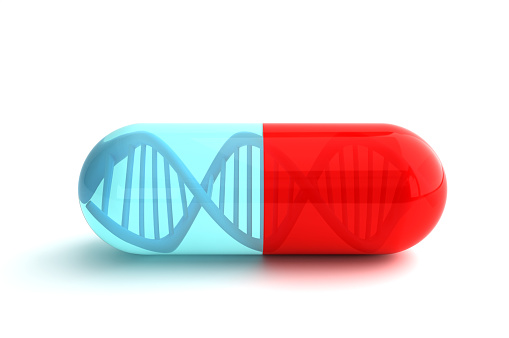
\includegraphics{pilldna}}\\[\baselineskip] % Publisher and logo
}}
\endgroup}

%----------------------------------------------------------------------------------------
%				BLANK DOCUMENT
%----------------------------------------------------------------------------------------

\begin{document}

\pagestyle{empty} % Removes page numbers

\titleGM % This command includes the title page


% ------------- TABLE OF CONTENTS -------------------

\tableofcontents

\newpage

% ----------------  SUMMARY PAGES ----------------------

\section{Patient haplotypes}

\scriptsize

\begin{tabularx}{\textwidth}{sbb}
\textbf{Gene} & \textbf{Phylogenetic method}\footnote{Method using phylogenetic trees to find closest 'relative' to patient alleles. Trees can be seen in Appendix A.} &  \textbf{Set method}\footnote{Method looking for overlap of haplotype non-reference variants and patient non-reference variants. Reference variants are filtered out of both sets prior to comparison. Top 5 hits can be seen in Appendix 2.}  \\
\hline \\ABCB1 & *1 / *2 (PMID: 12893986) & *2 (PMID: 12893986) / *2 (PMID: 12893986) \\ABCC2 & H1 / H2 & H1 / H2 \\ADRB1 & H1 / H1 & H1 / H1 \\ADRB2 & 1 / 1 & 1 / 1 \\APOE & E3 / E2 & E3 / E2 \\CDA & *1A / *1A & *1A / *1B \\CFTR & Reference / Reference & Reference / Reference \\CHRNA5 & haplotype 1 / haplotype 1 & haplotype 1 / haplotype 1 \\COMT & Haplotype low activity / Haplotype high activity & Haplotype low activity / Haplotype high activity \\CYP1A1 & *1 / *1 & *1 / *1 \\CYP1A2 & *1M / *1M & *1M / *1M \\CYP1B1 & *1 / *6 & *1 / *6 \\CYP2A6 & *1A / *2 & *1A / *2 \\CYP2B6 & *1 / *1 & *1 / *1 \\CYP2C19 & *1A / *3B & *1A / *3B \\CYP2C8 & *1A / *1A & *1A / *1A \\CYP2C9 & *1 / *18 & *1 / *3 \\CYP2D6 & *1 / *1E & *1 / *1E \\CYP2E1 & *1A / *1A & *1A / *1A \\CYP3A4 & *1 / *1 & *1 / *1 \\CYP3A43 & *1A / *1A & *1A / *1A \\CYP3A5 & *1A / *1A & *1A / *1A \\CYP4B1 & *1 / *1 & *1 / *1 \\CYP4F2 & *1 / *1 & *1 / *1 \\DDC & \#1 / \#1 & \#1 / \#1 \\DPYD & *1 / *1 & *1 / *1 \\G6PD & B (wildtype) / B (wildtype) & B (wildtype) / B (wildtype) \\HMGCR & H2 / H2 & H7 / H7 \\HNF4A & TATTT / TGCGC & TATTT / TGCGC \\HTR2C & 1--2--1 / 1--2--1 & 1--2--1 / 1--2--1 \\IFNL3 & rs12979860C / rs12979860T & rs12979860C / rs12979860T \\IGFBP3 & 1 / 1 & 1 / 1 \\LDLR & L5 / L1 & L5 / L1 \\NAT1 & *4 / *4 & *4 / *4 \\NAT2 & *6A / *6A & *6A / *6A \\NUDT15 & *1 / *1 & *1 / *1 \\P2RY12 & B / B & B / B \\PIK3CA & H1 / H2 & H1 / H2 \\RXRA & AG / AG & AG / AG \\RYR1 & 571I;3366R;3933Y / 571I;3366R;3933Y & 571I;3366R;3933Y / 571I;3366R;3933Y \\SCN1A & \#1 / \#1 & \#1 / \#2 \\SCNN1B & 1-1 / 1-1 & 1-1 / 1-1 \\SLC22A1 & *1 / *1 & *1 / *1 \\SLCO1B1 & *1A / *20 & *1A / *20 \\STAT3 & TTG / CCG & TTG / CCG \\SULT1A1 & *1 / *2 & *1 / *2 \\SULT1A2 & *1 / *2 & *1 / *2 \\TPMT & *1 / *1 & *1 / *3E \\UGT1A1 & *1 / *60 & *1 / *60 \\UGT1A10 & *1a / *1a & *1a / *1a \\UGT1A3 & *1 / *2a & *1 / *2a \\UGT1A4 & *1a / *1a & *1a / *1a \\UGT1A5 & *1 / *1 & *1 / *1 \\UGT1A6 & *1a / *2e & *1a / *2e \\UGT1A7 & *1a / *3 & *1a / *3 \\UGT1A8 & *1a / *1a & *1a / *1a \\UGT2B15 & *1 / *4 & *1 / *4 \\VEGFA & H1 / H1 & H1 / H1 \\VKORC1 & H1 / H2 & H1 / *2 \\\end{tabularx}

\normalsize

\newpage

\section{Drug annotations}

\scriptsize
\begin{tabularx}{1.3\textwidth}{XXXX}
\textbf{Drug} & \textbf{Level 1-2\footnote{ Level 1A and 1B clinical annotations meet the highest levels of criteria and are manually curated by PharmGKB. Level 1A annotations contain a variant-drug combination in a CPIC or medical society endorsed PGx guideline, or, implemented at a PGRN site, or, in another major health system. Level 1B annotations contain a variant-drug combination where the preponderance of evidence shows an association. The association must be replicated in more than one cohort with significant p-values, and, preferably with a strong effect size. Lower levels (3-4) are less significant and may only be based on a single study or case report, which may be performed in vitro.(PHARMGKB) }} & \textbf{Level 3-4\footnote{ See above }}   \\
\hline \\Ace Inhibitors, Plain &  0 & 2 \\acenocoumarol &  0 & 1 \\acetaminophen &  0 & 30 \\amlodipine &  0 & 5 \\Analgesics &  0 & 1 \\anastrozole &  0 & 0 \\anthracyclines and related substances &  0 & 11 \\antiepileptics &  0 & 1 \\Antiinflammatory agents, non-steroids &  0 & 1 \\antipsychotics &  0 & 4 \\Antivirals for treatment of HIV infections, combinations &  0 & 3 \\atazanavir &  0 & 31 \\atenolol &  0 & 1 \\atorvastatin &  0 & 4 \\benazepril &  0 & 1 \\Beta Blocking Agents &  0 & 2 \\bevacizumab &  0 & 2 \\bupropion &  0 & 2 \\busulfan &  0 & 2 \\capecitabine &  0 & 12 \\carbamazepine &  0 & 14 \\carvedilol &  0 & 9 \\catecholamines &  0 & 1 \\celecoxib &  1 & 0 \\clopidogrel &  0 & 3 \\clozapine &  0 & 2 \\codeine &  0 & 1 \\cotinine &  0 & 2 \\coumarin &  0 & 0 \\cyclophosphamide &  0 & 6 \\cyclosporine &  0 & 7 \\cytarabine &  0 & 3 \\Dabigatran &  0 & 0 \\daunorubicin &  0 & 1 \\deferasirox &  0 & 0 \\diuretics &  0 & 2 \\dobutamine &  0 & 1 \\docetaxel &  0 & 9 \\doxorubicin &  0 & 2 \\Drugs For Treatment Of Tuberculosis &  0 & 7 \\efavirenz &  0 & 0 \\enalapril &  0 & 2 \\erlotinib &  0 & 1 \\escitalopram &  0 & 1 \\ethambutol &  0 & 1 \\ethanol &  0 & 2 \\etoposide &  0 & 1 \\fexofenadine &  0 & 1 \\fluorouracil &  0 & 0 \\fluvastatin &  0 & 3 \\gefitinib &  0 & 1 \\gemcitabine &  0 & 1 \\haloperidol &  0 & 1 \\hmg coa reductase inhibitors &  0 & 2 \\iloperidone &  0 & 1 \\imatinib &  0 & 7 \\irbesartan &  0 & 2 \\irinotecan &  0 & 29 \\isoniazid &  0 & 1 \\ivacaftor &  1 & 0 \\lamivudine &  0 & 1 \\lamotrigine &  7 & 0 \\lorazepam &  1 & 0 \\losartan &  0 & 2 \\mercaptopurine &  0 & 0 \\methadone &  0 & 3 \\methotrexate &  0 & 4 \\metoprolol &  0 & 1 \\midazolam &  0 & 0 \\morphine &  0 & 1 \\nevirapine &  0 & 6 \\nicotine &  0 & 0 \\nifedipine &  0 & 0 \\ondansetron &  0 & 3 \\opioids &  0 & 2 \\Opium alkaloids and derivatives &  0 & 2 \\paclitaxel &  0 & 0 \\peginterferon alfa-2a &  0 & 3 \\peginterferon alfa-2b &  0 & 3 \\phenprocoumon &  2 & 0 \\phenytoin &  1 & 0 \\Platinum compounds &  0 & 2 \\pravastatin &  0 & 1 \\propofol &  0 & 0 \\Pyrimidine analogues &  0 & 1 \\quetiapine &  0 & 2 \\raloxifene &  0 & 1 \\ranibizumab &  0 & 1 \\repaglinide &  0 & 2 \\rifampin &  0 & 3 \\risperidone &  0 & 3 \\ritonavir &  0 & 32 \\rosiglitazone &  0 & 1 \\sildenafil &  0 & 1 \\simvastatin &  0 & 0 \\sorafenib &  0 & 7 \\sulfonamides, urea derivatives &  0 & 1 \\sunitinib &  0 & 5 \\tacrolimus &  0 & 0 \\tamoxifen &  0 & 0 \\tegafur &  0 & 0 \\thalidomide &  0 & 2 \\ticagrelor &  0 & 2 \\tolbutamide &  0 & 0 \\tramadol &  0 & 3 \\valproic acid &  0 & 5 \\venlafaxine &  0 & 0 \\verapamil &  0 & 2 \\vitamin e &  0 & 0 \\warfarin &  0 & 16 \\zidovudine &  0 & 1 \\\end{tabularx}

\normalsize

\newpage

% ----------------  Guidelines ----------------------

\section{Haplotype Guidelines}

      

    

      Current drug: NULL

      \subsection{ acenocoumarol }
        \subsubsection{ CYP2C9 }
      \textit{ cytochrome P450, family 2, subfamily C, polypeptide 9 }
      \begin{center}
      Patient haplotype
      \textbf{ *1/*18 } | \textbf{ *1/*3\footnote{For alternate close matches see Appendix II.} } \newline\newline
      \scriptsize
      \begin{tabularx}{\textwidth}{ssbb}
      \textbf{ Check INR more frequently after initiating or discontinuing NSAIDs in individuals taking acenocoumarol with at least one CYP2C9 *2 or *3 allele. }
      & Genotype & Therapeutic Dose Recommendation & Level of Evidence & Clinical Relevance &
\\& --- & --- & --- & --- &
\\& CYP2C9 *1/*2 & Check INR more frequently after initiating or discontinuing NSAIDs & Published controlled studies of good quality* relating to phenotyped and/or genotyped patients or healthy volunteers, and having relevant pharmacokinetic or clinical endpoints. & Minor clinical effect (S): QTc prolongation (&lt;450 ms females, &lt;470 ms males); INR increase &lt;4.5. Kinetic effect (S) &
\\& CYP2C9 *2/*2 & Check INR more frequently after initiating or discontinuing NSAIDs & Published controlled studies of good quality* relating to phenotyped and/or genotyped patients or healthy volunteers, and having relevant pharmacokinetic or clinical endpoints. & Minor clinical effect (S): QTc prolongation (&lt;450 ms females, &lt;470 ms males); INR increase &lt;4.5. Kinetic effect (S) &
\\& CYP2C9 *1/*3 & Check INR more frequently after initiating or discontinuing NSAIDs & Published controlled studies of good quality* relating to phenotyped and/or genotyped patients or healthy volunteers, and having relevant pharmacokinetic or clinical endpoints. & Clinical effect (S): short-lived discomfort (&lt; 48 hr) without permanent injury: e.g. reduced decrease in resting heart rate; reduction in exercise tachycardia; decreased pain relief from oxycodone; ADE resulting from increased bioavailability of atomoxetine (decreased appetite, insomnia, sleep disturbance etc); neutropenia &gt; 1.5x10^9^/l; leucopenia &gt; 3.0x10^9^/l; thrombocytopenia  &gt; 75x10^9^/l; moderate diarrhea not affecting daily activities; reduced glucose increase following oral glucose tolerance test. &
\\& CYP2C9 *2/*3 & Check INR more frequently after initiating or discontinuing NSAIDs & Published controlled studies of good quality* relating to phenotyped and/or genotyped patients or healthy volunteers, and having relevant pharmacokinetic or clinical endpoints. & Minor clinical effect (S): QTc prolongation (&lt;450 ms females, &lt;470 ms males); INR increase &lt;4.5. Kinetic effect (S) &
\\& CYP2C9 *3/*3 & Check INR more frequently during dose titration and after initiating or discontinuing NSAIDs & Published controlled studies of good quality* relating to phenotyped and/or genotyped patients or healthy volunteers, and having relevant pharmacokinetic or clinical endpoints. & Minor clinical effect (S): QTc prolongation (&lt;450 ms females, &lt;470 ms males); INR increase &lt;4.5. Kinetic effect (S) &
\\
      \end{tabularx}
      \end{center}

      

    

      Current drug: NULL

      \subsection{ acenocoumarol }
        \subsubsection{ VKORC1 }
      \textit{ vitamin K epoxide reductase complex, subunit 1 }
      \begin{center}
      Patient haplotype
      \textbf{ H1/H2 } | \textbf{ H1/*2\footnote{For alternate close matches see Appendix II.} } \newline\newline
      \scriptsize
      \begin{tabularx}{\textwidth}{ssbb}
      \textbf{ While VKORC1 genotype has been found to contribute to acenocoumarol dose variability, there are no dosing recommendations at this time. Check INR more frequently in patients with the AA genotype at [variant:rs9934438]. }
      & Genotype & Therapeutic Dose Recommendation & Level of Evidence & Clinical Relevance &
\\& --- & --- & --- & --- &
\\& VKORC1 [variant:rs9934438] AG & None & Published controlled studies of good quality* relating to phenotyped and/or genotyped patients or healthy volunteers, and having relevant pharmacokinetic or clinical endpoints. & Minor clinical effect (S): QTc prolongation (&lt;450 ms , &lt;470 ms ); INR increase &lt; 4.5; Kinetic effect (S). & 
\\& VKORC1 [variant:rs9934438] AA & Check INR more frequently. & Published controlled studies of good quality* relating to phenotyped and/or genotyped patients or healthy volunteers, and having relevant pharmacokinetic or clinical endpoints. & Minor clinical effect (S): QTc prolongation (&lt;450 ms , &lt;470 ms ); INR increase &lt; 4.5; Kinetic effect (S). &
\\
      \end{tabularx}
      \end{center}

      

    

      Current drug: NULL

      \subsection{ atazanavir }
        \subsubsection{ UGT1A1 }
      \textit{ UDP glucuronosyltransferase 1 family, polypeptide A1 }
      \begin{center}
      Patient haplotype
      \textbf{ *1/*60 } | \textbf{ *1/*60\footnote{For alternate close matches see Appendix II.} } \newline\newline
      \scriptsize
      \begin{tabularx}{\textwidth}{ssbb}
      \textbf{ The CPIC dosing guideline recommends considering advising individuals who carry two decreased function -UGT1A1- alleles about a substantial likelihood of developing jaundice, which may cause non-adherence. The dosing guideline recommends that alternative agents be considered if the risk of non-adherence due to jaundice is high. The risk of discontinuation is low and very low for individuals carrying one, or no decreased function -UGT1A1- alleles, respectively. }
      & Likely phenotype & Genotypes & Examples of diplotypes & Implications for phenotypic measures   & Recommendations for atazanavir therapy & Classification of recommendation for atazanavir therapy &
\\& --- & --- & --- & --- & --- & --- &
\\&Extensive Metabolizer & An individual carrying 2 reference ^b^ function and/or increased function alleles; or individuals of genotype CC at [variant:rs887829] & *1/*1; *1/*36; *36/*36; [variant:rs887829] CC& Reference ^c^ UGT1A1 activity; very low likelihood of bilirubin-related discontinuation of atazanavir.  &  There is no need to avoid prescribing of atazanavir based on -UGT1A1- genetic test result.  &  Strong &
\\&Intermediate Metabolizer  & An individual carrying one reference ^b^ function (*1) ^c^ or increased function allele (*36) plus one decreased function allele (*6, *28, *37). Alternatively identified by heterozygosity for [variant:rs887829] C/T. & *1/*28; *1/*37; *36/*28; *36/*37; [variant:rs887829] C/T, *1/*6 & Somewhat decreased UGT1A1 activity; low likelihood of bilirubin-related discontinuation of atazanavir. & There is no need to avoid prescribing of atazanavir based on -UGT1A1- genetic test result. Inform the patient that some patients stop atazanavir because of jaundice (yellow eyes and skin), but that this patient’s genotype makes this unlikely &  Strong &
\\&Poor Metabolizer  & An individual carrying two decreased function alleles (*6, *28, *37). Alternatively identified by homozygosity for [variant:rs887829] T/T (*80/*80) & *28/*28; *28/*37; *37/*37; [variant:rs887829] T/T (*80/*80), *6/*6 ^a^ & Markedly decreased UGT1A1 activity; high likelihood of bilirubin-related discontinuation of atazanavir. & Consider an alternative agent particularly where jaundice would be of concern to the patient. &  Strong &
\\
      \end{tabularx}
      \end{center}

      

    

      Current drug: NULL

      \subsection{ capecitabine }
        \subsubsection{ DPYD }
      \textit{ dihydropyrimidine dehydrogenase }
      \begin{center}
      Patient haplotype
      \textbf{ *1/*1 } | \textbf{ *1/*1\footnote{For alternate close matches see Appendix II.} } \newline\newline
      \scriptsize
      \begin{tabularx}{\textwidth}{ssbb}
      \textbf{ The CPIC Dosing Guidelines for fluoropyrimidines (i.e. 5-fluorouracil, capecitabine or tegafur) recommends an alternative drug for patients who are homozygous for DPYD non-functional variants - *2A ([variant:rs3918290]), *13 ([variant:rs55886062]), and [variant:rs67376798] A (on the positive chromosomal strand) - as these patients are typically DPD deficient.  Consider a 50\% reduction in starting dose for heterozygous patients (intermediate activity). }
      & Phenotype (genotype) & Examples of diplotypes & Implications for phenotypic measures & Dosing recommendations & Classification of recommendations ^a^ &
\\& --- & --- & --- & --- & --- &
\\& Homozygous wild-type or normal, high DPD activity (two or more functional *1 alleles) & *1/*1 & Normal DPD activity and &\#34;normal&\#34; risk for fluoropyrimidine toxicity & Use label-recommended dosage and administration & Moderate &
\\& Heterozygous or intermediate activity (~3-5\% of patients), may have partial DPD deficiency, at risk for toxicity with drug exposure (one functional allele *1, plus one nonfunctional allele - *2A, *13 or rs67376798A ^c^) & *1/*2A; *1/*13; *1/ rs67376798A ^c^) & Decreased DPD activity (leukocyte DPD activity at 30\% to 70\% that of the normal population) and increased risk for severe or even fatal drug toxicity when treated with fluoropyrimidine drugs & Start with at least a 50\% reduction in starting dose followed by titration of dose based on toxicity ^b^ or pharmacokinetic test (if available) & Moderate &
\\& Homozygous variant, DPD deficiency (~0.2\% of patients), at risk for toxicity with drug exposure (2 nonfunctional alleles - *2A, *13 or rs67376798A ^c^) & *2A/*2A; *13/*13; rs67376798A ^c^ / rs67376798A ^c^ & Complete DPD deficiency and increased risk for severe or even fatal drug toxicity when treated with fluoropyrimidine drugs & Select alternate drug & Strong &
\\
      \end{tabularx}
      \end{center}

      

    

      Current drug: NULL

      \subsection{ capecitabine }
        \subsubsection{ DPYD }
      \textit{ dihydropyrimidine dehydrogenase }
      \begin{center}
      Patient haplotype
      \textbf{ *1/*1 } | \textbf{ *1/*1\footnote{For alternate close matches see Appendix II.} } \newline\newline
      \scriptsize
      \begin{tabularx}{\textwidth}{ssbb}
      \textbf{ The CPIC Dosing Guidelines for fluoropyrimidines (i.e. 5-fluorouracil, capecitabine or tegafur) recommends an alternative drug for patients who are homozygous for DPYD non-functional variants - *2A ([variant:rs3918290]), *13 ([variant:rs55886062]), and [variant:rs67376798] A (on the positive chromosomal strand) - as these patients are typically DPD deficient.  Consider a 50\% reduction in starting dose for heterozygous patients (intermediate activity). }
      & Phenotype (genotype) & Examples of diplotypes & Implications for phenotypic measures & Dosing recommendations & Classification of recommendations ^a^ &
\\& --- & --- & --- & --- & --- &
\\& Homozygous wild-type or normal, high DPD activity (two or more functional *1 alleles) & *1/*1 & Normal DPD activity and &\#34;normal&\#34; risk for fluoropyrimidine toxicity & Use label-recommended dosage and administration & Moderate &
\\& Heterozygous or intermediate activity (~3-5\% of patients), may have partial DPD deficiency, at risk for toxicity with drug exposure (one functional allele *1, plus one nonfunctional allele - *2A, *13 or rs67376798A ^c^) & *1/*2A; *1/*13; *1/ rs67376798A ^c^) & Decreased DPD activity (leukocyte DPD activity at 30\% to 70\% that of the normal population) and increased risk for severe or even fatal drug toxicity when treated with fluoropyrimidine drugs & Start with at least a 50\% reduction in starting dose followed by titration of dose based on toxicity ^b^ or pharmacokinetic test (if available) & Moderate &
\\& Homozygous variant, DPD deficiency (~0.2\% of patients), at risk for toxicity with drug exposure (2 nonfunctional alleles - *2A, *13 or rs67376798A ^c^) & *2A/*2A; *13/*13; rs67376798A ^c^ / rs67376798A ^c^ & Complete DPD deficiency and increased risk for severe or even fatal drug toxicity when treated with fluoropyrimidine drugs & Select alternate drug & Strong &
\\
      \end{tabularx}
      \end{center}

      

    

      Current drug: NULL

      \subsection{ fluorouracil }
        \subsubsection{ DPYD }
      \textit{ dihydropyrimidine dehydrogenase }
      \begin{center}
      Patient haplotype
      \textbf{ *1/*1 } | \textbf{ *1/*1\footnote{For alternate close matches see Appendix II.} } \newline\newline
      \scriptsize
      \begin{tabularx}{\textwidth}{ssbb}
      \textbf{ The CPIC Dosing Guidelines for fluoropyrimidines (i.e. 5-fluorouracil, capecitabine or tegafur) recommends an alternative drug for patients who are homozygous for DPYD non-functional variants - *2A ([variant:rs3918290]), *13 ([variant:rs55886062]), and [variant:rs67376798] A (on the positive chromosomal strand) - as these patients are typically DPD deficient.  Consider a 50\% reduction in starting dose for heterozygous patients (intermediate activity). }
      & Phenotype (genotype) & Examples of diplotypes & Implications for phenotypic measures & Dosing recommendations & Classification of recommendations^a^ &
\\& --- & --- & --- & --- & --- &
\\& Homozygous wild-type or normal, high DPD activity (two or more functional *1 alleles) & *1/*1 & Normal DPD activity and &\#34;normal&\#34; risk for fluoropyrimidine toxicity & Use label-recommended dosage and administration & Moderate &
\\& Heterozygous or intermediate activity (~3-5\% of patients), may have partial DPD deficiency, at risk for toxicity with drug exposure (one functional allele *1, plus one nonfunctional allele - *2A, *13 or rs67376798A^c^) & *1/*2A; *1/*13; *1/ rs67376798A^c^) & Decreased DPD activity (leukocyte DPD activity at 30\% to 70\% that of the normal population) and increased risk for severe or even fatal drug toxicity when treated with fluoropyrimidine drugs & Start with at least a 50\% reduction in starting dose followed by titration of dose based on toxicity ^b^ or pharmacokinetic test (if available) & Moderate &
\\& Homozygous variant, DPD deficiency (~0.2\% of patients), at risk for toxicity with drug exposure (2 nonfunctional alleles - *2A, *13 or rs67376798A ^c^) & *2A/*2A; *13/*13; rs67376798A^c^ / rs67376798A^c^ & Complete DPD deficiency and increased risk for severe or even fatal drug toxicity when treated with fluoropyrimidine drugs & Select alternate drug & Strong &
\\
      \end{tabularx}
      \end{center}

      

    

      Current drug: NULL

      \subsection{ fluorouracil }
        \subsubsection{ DPYD }
      \textit{ dihydropyrimidine dehydrogenase }
      \begin{center}
      Patient haplotype
      \textbf{ *1/*1 } | \textbf{ *1/*1\footnote{For alternate close matches see Appendix II.} } \newline\newline
      \scriptsize
      \begin{tabularx}{\textwidth}{ssbb}
      \textbf{ The CPIC Dosing Guidelines for fluoropyrimidines (i.e. 5-fluorouracil, capecitabine or tegafur) recommends an alternative drug for patients who are homozygous for DPYD non-functional variants - *2A ([variant:rs3918290]), *13 ([variant:rs55886062]), and [variant:rs67376798] A (on the positive chromosomal strand) - as these patients are typically DPD deficient.  Consider a 50\% reduction in starting dose for heterozygous patients (intermediate activity). }
      & Phenotype (genotype) & Examples of diplotypes & Implications for phenotypic measures & Dosing recommendations & Classification of recommendations^a^ &
\\& --- & --- & --- & --- & --- &
\\& Homozygous wild-type or normal, high DPD activity (two or more functional *1 alleles) & *1/*1 & Normal DPD activity and &\#34;normal&\#34; risk for fluoropyrimidine toxicity & Use label-recommended dosage and administration & Moderate &
\\& Heterozygous or intermediate activity (~3-5\% of patients), may have partial DPD deficiency, at risk for toxicity with drug exposure (one functional allele *1, plus one nonfunctional allele - *2A, *13 or rs67376798A^c^) & *1/*2A; *1/*13; *1/ rs67376798A^c^) & Decreased DPD activity (leukocyte DPD activity at 30\% to 70\% that of the normal population) and increased risk for severe or even fatal drug toxicity when treated with fluoropyrimidine drugs & Start with at least a 50\% reduction in starting dose followed by titration of dose based on toxicity ^b^ or pharmacokinetic test (if available) & Moderate &
\\& Homozygous variant, DPD deficiency (~0.2\% of patients), at risk for toxicity with drug exposure (2 nonfunctional alleles - *2A, *13 or rs67376798A ^c^) & *2A/*2A; *13/*13; rs67376798A^c^ / rs67376798A^c^ & Complete DPD deficiency and increased risk for severe or even fatal drug toxicity when treated with fluoropyrimidine drugs & Select alternate drug & Strong &
\\
      \end{tabularx}
      \end{center}

      

    

      Current drug: NULL

      \subsection{ irinotecan }
        \subsubsection{ UGT1A1 }
      \textit{ UDP glucuronosyltransferase 1 family, polypeptide A1 }
      \begin{center}
      Patient haplotype
      \textbf{ *1/*60 } | \textbf{ *1/*60\footnote{For alternate close matches see Appendix II.} } \newline\newline
      \scriptsize
      \begin{tabularx}{\textwidth}{ssbb}
      \textbf{ A French joint working group comprising the National Pharmacogenetics Network (RNPGx) and the Group of Clinical Onco-pharmacology (GPCO-Unicancer) has published guidelines for the use of -UGT1A1*28- genotype when prescribing irinotecan. They recommend that the dose of irinotecan be reduced in patients with the -UGT1A1*28/*28- genotype, and that high-dose irinotecan (&gt;=240 mg/m2) only be prescribed to patients with the -UGT1A1*1/*1- genotype. }
      -^Reprinted with permission from Etienne-Grimaldi et al. UGT1A1 genotype and irinotecan therapy: general review and implementation in routine practice. Fundamental &amp; Clinical Pharmacology (2015)^-\\
      \end{tabularx}
      \end{center}

      

    

      Current drug: NULL

      \subsection{ irinotecan }
        \subsubsection{ UGT1A1 }
      \textit{ UDP glucuronosyltransferase 1 family, polypeptide A1 }
      \begin{center}
      Patient haplotype
      \textbf{ *1/*60 } | \textbf{ *1/*60\footnote{For alternate close matches see Appendix II.} } \newline\newline
      \scriptsize
      \begin{tabularx}{\textwidth}{ssbb}
      \textbf{ A French joint working group comprising the National Pharmacogenetics Network (RNPGx) and the Group of Clinical Onco-pharmacology (GPCO-Unicancer) has published guidelines for the use of -UGT1A1*28- genotype when prescribing irinotecan. They recommend that the dose of irinotecan be reduced in patients with the -UGT1A1*28/*28- genotype, and that high-dose irinotecan (&gt;=240 mg/m2) only be prescribed to patients with the -UGT1A1*1/*1- genotype. }
      -^Reprinted with permission from Etienne-Grimaldi et al. UGT1A1 genotype and irinotecan therapy: general review and implementation in routine practice. Fundamental &amp; Clinical Pharmacology (2015)^-\\
      \end{tabularx}
      \end{center}

      

    

      Current drug: NULL

      \subsection{ ivacaftor }
        \subsubsection{ CFTR }
      \textit{ cystic fibrosis transmembrane conductance regulator (ATP-binding cassette sub-family C, member 7) }
      \begin{center}
      Patient haplotype
      \textbf{ Reference/Reference } | \textbf{ Reference/Reference\footnote{For alternate close matches see Appendix II.} } \newline\newline
      \scriptsize
      \begin{tabularx}{\textwidth}{ssbb}
      \textbf{ Ivacaftor treatment is recommended only in cystic fibrosis (CF) patients that are either homozygous or heterozygous for certain -CFTR- variants.  See full guideline for disclaimers, further details and supporting evidence. }
      & CFTR Genotype & Examples of diplotypes & Implications for ivacaftor effects & Recommendations for ivacaftor therapy & Classification of recommendation for ivacaftor therapy^c^&
\\& --- & --- & --- & --- & --- &
\\& Homozygous or Heterozygous G551D-CFTR, [variant:rs75527207] genotype AA or AG & G551D/ F508del, G551D/ G551D & Significant improvement in lung function, weight, risk of pulmonary exacerbation, patient reported outcomes, and reduction in sweat chloride concentrations through enhanced CFTR channel activity (increase probability of open channel). & Use ivacaftor according to the product label & Strong & 
\\& Homozygous for F508del-CFTR, [variant:rs113993960] or [variant:rs199826652] genotype del/del & F508del/F508del& No significant reduction in sweat chloride concentrations; no changes in other clinical measurements including spirometric measurements, pulmonary exacerbations, or body weight^b^. Unlikely to respond to treatment. & Ivacaftor is not recommended^a^ & Moderate^b^ & 
\\&Homozygous or heterozygous for one of the following -CFTR- variants: G1244E ([variant:rs267606723] genotype AA or AG), G1349D ([variant:rs193922525] genotype AA or AG), G178R ([variant:rs80282562] genotype AA or AG), G551S ([variant:rs121909013] genotype AA or AG), S1251N ([variant:rs74503330] genotype AA or AG), S1255P ([variant:rs121909041] genotype CC or CT), S549N ([variant:rs121908755] genotype AA or AG), S549R ([variant:rs121909005] genotype GG or GT, [variant:rs121908757] genotype AC or CC), R117H ([variant:rs78655421] genotype AA or AG)^d^  & F508del/S549N & Significantly enhanced channel open probability -in vitro- [PMID: 22293084]. -In vitro- assays with CFBEo- cells expressing S549N-CFTR showed ivacaftor potentiated chloride channel function [PMID: 23027855], and a case study showed improved lung function after ivacaftor treatment in a 12-year-old girl with CF with a copy of the S549N variant [PMID: 24081349]. Improvement in sweat chloride and CFQ-R respiratory domain scores in patients with the R117H variant [PMID: 26070913] & Use ivacaftor according to the product label & Moderate &
\\
      \end{tabularx}
      \end{center}

      

    

      Current drug: NULL

      \subsection{ mercaptopurine }
        \subsubsection{ TPMT }
      \textit{ thiopurine S-methyltransferase }
      \begin{center}
      Patient haplotype
      \textbf{ *1/*1 } | \textbf{ *1/*3E\footnote{For alternate close matches see Appendix II.} } \newline\newline
      \scriptsize
      \begin{tabularx}{\textwidth}{ssbb}
      \textbf{ Select an alternative drug or reduce the initial dose for intermediate or poor metabolizers. }
      & Phenotype (Genotype) & Therapeutic Dose Recommendation & Level of Evidence & Clinical Relevance &
\\& --- & --- & --- & --- &
\\& IM (one inactive allele: *2, *3, *4-*18) & Select alternative drug or reduce dose by 50\%. Increase dose in response of hematologic monitoring and efficacy. & Published controlled studies of good quality* relating to phenotyped and/or genotyped patients or healthy volunteers, and having relevant pharmacokinetic or clinical endpoints. & Clinical effect (S): Failure of lifesaving therapy e.g. anticipated myelosuppression; prevention of breast cancer relapse; arrhythmia; neutropenia &lt; 0.5x10^9^/l; leucopenia &lt; 1.0x10^9^/l; thrombocytopenia &lt; 25x10^9^/l; life-threatening complications from diarrhea. &
\\& PM (two inactive alleles: *2, *3, *4-*18) & Select alternative drug or reduce dose by 90\%. Increase dose in response of hematologic monitoring and efficacy. & Published controlled studies of good quality* relating to phenotyped and/or genotyped patients or healthy volunteers, and having relevant pharmacokinetic or clinical endpoints. & Clinical effect (S): death; arrhythmia; unanticipated myelosuppression. &
\\
      \end{tabularx}
      \end{center}

      

    

      Current drug: NULL

      \subsection{ mercaptopurine }
        \subsubsection{ TPMT }
      \textit{ thiopurine S-methyltransferase }
      \begin{center}
      Patient haplotype
      \textbf{ *1/*1 } | \textbf{ *1/*3E\footnote{For alternate close matches see Appendix II.} } \newline\newline
      \scriptsize
      \begin{tabularx}{\textwidth}{ssbb}
      \textbf{ Select an alternative drug or reduce the initial dose for intermediate or poor metabolizers. }
      & Phenotype (Genotype) & Therapeutic Dose Recommendation & Level of Evidence & Clinical Relevance &
\\& --- & --- & --- & --- &
\\& IM (one inactive allele: *2, *3, *4-*18) & Select alternative drug or reduce dose by 50\%. Increase dose in response of hematologic monitoring and efficacy. & Published controlled studies of good quality* relating to phenotyped and/or genotyped patients or healthy volunteers, and having relevant pharmacokinetic or clinical endpoints. & Clinical effect (S): Failure of lifesaving therapy e.g. anticipated myelosuppression; prevention of breast cancer relapse; arrhythmia; neutropenia &lt; 0.5x10^9^/l; leucopenia &lt; 1.0x10^9^/l; thrombocytopenia &lt; 25x10^9^/l; life-threatening complications from diarrhea. &
\\& PM (two inactive alleles: *2, *3, *4-*18) & Select alternative drug or reduce dose by 90\%. Increase dose in response of hematologic monitoring and efficacy. & Published controlled studies of good quality* relating to phenotyped and/or genotyped patients or healthy volunteers, and having relevant pharmacokinetic or clinical endpoints. & Clinical effect (S): death; arrhythmia; unanticipated myelosuppression. &
\\
      \end{tabularx}
      \end{center}

      

    

      Current drug: NULL

      \subsection{ peginterferon alfa-2a }
        \subsubsection{ IFNL3 }
      \textit{ interferon, lambda 3 }
      \begin{center}
      Patient haplotype
      \textbf{ rs12979860C/rs12979860T } | \textbf{ rs12979860C/rs12979860T\footnote{For alternate close matches see Appendix II.} } \newline\newline
      \scriptsize
      \begin{tabularx}{\textwidth}{ssbb}
      \textbf{ IFNL3 (IL28B) variation ([variant:rs12979860]) is the strongest baseline predictor of response to PEG-interferon-alpha-containing regimens in HCV genotype 1 patients.  Patients with the favorable response genotype ([variant:rs12979860] CC) have increased likelihood of response (higher SVR rate) to PEG-interferon-alpha-containing regimens as compared to patients with unfavorable response genotype ([variant:rs12979860] CT or TT). Consider implications before initiating PEG-IFN alpha and RBV containing regimens. }
      & Genotype at [variant:rs12979860] & Phenotype & Implications for PEG-IFN alpha and RBV ^a^ & Implications for protease inhibitor combinations with PEG-IFN alpha and RBV therapy & Classification of recommendations ^b^ &
\\& --- & --- & --- & --- & --- &
\\& CC & Favorable response genotype & Approximately 70\% chance for SVR ^c^ after 48 weeks of treatment. Consider implications before initiating PEG-IFN alpha and RBV containing regimens. & Approximately 90\% chance for SVR after 24-48 weeks of treatment. Approximately 80-90\% of patients are eligible for shortened therapy (24-28 weeks vs. 48 weeks)^d^. Weighs in favor of using PEG-IFN alpha and RBV containing regimens.& Strong &
\\& CT or TT & Unfavorable response genotype & Approximately 30\% chance for SVR ^c^ after 48 weeks of treatment. Consider implications before initiating PEG-IFN alpha and RBV containing regimens. & Approximately 60\% chance for SVR after 24-48 weeks of treatment. Approximately 50\% of patients are eligible for shortened therapy (24-28 weeks)^d^. Consider implications before initiating PEG-IFN and RBV containing regimens.& Strong &
\\
      \end{tabularx}
      \end{center}

      

    

      Current drug: NULL

      \subsection{ peginterferon alfa-2b }
        \subsubsection{ IFNL3 }
      \textit{ interferon, lambda 3 }
      \begin{center}
      Patient haplotype
      \textbf{ rs12979860C/rs12979860T } | \textbf{ rs12979860C/rs12979860T\footnote{For alternate close matches see Appendix II.} } \newline\newline
      \scriptsize
      \begin{tabularx}{\textwidth}{ssbb}
      \textbf{ IFNL3 (IL28B) variation ([variant:rs12979860]) is the strongest baseline predictor of response to PEG-interferon-alpha-containing regimens in HCV genotype 1 patients.  Patients with the favorable response genotype ([variant:rs12979860] CC) have increased likelihood of response (higher SVR rate) to PEG-interferon-alpha-containing regimens as compared to patients with unfavorable response genotype ([variant:rs12979860] CT or TT). Consider implications before initiating PEG-IFN alpha and RBV containing regimens. }
      & Genotype at [variant:rs12979860] & Phenotype & Implications for PEG-IFN alpha and RBV ^a^ & Implications for protease inhibitor combinations with PEG-IFN alpha and RBV therapy & Classification of recommendations ^b^ &
\\& --- & --- & --- & --- & --- &
\\& CC & Favorable response genotype & Approximately 70\% chance for SVR ^c^ after 48 weeks of treatment. Consider implications before initiating PEG-IFN alpha and RBV containing regimens. & Approximately 90\% chance for SVR after 24-48 weeks of treatment. Approximately 80-90\% of patients are eligible for shortened therapy (24-28 weeks vs. 48 weeks)^d^. Weighs in favor of using PEG-IFN alpha and RBV containing regimens.& Strong &
\\& CT or TT & Unfavorable response genotype & Approximately 30\% chance for SVR ^c^ after 48 weeks of treatment. Consider implications before initiating PEG-IFN alpha and RBV containing regimens. & Approximately 60\% chance for SVR after 24-48 weeks of treatment. Approximately 50\% of patients are eligible for shortened therapy (24-28 weeks)^d^. Consider implications before initiating PEG-IFN and RBV containing regimens.& Strong &
\\
      \end{tabularx}
      \end{center}

      

    

      Current drug: NULL

      \subsection{ phenprocoumon }
        \subsubsection{ VKORC1 }
      \textit{ vitamin K epoxide reductase complex, subunit 1 }
      \begin{center}
      Patient haplotype
      \textbf{ H1/H2 } | \textbf{ H1/*2\footnote{For alternate close matches see Appendix II.} } \newline\newline
      \scriptsize
      \begin{tabularx}{\textwidth}{ssbb}
      \textbf{ For patients treated with phenprocoumon, consider checking INR more frequently in patients with the AA genotype at VKORC1 [variant:rs9934438]. }
      & Genotype & Therapeutic Dose Recommendation & Level of Evidence & Clinical Relevance &
\\& --- & --- & --- & --- &
\\& VKORC1 [variant:rs9934438] AG & None & Published controlled studies of good quality* relating to phenotyped and/or genotyped patients or healthy volunteers, and having relevant pharmacokinetic or clinical endpoints. & Minor clinical effect (S): QTc prolongation (&lt;450 ms , &lt;470 ms); INR increase &lt; 4.5 Kinetic effect (S). &
\\& VKORC1 [variant:rs9934438] AA & Check INR more frequently. & Published controlled studies of good quality* relating to phenotyped and/or genotyped patients or healthy volunteers, and having relevant pharmacokinetic or clinical endpoints. & Minor clinical effect (S): QTc prolongation (&lt;450 ms , &lt;470 ms); INR increase &lt; 4.5 Kinetic effect (S). &
\\
      \end{tabularx}
      \end{center}

      

    

      Current drug: NULL

      \subsection{ tacrolimus }
        \subsubsection{ CYP3A5 }
      \textit{ cytochrome P450, family 3, subfamily A, polypeptide 5 }
      \begin{center}
      Patient haplotype
      \textbf{ *1A/*1A } | \textbf{ *1A/*1A\footnote{For alternate close matches see Appendix II.} } \newline\newline
      \scriptsize
      \begin{tabularx}{\textwidth}{ssbb}
      \textbf{ The CPIC dosing guideline for tacrolimus recommends increasing the starting dose by 1.5 to 2 times the recommended starting dose in patients who are CYP3A5 intermediate or extensive metabolizers, though total starting dose should not exceed 0.3 mg/kg/day. Therapeutic drug monitoring should also be used to guide dose adjustments. }
      & Likely phenotype ^a^ & Genotypes & Examples of diplotypes ^b^ & Implications for tacrolimus pharmacologic measures & Therapeutic Recommendations ^c^ & Classification of recommendations ^e^ &
\\& --- & --- & --- & --- & --- & --- &
\\& Extensive metabolizer (CYP3A5 expresser) & An individual carrying two functional alleles & *1/*1 & Lower dose-adjusted trough concentrations of tacrolimus and decreased chance of achieving target tacrolimus concentrations & Increase starting dose 1.5 to 2 times recommended starting dose ^d^. Total starting dose should not exceed 0.3mg/kg/day. Use therapeutic drug monitoring to guide dose adjustments & Strong &
\\& Intermediate metabolizer (CYP3A5 expresser) & An individual carrying one functional allele and one non-functional allele & *1/*3, *1/*6, *1/*7& Lower dose-adjusted trough concentrations of tacrolimus and decreased chance of achieving target tacrolimus concentrations & Increase starting dose 1.5 to 2 times recommended starting dose ^d^. Total starting dose should not exceed 0.3mg/kg/day. Use therapeutic drug monitoring to guide dose adjustments & Strong &
\\& Poor metabolizer (CYP3A5 non-expresser) & An individual carrying two non-functional alleles & *3/*3, *6/*6, *7/*7, *3/*6, *3/*7, *6/*7& Higher (“normal”) dose-adjusted trough concentrations of tacrolimus and increased chance of achieving target tacrolimus concentrations & Initiate therapy with standard recommended dose. Use therapeutic drug monitoring to guide dose adjustments & Strong &
\\
      \end{tabularx}
      \end{center}

      

    

      Current drug: NULL

      \subsection{ tacrolimus }
        \subsubsection{ CYP3A5 }
      \textit{ cytochrome P450, family 3, subfamily A, polypeptide 5 }
      \begin{center}
      Patient haplotype
      \textbf{ *1A/*1A } | \textbf{ *1A/*1A\footnote{For alternate close matches see Appendix II.} } \newline\newline
      \scriptsize
      \begin{tabularx}{\textwidth}{ssbb}
      \textbf{ The CPIC dosing guideline for tacrolimus recommends increasing the starting dose by 1.5 to 2 times the recommended starting dose in patients who are CYP3A5 intermediate or extensive metabolizers, though total starting dose should not exceed 0.3 mg/kg/day. Therapeutic drug monitoring should also be used to guide dose adjustments. }
      & Likely phenotype ^a^ & Genotypes & Examples of diplotypes ^b^ & Implications for tacrolimus pharmacologic measures & Therapeutic Recommendations ^c^ & Classification of recommendations ^e^ &
\\& --- & --- & --- & --- & --- & --- &
\\& Extensive metabolizer (CYP3A5 expresser) & An individual carrying two functional alleles & *1/*1 & Lower dose-adjusted trough concentrations of tacrolimus and decreased chance of achieving target tacrolimus concentrations & Increase starting dose 1.5 to 2 times recommended starting dose ^d^. Total starting dose should not exceed 0.3mg/kg/day. Use therapeutic drug monitoring to guide dose adjustments & Strong &
\\& Intermediate metabolizer (CYP3A5 expresser) & An individual carrying one functional allele and one non-functional allele & *1/*3, *1/*6, *1/*7& Lower dose-adjusted trough concentrations of tacrolimus and decreased chance of achieving target tacrolimus concentrations & Increase starting dose 1.5 to 2 times recommended starting dose ^d^. Total starting dose should not exceed 0.3mg/kg/day. Use therapeutic drug monitoring to guide dose adjustments & Strong &
\\& Poor metabolizer (CYP3A5 non-expresser) & An individual carrying two non-functional alleles & *3/*3, *6/*6, *7/*7, *3/*6, *3/*7, *6/*7& Higher (“normal”) dose-adjusted trough concentrations of tacrolimus and increased chance of achieving target tacrolimus concentrations & Initiate therapy with standard recommended dose. Use therapeutic drug monitoring to guide dose adjustments & Strong &
\\
      \end{tabularx}
      \end{center}

      

    

      Current drug: NULL

      \subsection{ tegafur }
        \subsubsection{ DPYD }
      \textit{ dihydropyrimidine dehydrogenase }
      \begin{center}
      Patient haplotype
      \textbf{ *1/*1 } | \textbf{ *1/*1\footnote{For alternate close matches see Appendix II.} } \newline\newline
      \scriptsize
      \begin{tabularx}{\textwidth}{ssbb}
      \textbf{ The CPIC Dosing Guidelines for fluoropyrimidines (i.e. 5-fluorouracil, capecitabine or tegafur) recommends an alternative drug for patients who are homozygous for DPYD non-functional variants - *2A ([variant:rs3918290]), *13 ([variant:rs55886062]), and [variant:rs67376798] A (on the positive chromosomal strand) - as these patients are typically DPD deficient.  Consider a 50\% reduction in starting dose for heterozygous patients (intermediate activity). }
      & Phenotype (genotype) & Examples of diplotypes & Implications for phenotypic measures & Dosing recommendations & Classification of recommendations ^a^ &
\\& --- & --- & --- & --- & --- &
\\& Homozygous wild-type or normal, high DPD activity (two or more functional *1 alleles) & *1/*1 & Normal DPD activity and &\#34;normal&\#34; risk for fluoropyrimidine toxicity & Use label-recommended dosage and administration & Moderate &
\\& Heterozygous or intermediate activity (~3-5\% of patients), may have partial DPD deficiency, at risk for toxicity with drug exposure (one functional allele *1, plus one nonfunctional allele - *2A, *13 or rs67376798A ^c^) & *1/*2A; *1/*13; *1/ rs67376798A ^c^) & Decreased DPD activity (leukocyte DPD activity at 30\% to 70\% that of the normal population) and increased risk for severe or even fatal drug toxicity when treated with fluoropyrimidine drugs & Start with at least a 50\% reduction in starting dose followed by titration of dose based on toxicity ^b^ or pharmacokinetic test (if available) & Moderate &
\\& Homozygous variant, DPD deficiency (~0.2\% of patients), at risk for toxicity with drug exposure (2 nonfunctional alleles - *2A, *13 or rs67376798A ^c^) & *2A/*2A; *13/*13; rs67376798A ^c^ / rs67376798A ^c^ & Complete DPD deficiency and increased risk for severe or even fatal drug toxicity when treated with fluoropyrimidine drugs & Select alternate drug & Strong &
\\
      \end{tabularx}
      \end{center}

      

    

      Current drug: NULL

      \subsection{ tegafur }
        \subsubsection{ DPYD }
      \textit{ dihydropyrimidine dehydrogenase }
      \begin{center}
      Patient haplotype
      \textbf{ *1/*1 } | \textbf{ *1/*1\footnote{For alternate close matches see Appendix II.} } \newline\newline
      \scriptsize
      \begin{tabularx}{\textwidth}{ssbb}
      \textbf{ The CPIC Dosing Guidelines for fluoropyrimidines (i.e. 5-fluorouracil, capecitabine or tegafur) recommends an alternative drug for patients who are homozygous for DPYD non-functional variants - *2A ([variant:rs3918290]), *13 ([variant:rs55886062]), and [variant:rs67376798] A (on the positive chromosomal strand) - as these patients are typically DPD deficient.  Consider a 50\% reduction in starting dose for heterozygous patients (intermediate activity). }
      & Phenotype (genotype) & Examples of diplotypes & Implications for phenotypic measures & Dosing recommendations & Classification of recommendations ^a^ &
\\& --- & --- & --- & --- & --- &
\\& Homozygous wild-type or normal, high DPD activity (two or more functional *1 alleles) & *1/*1 & Normal DPD activity and &\#34;normal&\#34; risk for fluoropyrimidine toxicity & Use label-recommended dosage and administration & Moderate &
\\& Heterozygous or intermediate activity (~3-5\% of patients), may have partial DPD deficiency, at risk for toxicity with drug exposure (one functional allele *1, plus one nonfunctional allele - *2A, *13 or rs67376798A ^c^) & *1/*2A; *1/*13; *1/ rs67376798A ^c^) & Decreased DPD activity (leukocyte DPD activity at 30\% to 70\% that of the normal population) and increased risk for severe or even fatal drug toxicity when treated with fluoropyrimidine drugs & Start with at least a 50\% reduction in starting dose followed by titration of dose based on toxicity ^b^ or pharmacokinetic test (if available) & Moderate &
\\& Homozygous variant, DPD deficiency (~0.2\% of patients), at risk for toxicity with drug exposure (2 nonfunctional alleles - *2A, *13 or rs67376798A ^c^) & *2A/*2A; *13/*13; rs67376798A ^c^ / rs67376798A ^c^ & Complete DPD deficiency and increased risk for severe or even fatal drug toxicity when treated with fluoropyrimidine drugs & Select alternate drug & Strong &
\\
      \end{tabularx}
      \end{center}

      

    

      Current drug: NULL

      \subsection{ tolbutamide }
        \subsubsection{ CYP2C9 }
      \textit{ cytochrome P450, family 2, subfamily C, polypeptide 9 }
      \begin{center}
      Patient haplotype
      \textbf{ *1/*18 } | \textbf{ *1/*3\footnote{For alternate close matches see Appendix II.} } \newline\newline
      \scriptsize
      \begin{tabularx}{\textwidth}{ssbb}
      \textbf{ There are currently no dosing recommendations for tolbutamide based on -CYP2C9- genotype. }
      & Genotype & Therapeutic Dose Recommendation & Level of Evidence & Clinical Relevance &
\\& --- & --- & --- & --- &
\\& CYP2C9 *1/*2 & None & Published controlled studies of moderate quality* relating to phenotyped and/or genotyped patients or healthy volunteers, and having relevant pharmacokinetic or clinical endpoints. & Clinical effect (NS) Kinetic effect (NS) &
\\& CYP2C9 *2/*2 & None & Published controlled studies of moderate quality* relating to phenotyped and/or genotyped patients or healthy volunteers, and having relevant pharmacokinetic or clinical endpoints. & Clinical effect (NS) Kinetic effect (NS) &
\\& CYP2C9 *1/*3 & None & Published controlled studies of moderate quality* relating to phenotyped and/or genotyped patients or healthy volunteers, and having relevant pharmacokinetic or clinical endpoints. & Clinical effect (S): short-lived discomfort (&lt; 48 hr) without permanent injury: e.g. reduced decrease in resting heart rate; reduction in exercise tachycardia; decreased pain relief from oxycodone; ADE resulting from increased bioavailability of atomoxetine (decreased appetite, insomnia, sleep disturbance etc); neutropenia &gt; 1.5x10^9^/l; leucopenia &gt; 3.0x10^9^/l; thrombocytopenia  &gt; 75x10^9^/l; moderate diarrhea not affecting daily activities; reduced glucose increase following oral glucose tolerance test. &
\\& CYP2C9 *2/*3 & None & Published controlled studies of moderate quality* relating to phenotyped and/or genotyped patients or healthy volunteers, and having relevant pharmacokinetic or clinical endpoints. & Clinical effect (NS) Kinetic effect (NS) &
\\& CYP2C9 *3/*3 & None & Published controlled studies of moderate quality* relating to phenotyped and/or genotyped patients or healthy volunteers, and having relevant pharmacokinetic or clinical endpoints. & Minor clinical effect (S): QTc prolongation (&lt;450 ms females, &lt;470 ms males); INR increase &lt; 4.5 
\\Kinetic effect (S) &
\\
      \end{tabularx}
      \end{center}

      

    

      Current drug: NULL

      \subsection{ venlafaxine }
        \subsubsection{ CYP2D6 }
      \textit{ cytochrome P450, family 2, subfamily D, polypeptide 6 }
      \begin{center}
      Patient haplotype
      \textbf{ *1/*1E } | \textbf{ *1/*1E\footnote{For alternate close matches see Appendix II.} } \newline\newline
      \scriptsize
      \begin{tabularx}{\textwidth}{ssbb}
      \textbf{ For CYP2D6 poor (PM) and intermediate metabolizers (IM), select an alternative to venlafaxine or adjust dose to clinical response and monitor patient&\#39;s plasma metabolite level. For CYP2D6 ultrarapid metabolizers(UM), titrate dose to a maximum of 150\% of the normal dose or select an alternative to venlafaxine. }
      & Phenotype (Genotype) & Therapeutic Dose Recommendation & Level of Evidence & Clinical Relevance &
\\& --- & --- & --- & --- &
\\& PM (two inactive (*3-*8, *11-*16, *19-*21, *38, *40, *42) alleles) & Insufficient data to allow calculation of dose adjustment.  Select alternative drug (e.g., citalopram, sertraline) or adjust dose to clinical response and monitor (O-desmethyl)venlafaxine plasma concentration. & Published controlled studies of good quality* relating to phenotyped and/or genotyped patients or healthy volunteers, and having relevant pharmacokinetic or clinical endpoints. & Clinical effect (S): long-standing discomfort (48-168 hr) without permanent injury e.g. failure of therapy with tricyclic antidepressants, atypical antipsychotic drugs; extrapyramidal side effects; parkinsonism; ADE resulting from increased bioavailability of tricyclic antidepressants, metoprolol, propafenone (central effects e.g. dizziness); INR 4.5-6.0; neutropenia 1.0-1.5x10^9^/l; leucopenia 2.0-3.0x10^9^/l; thrombocytopenia 50-75x10^9^/l.& 
\\&IM (two decreased-activity (*9, *10, *17, *29, *36, *41) alleles or carrying one active (*1, *2, *33, *35) and one inactive (*3-*8, *11-*16, *19-*21, *38, *40, *42) allele, or carrying one decreased-activity (*9, *10, *17, *29, *36, *41) allele and one inactive (*3-*8, *11-*16, *19-*21, *38, *40, *42) allele) & Insufficient data to allow calculation of dose adjustment.  Select alternative drug (e.g., citalopram, sertraline) or adjust dose to clinical response and monitor (O-desmethyl)venlafaxine plasma concentration.& Published controlled studies of good quality* relating to phenotyped and/or genotyped patients or healthy volunteers, and having relevant pharmacokinetic or clinical endpoints. &Clinical effect (S): long-standing discomfort (48-168 hr) without permanent injury e.g. failure of therapy with tricyclic antidepressants, atypical antipsychotic drugs; extrapyramidal side effects; parkinsonism; ADE resulting from increased bioavailability of tricyclic antidepressants, metoprolol, propafenone (central effects e.g. dizziness); INR 4.5-6.0; neutropenia 1.0-1.5x10^9^/l; leucopenia 2.0-3.0x10^9^/l; thrombocytopenia 50-75x10^9^/l. &
\\& UM (a gene duplication in absence of inactive (*3-*8, *11-*16, *19-*21, *38, *40, *42) or decreased-activity (*9, *10, *17, *29, *36, *41) alleles) & Be alert to decreased venlafaxine and increased (O-desmethyl)venlafaxine plasma concentration. Titrate dose to a maximum of 150\% of the normal dose or select alternative drug (e.g., citalopram, sertraline). & Published controlled studies of good quality* relating to phenotyped and/or genotyped patients or healthy volunteers, and having relevant pharmacokinetic or clinical endpoints. &Minor clinical effect (S): QTc prolongation (&lt;450 ms female, &lt;470 ms male); INR increase &lt; 4.5.  Kinetic effect (S).&
\\
      \end{tabularx}
      \end{center}

      

    

      Current drug: NULL

      \subsection{ warfarin }
        \subsubsection{ CYP2C9 }
      \textit{ cytochrome P450, family 2, subfamily C, polypeptide 9 }
      \begin{center}
      Patient haplotype
      \textbf{ *1/*18 } | \textbf{ *1/*3\footnote{For alternate close matches see Appendix II.} } \newline\newline
      \scriptsize
      \begin{tabularx}{\textwidth}{ssbb}
      \textbf{ The best way to estimate the anticipated stable dose of warfarin is to use the algorithms available on [http://www.warfarindosing.org] }
      & -VKORC1- Genotype (-1639G&gt;A, [variant:rs9923231]) & -CYP2C9*1/*1- & -CYP2C9*1/*2- & -CYP2C9*1/*3- & -CYP2C9*2/*2- & -CYP2C9*2/*3- & -CYP2C9*3/*3-& 
\\& --- & --- & --- & --- & --- & --- & --- &
\\& GG & 5-7 & 5-7 & 3-4 & 3-4 & 3-4 & 0.5-2&
\\& GA & 5-7 & 3-4 & 3-4 & 3-4 & 0.5-2 & 0.5-2&
\\& AA & 3-4  & 3-4 & 0.5-2 & 0.5-2 & 0.5-2 & 0.5-2&
\\& Allele & Constituted by genotypes at:& Amino acid changes & Enzymatic Activity &
\\& --- & --- & --- & --- &
\\& *1 & reference allele at all positions & Normal & 
\\& *2 & C&gt;T at [variant:rs1799853] & R144C & Decreased & 
\\& *3 & A&gt;C at [variant:rs1057910] & I359L & Decreased &\\
      \end{tabularx}
      \end{center}

      

    

      Current drug: NULL

      \subsection{ warfarin }
        \subsubsection{ VKORC1 }
      \textit{ vitamin K epoxide reductase complex, subunit 1 }
      \begin{center}
      Patient haplotype
      \textbf{ H1/H2 } | \textbf{ H1/*2\footnote{For alternate close matches see Appendix II.} } \newline\newline
      \scriptsize
      \begin{tabularx}{\textwidth}{ssbb}
      \textbf{ The best way to estimate the anticipated stable dose of warfarin is to use the algorithms available on [http://www.warfarindosing.org] }
      & -VKORC1- Genotype (-1639G&gt;A, [variant:rs9923231]) & -CYP2C9*1/*1- & -CYP2C9*1/*2- & -CYP2C9*1/*3- & -CYP2C9*2/*2- & -CYP2C9*2/*3- & -CYP2C9*3/*3-& 
\\& --- & --- & --- & --- & --- & --- & --- &
\\& GG & 5-7 & 5-7 & 3-4 & 3-4 & 3-4 & 0.5-2&
\\& GA & 5-7 & 3-4 & 3-4 & 3-4 & 0.5-2 & 0.5-2&
\\& AA & 3-4  & 3-4 & 0.5-2 & 0.5-2 & 0.5-2 & 0.5-2&
\\& Allele & Constituted by genotypes at:& Amino acid changes & Enzymatic Activity &
\\& --- & --- & --- & --- &
\\& *1 & reference allele at all positions & Normal & 
\\& *2 & C&gt;T at [variant:rs1799853] & R144C & Decreased & 
\\& *3 & A&gt;C at [variant:rs1057910] & I359L & Decreased &\\
      \end{tabularx}
      \end{center}\newpage
\normalsize

% ----------------  High level Clinical Variations ----------------------

\section{Clinical Annotations}












\subsubsection{ CYP2C9 }
\subsubsection{ cytochrome P450, family 2, subfamily C, polypeptide 9 }

\subsection{ acenocoumarol }


\begin{center}


\textbf{\colorbox{yellow} {Class 2A}} \textbf{ rs1057910 } \textit{ AC }
Patients with the AC genotype may require decreased dose of acenocoumarol or closer INR monitoring as compared to patients with the AA genotype. Other genetic and clinical factors may also influence acenocoumarol dose.


\end{center}






\subsubsection{ VKORC1 }
\subsubsection{ vitamin K epoxide reductase complex, subunit 1 }

\subsection{ acenocoumarol }


\begin{center}


\textbf{\colorbox{yellow} {Class 2A}} \textbf{ rs9934438 } \textit{ GA }
Patients with the AG genotype may have decreased dose of acenocoumarol or phenprocoumon as compared to patients with genotype GG. Other genetic and clinical factors may also influence the dose of acenocoumarol or phenprocoumon.


\end{center}






\subsubsection{ PRSS53 }
\subsubsection{ protease, serine, 53 }

\subsection{ acenocoumarol }


\begin{center}


\textbf{\colorbox{yellow} {Class 2A}} \textbf{ rs9934438 } \textit{ GA }
Patients with the AG genotype may have decreased dose of acenocoumarol or phenprocoumon as compared to patients with genotype GG. Other genetic and clinical factors may also influence the dose of acenocoumarol or phenprocoumon.


\end{center}


























































































































\subsubsection{ SCN1A }
\subsubsection{ sodium channel, voltage-gated, type I, alpha subunit }

\subsection{ antiepileptics }


\begin{center}



\textbf{\colorbox{green} {Class 1A}} \textbf{ rs3812718 } \textit{ CT }
Patients with the CT genotype and epilepsy may be less likely to be resistant to antiepileptic treatment, particularly carbamazepine, as compared to patients with the TT genotype. Other genetic and clinical factors may also influence resistance to antiepileptic drugs.

\end{center}


































































































































\subsubsection{ DPYD }
\subsubsection{ dihydropyrimidine dehydrogenase }

\subsection{ capecitabine }


\begin{center}
\textbf{\colorbox{red} {Class 1A}} \textbf{ rs55886062 } \textit{ AA }
Patients with the AA genotype (DPYD *1/*1) and cancer who are treated with fluoropyrimidine-based chemotherapy may have a decreased, but not absent, risk for drug toxicity as compared to patients with the AC or CC genotype (DPYD *1/*13 or *13/*13). Fluoropyrimidines are often used in combination chemotherapy such as FOLFOX (fluorouracil, leucovorin and oxaliplatin), FOLFIRI (fluorouracil, leucovorin and irinotecan) or FEC (fluorouracil, epirubicin and cyclophosphamide) or with other drugs such as bevacizumab, cetuximab, raltitrexed. The combination and delivery of the drug may influence risk for toxicity. Other genetic and clinical factors may also influence response to fluoropyrimidine-based chemotherapy.\textbf{\colorbox{red} {Class 1A}} \textbf{ rs3918290 } \textit{ CC }
Patients with the CC genotype (DPYD *1/*1) and cancer who are treated with fluoropyrimidine-based chemotherapy may have 1) increased clearance of fluoropyrimidine drugs and 2) decreased, but not non-existent, risk for drug toxicity as compared to patients with the CT or TT genotype (DPYD *1/*2A or *2A/*2A). Fluoropyrimidines are often used in combination chemotherapy such as FOLFOX (fluorouracil, leucovorin and oxaliplatin), FOLFIRI (fluorouracil,  leucovorin and irinotecan) or FEC (fluorouracil, epirubicin and cyclophosphamide) or with other drugs such as bevacizumab, cetuximab, raltitrexed. The combination and delivery of the drug may influence risk for toxicity. Other genetic and clinical factors may also influence response to fluoropyrimidine based chemotherapy.\textbf{\colorbox{red} {Class 1A}} \textbf{ rs67376798 } \textit{ TT }
Patients with the TT genotype and cancer who are treated with fluoropyrimidine-based chemotherapy may have 1) increased clearance of the drug and 2) decreased, but not absent, risk and reduced severity of drug toxicity as compared to patients with the AT genotype. Fluoropyrimidines are often used in combination chemotherapy such as FOLFOX (fluorouracil, leucovorin and oxaliplatin), FOLFIRI (fluorouracil, leucovorin and irinotecan) or FEC (fluorouracil, epirubicin and cyclophosphamide) or with other drugs such as bevacizumab, cetuximab, raltitrexed. The combination and delivery of the drug may influence risk for toxicity. Other genetic and clinical factors may also influence response to fluoropyrimidine-based chemotherapy.




\end{center}






\subsubsection{ DPYD }
\subsubsection{ dihydropyrimidine dehydrogenase }

\subsection{ capecitabine }


\begin{center}
\textbf{\colorbox{red} {Class 1A}} \textbf{ rs55886062 } \textit{ AA }
Patients with the AA genotype (DPYD *1/*1) and cancer who are treated with fluoropyrimidine-based chemotherapy may have a decreased, but not absent, risk for drug toxicity as compared to patients with the AC or CC genotype (DPYD *1/*13 or *13/*13). Fluoropyrimidines are often used in combination chemotherapy such as FOLFOX (fluorouracil, leucovorin and oxaliplatin), FOLFIRI (fluorouracil, leucovorin and irinotecan) or FEC (fluorouracil, epirubicin and cyclophosphamide) or with other drugs such as bevacizumab, cetuximab, raltitrexed. The combination and delivery of the drug may influence risk for toxicity. Other genetic and clinical factors may also influence response to fluoropyrimidine-based chemotherapy.\textbf{\colorbox{red} {Class 1A}} \textbf{ rs3918290 } \textit{ CC }
Patients with the CC genotype (DPYD *1/*1) and cancer who are treated with fluoropyrimidine-based chemotherapy may have 1) increased clearance of fluoropyrimidine drugs and 2) decreased, but not non-existent, risk for drug toxicity as compared to patients with the CT or TT genotype (DPYD *1/*2A or *2A/*2A). Fluoropyrimidines are often used in combination chemotherapy such as FOLFOX (fluorouracil, leucovorin and oxaliplatin), FOLFIRI (fluorouracil,  leucovorin and irinotecan) or FEC (fluorouracil, epirubicin and cyclophosphamide) or with other drugs such as bevacizumab, cetuximab, raltitrexed. The combination and delivery of the drug may influence risk for toxicity. Other genetic and clinical factors may also influence response to fluoropyrimidine based chemotherapy.\textbf{\colorbox{red} {Class 1A}} \textbf{ rs67376798 } \textit{ TT }
Patients with the TT genotype and cancer who are treated with fluoropyrimidine-based chemotherapy may have 1) increased clearance of the drug and 2) decreased, but not absent, risk and reduced severity of drug toxicity as compared to patients with the AT genotype. Fluoropyrimidines are often used in combination chemotherapy such as FOLFOX (fluorouracil, leucovorin and oxaliplatin), FOLFIRI (fluorouracil, leucovorin and irinotecan) or FEC (fluorouracil, epirubicin and cyclophosphamide) or with other drugs such as bevacizumab, cetuximab, raltitrexed. The combination and delivery of the drug may influence risk for toxicity. Other genetic and clinical factors may also influence response to fluoropyrimidine-based chemotherapy.




\end{center}










\subsubsection{ SCN1A }
\subsubsection{ sodium channel, voltage-gated, type I, alpha subunit }

\subsection{ carbamazepine }


\begin{center}



\textbf{\colorbox{green} {Class 1A}} \textbf{ rs3812718 } \textit{ CT }
Patients with the CT genotype who are treated with carbamazepine may require a higher dose as compared to patients with the CC genotype. Other genetic and clinical factors may also influence dose of carbamazepine.\textbf{\colorbox{green} {Class 1A}} \textbf{ rs3812718 } \textit{ CT }
Patients with the CT genotype and epilepsy may be less likely to be resistant to antiepileptic treatment, particularly carbamazepine, as compared to patients with the TT genotype. Other genetic and clinical factors may also influence resistance to antiepileptic drugs.

\end{center}










































































\subsubsection{ CYP2C9 }
\subsubsection{ cytochrome P450, family 2, subfamily C, polypeptide 9 }

\subsection{ celecoxib }


\begin{center}


\textbf{\colorbox{yellow} {Class 2A}} \textbf{ rs1057910 } \textit{ AC }
Patients with the AC (CYP2C9 *1/*3) genotype may have reduced metabolism of celecoxib as compared to patients with the AA (*1/*1) genotype, and increased metabolism as compared to patients with the CC (*3/*3) genotype. Other genetic and clinical factors may also influence metabolism of celecoxib. 


\end{center}


































































\subsubsection{ CYP3A5 }
\subsubsection{ cytochrome P450, family 3, subfamily A, polypeptide 5 }

\subsection{ cyclosporine }


\begin{center}



\textbf{\colorbox{green} {Class 1A}} \textbf{ rs776746 } \textit{ CC }
Patients with the CC genotype (CYP3A5 *3/*3) may require a lower dose of cyclosporine to reach target blood concentration as compared to patients with the CT (CYP3A5 *1/*3) or TT (CYP3A5 *1/*1) genotype, although this is contradicted in some studies. Other genetic and clinical factors may also influence dose of cyclosporine.

\end{center}






\subsubsection{ ZSCAN25 }
\subsubsection{ zinc finger and SCAN domain containing 25 }

\subsection{ cyclosporine }


\begin{center}



\textbf{\colorbox{green} {Class 1A}} \textbf{ rs776746 } \textit{ CC }
Patients with the CC genotype (CYP3A5 *3/*3) may require a lower dose of cyclosporine to reach target blood concentration as compared to patients with the CT (CYP3A5 *1/*3) or TT (CYP3A5 *1/*1) genotype, although this is contradicted in some studies. Other genetic and clinical factors may also influence dose of cyclosporine.

\end{center}






\subsubsection{ CYP3A }
\subsubsection{ cytochrome P450, family 3, subfamily A }

\subsection{ cyclosporine }


\begin{center}



\textbf{\colorbox{green} {Class 1A}} \textbf{ rs776746 } \textit{ CC }
Patients with the CC genotype (CYP3A5 *3/*3) may require a lower dose of cyclosporine to reach target blood concentration as compared to patients with the CT (CYP3A5 *1/*3) or TT (CYP3A5 *1/*1) genotype, although this is contradicted in some studies. Other genetic and clinical factors may also influence dose of cyclosporine.

\end{center}














































































































































\subsubsection{ CYP2B6 }
\subsubsection{ cytochrome P450, family 2, subfamily B, polypeptide 6 }

\subsection{ efavirenz }


\begin{center}



\textbf{\colorbox{green} {Class 1A}} \textbf{ rs4803419 } \textit{ CC }
Patients with HIV and the CC genotype may have lower plasma concentrations of efavirenz as compared to patients with the TT genotype. Other clinical and genetic factors may also influence plasma concentrations of efavirenz in patients with HIV.

\end{center}






















\subsubsection{ NAT2 }
\subsubsection{ N-acetyltransferase 2 (arylamine N-acetyltransferase) }

\subsection{ ethambutol }


\begin{center}


\textbf{\colorbox{yellow} {Class 2A}} \textbf{ rs1041983 } \textit{ TT }
Patients with the TT genotype and tuberculosis (TB) may have an increased risk for hepatotoxicity when treated with anti-TB drugs as compared to patients with the CC genotype. Other genetic and clinical factors may also influence risk for hepatotoxicity.\textbf{\colorbox{yellow} {Class 2A}} \textbf{ rs1799930 } \textit{ AA }
Patients with the AA genotype and tuberculosis (TB) may have an increased risk of hepatotoxicity when treated with anti-TB drugs as compared to patients with the GG genotype. They also may have decreased clearance of isoniazid as compared to those with the AG or GG genotype. Other genetic and clinical factors may also influence risk for hepatotoxicity and clearance of isoniazid.


\end{center}


































\subsubsection{ DPYD }
\subsubsection{ dihydropyrimidine dehydrogenase }

\subsection{ fluorouracil }


\begin{center}
\textbf{\colorbox{red} {Class 1A}} \textbf{ rs55886062 } \textit{ AA }
Patients with the AA genotype (DPYD *1/*1) and cancer who are treated with fluoropyrimidine-based chemotherapy may have a decreased, but not absent, risk for drug toxicity as compared to patients with the AC or CC genotype (DPYD *1/*13 or *13/*13). Fluoropyrimidines are often used in combination chemotherapy such as FOLFOX (fluorouracil, leucovorin and oxaliplatin), FOLFIRI (fluorouracil, leucovorin and irinotecan) or FEC (fluorouracil, epirubicin and cyclophosphamide) or with other drugs such as bevacizumab, cetuximab, raltitrexed. The combination and delivery of the drug may influence risk for toxicity. Other genetic and clinical factors may also influence response to fluoropyrimidine-based chemotherapy.\textbf{\colorbox{red} {Class 1A}} \textbf{ rs3918290 } \textit{ CC }
Patients with the CC genotype (DPYD *1/*1) and cancer who are treated with fluoropyrimidine-based chemotherapy may have 1) increased clearance of fluoropyrimidine drugs and 2) decreased, but not non-existent, risk for drug toxicity as compared to patients with the CT or TT genotype (DPYD *1/*2A or *2A/*2A). Fluoropyrimidines are often used in combination chemotherapy such as FOLFOX (fluorouracil, leucovorin and oxaliplatin), FOLFIRI (fluorouracil,  leucovorin and irinotecan) or FEC (fluorouracil, epirubicin and cyclophosphamide) or with other drugs such as bevacizumab, cetuximab, raltitrexed. The combination and delivery of the drug may influence risk for toxicity. Other genetic and clinical factors may also influence response to fluoropyrimidine based chemotherapy.\textbf{\colorbox{red} {Class 1A}} \textbf{ rs67376798 } \textit{ TT }
Patients with the TT genotype and cancer who are treated with fluoropyrimidine-based chemotherapy may have 1) increased clearance of the drug and 2) decreased, but not absent, risk and reduced severity of drug toxicity as compared to patients with the AT genotype. Fluoropyrimidines are often used in combination chemotherapy such as FOLFOX (fluorouracil, leucovorin and oxaliplatin), FOLFIRI (fluorouracil, leucovorin and irinotecan) or FEC (fluorouracil, epirubicin and cyclophosphamide) or with other drugs such as bevacizumab, cetuximab, raltitrexed. The combination and delivery of the drug may influence risk for toxicity. Other genetic and clinical factors may also influence response to fluoropyrimidine-based chemotherapy.




\end{center}






\subsubsection{ DPYD }
\subsubsection{ dihydropyrimidine dehydrogenase }

\subsection{ fluorouracil }


\begin{center}
\textbf{\colorbox{red} {Class 1A}} \textbf{ rs55886062 } \textit{ AA }
Patients with the AA genotype (DPYD *1/*1) and cancer who are treated with fluoropyrimidine-based chemotherapy may have a decreased, but not absent, risk for drug toxicity as compared to patients with the AC or CC genotype (DPYD *1/*13 or *13/*13). Fluoropyrimidines are often used in combination chemotherapy such as FOLFOX (fluorouracil, leucovorin and oxaliplatin), FOLFIRI (fluorouracil, leucovorin and irinotecan) or FEC (fluorouracil, epirubicin and cyclophosphamide) or with other drugs such as bevacizumab, cetuximab, raltitrexed. The combination and delivery of the drug may influence risk for toxicity. Other genetic and clinical factors may also influence response to fluoropyrimidine-based chemotherapy.\textbf{\colorbox{red} {Class 1A}} \textbf{ rs3918290 } \textit{ CC }
Patients with the CC genotype (DPYD *1/*1) and cancer who are treated with fluoropyrimidine-based chemotherapy may have 1) increased clearance of fluoropyrimidine drugs and 2) decreased, but not non-existent, risk for drug toxicity as compared to patients with the CT or TT genotype (DPYD *1/*2A or *2A/*2A). Fluoropyrimidines are often used in combination chemotherapy such as FOLFOX (fluorouracil, leucovorin and oxaliplatin), FOLFIRI (fluorouracil,  leucovorin and irinotecan) or FEC (fluorouracil, epirubicin and cyclophosphamide) or with other drugs such as bevacizumab, cetuximab, raltitrexed. The combination and delivery of the drug may influence risk for toxicity. Other genetic and clinical factors may also influence response to fluoropyrimidine based chemotherapy.\textbf{\colorbox{red} {Class 1A}} \textbf{ rs67376798 } \textit{ TT }
Patients with the TT genotype and cancer who are treated with fluoropyrimidine-based chemotherapy may have 1) increased clearance of the drug and 2) decreased, but not absent, risk and reduced severity of drug toxicity as compared to patients with the AT genotype. Fluoropyrimidines are often used in combination chemotherapy such as FOLFOX (fluorouracil, leucovorin and oxaliplatin), FOLFIRI (fluorouracil, leucovorin and irinotecan) or FEC (fluorouracil, epirubicin and cyclophosphamide) or with other drugs such as bevacizumab, cetuximab, raltitrexed. The combination and delivery of the drug may influence risk for toxicity. Other genetic and clinical factors may also influence response to fluoropyrimidine-based chemotherapy.




\end{center}






























































































































\subsubsection{ NAT2 }
\subsubsection{ N-acetyltransferase 2 (arylamine N-acetyltransferase) }

\subsection{ isoniazid }


\begin{center}


\textbf{\colorbox{yellow} {Class 2A}} \textbf{ rs1041983 } \textit{ TT }
Patients with the TT genotype and tuberculosis (TB) may have an increased risk for hepatotoxicity when treated with anti-TB drugs as compared to patients with the CC genotype. Other genetic and clinical factors may also influence risk for hepatotoxicity.\textbf{\colorbox{yellow} {Class 2A}} \textbf{ rs1799930 } \textit{ AA }
Patients with the AA genotype and tuberculosis (TB) may have an increased risk of hepatotoxicity when treated with anti-TB drugs as compared to patients with the GG genotype. They also may have decreased clearance of isoniazid as compared to those with the AG or GG genotype. Other genetic and clinical factors may also influence risk for hepatotoxicity and clearance of isoniazid.


\end{center}






\subsubsection{ CFTR }
\subsubsection{ cystic fibrosis transmembrane conductance regulator (ATP-binding cassette sub-family C, member 7) }

\subsection{ ivacaftor }


\begin{center}
\textbf{\colorbox{red} {Class 1A}} \textbf{ rs78655421 } \textit{ GG }
Patients with the GG genotype and cystic fibrosis may not respond when treated with ivacaftor as compared to patients with the AA and AG genotypes. Other genetic and clinical factors may also influence the efficacy of ivacaftor.




\end{center}










\subsubsection{ UGT1A10 }
\subsubsection{ UDP glucuronosyltransferase 1 family, polypeptide A10 }

\subsection{ lamotrigine }


\begin{center}



\textbf{\colorbox{green} {Class 1A}} \textbf{ rs2011425 } \textit{ TT }
Patients with the TT genotype and epilepsy who are administered lamotrigine may have increased serum concentrations of lamotrigine, as well as improved response to lamotrigine, and may need a higher dose as compared to patients with the GG genotype. Other clinical and genetic factors may also influence metabolism, response, and dose of lamotrigine.  

\end{center}






\subsubsection{ UGT1A4 }
\subsubsection{ UDP glucuronosyltransferase 1 family, polypeptide A4 }

\subsection{ lamotrigine }


\begin{center}



\textbf{\colorbox{green} {Class 1A}} \textbf{ rs2011425 } \textit{ TT }
Patients with the TT genotype and epilepsy who are administered lamotrigine may have increased serum concentrations of lamotrigine, as well as improved response to lamotrigine, and may need a higher dose as compared to patients with the GG genotype. Other clinical and genetic factors may also influence metabolism, response, and dose of lamotrigine.  

\end{center}






\subsubsection{ UGT1A5 }
\subsubsection{ UDP glucuronosyltransferase 1 family, polypeptide A5 }

\subsection{ lamotrigine }


\begin{center}



\textbf{\colorbox{green} {Class 1A}} \textbf{ rs2011425 } \textit{ TT }
Patients with the TT genotype and epilepsy who are administered lamotrigine may have increased serum concentrations of lamotrigine, as well as improved response to lamotrigine, and may need a higher dose as compared to patients with the GG genotype. Other clinical and genetic factors may also influence metabolism, response, and dose of lamotrigine.  

\end{center}






\subsubsection{ UGT1A6 }
\subsubsection{ UDP glucuronosyltransferase 1 family, polypeptide A6 }

\subsection{ lamotrigine }


\begin{center}



\textbf{\colorbox{green} {Class 1A}} \textbf{ rs2011425 } \textit{ TT }
Patients with the TT genotype and epilepsy who are administered lamotrigine may have increased serum concentrations of lamotrigine, as well as improved response to lamotrigine, and may need a higher dose as compared to patients with the GG genotype. Other clinical and genetic factors may also influence metabolism, response, and dose of lamotrigine.  

\end{center}






\subsubsection{ UGT1A7 }
\subsubsection{ UDP glucuronosyltransferase 1 family, polypeptide A7 }

\subsection{ lamotrigine }


\begin{center}



\textbf{\colorbox{green} {Class 1A}} \textbf{ rs2011425 } \textit{ TT }
Patients with the TT genotype and epilepsy who are administered lamotrigine may have increased serum concentrations of lamotrigine, as well as improved response to lamotrigine, and may need a higher dose as compared to patients with the GG genotype. Other clinical and genetic factors may also influence metabolism, response, and dose of lamotrigine.  

\end{center}






\subsubsection{ UGT1A8 }
\subsubsection{ UDP glucuronosyltransferase 1 family, polypeptide A8 }

\subsection{ lamotrigine }


\begin{center}



\textbf{\colorbox{green} {Class 1A}} \textbf{ rs2011425 } \textit{ TT }
Patients with the TT genotype and epilepsy who are administered lamotrigine may have increased serum concentrations of lamotrigine, as well as improved response to lamotrigine, and may need a higher dose as compared to patients with the GG genotype. Other clinical and genetic factors may also influence metabolism, response, and dose of lamotrigine.  

\end{center}






\subsubsection{ UGT1A9 }
\subsubsection{ UDP glucuronosyltransferase 1 family, polypeptide A9 }

\subsection{ lamotrigine }


\begin{center}



\textbf{\colorbox{green} {Class 1A}} \textbf{ rs2011425 } \textit{ TT }
Patients with the TT genotype and epilepsy who are administered lamotrigine may have increased serum concentrations of lamotrigine, as well as improved response to lamotrigine, and may need a higher dose as compared to patients with the GG genotype. Other clinical and genetic factors may also influence metabolism, response, and dose of lamotrigine.  

\end{center}






\subsubsection{ UGT2B15 }
\subsubsection{ UDP glucuronosyltransferase 2 family, polypeptide B15 }

\subsection{ lorazepam }


\begin{center}



\textbf{\colorbox{green} {Class 1A}} \textbf{ rs1902023 } \textit{ AC }
Subjects with the AC genotype may have decreased clearance of oxazepam or lorazepam as compared to subjects with the CC genotype, or increased clearance as compared to subjects with the AA genotype. Other genetic and clinical factors may also influence the oral clearance of oxazepam or lorazepam.

\end{center}






















\subsubsection{ CYP2B6 }
\subsubsection{ cytochrome P450, family 2, subfamily B, polypeptide 6 }

\subsection{ methadone }


\begin{center}


\textbf{\colorbox{yellow} {Class 2A}} \textbf{ rs3745274 } \textit{ GG }
Patients with the GG genotype who are being treated with methadone for heroin addiction may require an increased dose of the drug as compared to patients with the TT genotype. Other genetic and clinical factors may also influence dose of methadone.


\end{center}






\subsubsection{ CYP2A7P1 }
\subsubsection{ cytochrome P450, family 2, subfamily A, polypeptide 7 pseudogene 1 }

\subsection{ methadone }


\begin{center}


\textbf{\colorbox{yellow} {Class 2A}} \textbf{ rs3745274 } \textit{ GG }
Patients with the GG genotype who are being treated with methadone for heroin addiction may require an increased dose of the drug as compared to patients with the TT genotype. Other genetic and clinical factors may also influence dose of methadone.


\end{center}


































\subsubsection{ CYP2B6 }
\subsubsection{ cytochrome P450, family 2, subfamily B, polypeptide 6 }

\subsection{ nevirapine }


\begin{center}


\textbf{\colorbox{yellow} {Class 2A}} \textbf{ rs3745274 } \textit{ GG }
Patients with the GG genotype and HIV infection may have increased clearance of and decreased exposure to nevirapine as compared to patients with the TT or GT genotype. Other genetic and clinical factors may also influence clearance of nevirapine and exposure to drug.


\end{center}






\subsubsection{ CYP2A7P1 }
\subsubsection{ cytochrome P450, family 2, subfamily A, polypeptide 7 pseudogene 1 }

\subsection{ nevirapine }


\begin{center}


\textbf{\colorbox{yellow} {Class 2A}} \textbf{ rs3745274 } \textit{ GG }
Patients with the GG genotype and HIV infection may have increased clearance of and decreased exposure to nevirapine as compared to patients with the TT or GT genotype. Other genetic and clinical factors may also influence clearance of nevirapine and exposure to drug.


\end{center}






























































































































\subsubsection{ VKORC1 }
\subsubsection{ vitamin K epoxide reductase complex, subunit 1 }

\subsection{ phenprocoumon }


\begin{center}


\textbf{\colorbox{yellow} {Class 2A}} \textbf{ rs9934438 } \textit{ GA }
Patients with the AG genotype may have decreased dose of acenocoumarol or phenprocoumon as compared to patients with genotype GG. Other genetic and clinical factors may also influence the dose of acenocoumarol or phenprocoumon.


\end{center}






\subsubsection{ PRSS53 }
\subsubsection{ protease, serine, 53 }

\subsection{ phenprocoumon }


\begin{center}


\textbf{\colorbox{yellow} {Class 2A}} \textbf{ rs9934438 } \textit{ GA }
Patients with the AG genotype may have decreased dose of acenocoumarol or phenprocoumon as compared to patients with genotype GG. Other genetic and clinical factors may also influence the dose of acenocoumarol or phenprocoumon.


\end{center}






\subsubsection{ SCN1A }
\subsubsection{ sodium channel, voltage-gated, type I, alpha subunit }

\subsection{ phenytoin }


\begin{center}



\textbf{\colorbox{green} {Class 1A}} \textbf{ rs3812718 } \textit{ CT }
Patients with the CT genotype who are treated with phenytoin may require a higher dose as compared to patients with the CC genotype. Other genetic and clinical factors may also influence dose of phenytoin.

\end{center}


































\subsubsection{ DPYD }
\subsubsection{ dihydropyrimidine dehydrogenase }

\subsection{ Pyrimidine analogues }


\begin{center}
\textbf{\colorbox{red} {Class 1A}} \textbf{ rs55886062 } \textit{ AA }
Patients with the AA genotype (DPYD *1/*1) and cancer who are treated with fluoropyrimidine-based chemotherapy may have a decreased, but not absent, risk for drug toxicity as compared to patients with the AC or CC genotype (DPYD *1/*13 or *13/*13). Fluoropyrimidines are often used in combination chemotherapy such as FOLFOX (fluorouracil, leucovorin and oxaliplatin), FOLFIRI (fluorouracil, leucovorin and irinotecan) or FEC (fluorouracil, epirubicin and cyclophosphamide) or with other drugs such as bevacizumab, cetuximab, raltitrexed. The combination and delivery of the drug may influence risk for toxicity. Other genetic and clinical factors may also influence response to fluoropyrimidine-based chemotherapy.\textbf{\colorbox{red} {Class 1A}} \textbf{ rs3918290 } \textit{ CC }
Patients with the CC genotype (DPYD *1/*1) and cancer who are treated with fluoropyrimidine-based chemotherapy may have 1) increased clearance of fluoropyrimidine drugs and 2) decreased, but not non-existent, risk for drug toxicity as compared to patients with the CT or TT genotype (DPYD *1/*2A or *2A/*2A). Fluoropyrimidines are often used in combination chemotherapy such as FOLFOX (fluorouracil, leucovorin and oxaliplatin), FOLFIRI (fluorouracil,  leucovorin and irinotecan) or FEC (fluorouracil, epirubicin and cyclophosphamide) or with other drugs such as bevacizumab, cetuximab, raltitrexed. The combination and delivery of the drug may influence risk for toxicity. Other genetic and clinical factors may also influence response to fluoropyrimidine based chemotherapy.\textbf{\colorbox{red} {Class 1A}} \textbf{ rs67376798 } \textit{ TT }
Patients with the TT genotype and cancer who are treated with fluoropyrimidine-based chemotherapy may have 1) increased clearance of the drug and 2) decreased, but not absent, risk and reduced severity of drug toxicity as compared to patients with the AT genotype. Fluoropyrimidines are often used in combination chemotherapy such as FOLFOX (fluorouracil, leucovorin and oxaliplatin), FOLFIRI (fluorouracil, leucovorin and irinotecan) or FEC (fluorouracil, epirubicin and cyclophosphamide) or with other drugs such as bevacizumab, cetuximab, raltitrexed. The combination and delivery of the drug may influence risk for toxicity. Other genetic and clinical factors may also influence response to fluoropyrimidine-based chemotherapy.




\end{center}


























\subsubsection{ NAT2 }
\subsubsection{ N-acetyltransferase 2 (arylamine N-acetyltransferase) }

\subsection{ rifampin }


\begin{center}


\textbf{\colorbox{yellow} {Class 2A}} \textbf{ rs1041983 } \textit{ TT }
Patients with the TT genotype and tuberculosis (TB) may have an increased risk for hepatotoxicity when treated with anti-TB drugs as compared to patients with the CC genotype. Other genetic and clinical factors may also influence risk for hepatotoxicity.\textbf{\colorbox{yellow} {Class 2A}} \textbf{ rs1799930 } \textit{ AA }
Patients with the AA genotype and tuberculosis (TB) may have an increased risk of hepatotoxicity when treated with anti-TB drugs as compared to patients with the GG genotype. They also may have decreased clearance of isoniazid as compared to those with the AG or GG genotype. Other genetic and clinical factors may also influence risk for hepatotoxicity and clearance of isoniazid.


\end{center}


































































\subsubsection{ CYP2C8 }
\subsubsection{ cytochrome P450, family 2, subfamily C, polypeptide 8 }

\subsection{ rosiglitazone }


\begin{center}


\textbf{\colorbox{yellow} {Class 2A}} \textbf{ rs10509681 } \textit{ TT }
Patients with the TT (CYP2C8*1/*1) genotype may have decreased metabolism of rosiglitazone, a larger change in HbA1c, and an increased risk of edema as compared to patients with the CC (CYP2C8*3/*3) or CT (CYP2C8*3/*1) genotype. One study found no association with blood glucose levels. Other genetic and clinical factors may also influence metabolism of rosiglitazone, risk of edema and blood glucose levels.


\end{center}


































































































































\subsubsection{ DPYD }
\subsubsection{ dihydropyrimidine dehydrogenase }

\subsection{ tegafur }


\begin{center}
\textbf{\colorbox{red} {Class 1A}} \textbf{ rs55886062 } \textit{ AA }
Patients with the AA genotype (DPYD *1/*1) and cancer who are treated with fluoropyrimidine-based chemotherapy may have a decreased, but not absent, risk for drug toxicity as compared to patients with the AC or CC genotype (DPYD *1/*13 or *13/*13). Fluoropyrimidines are often used in combination chemotherapy such as FOLFOX (fluorouracil, leucovorin and oxaliplatin), FOLFIRI (fluorouracil, leucovorin and irinotecan) or FEC (fluorouracil, epirubicin and cyclophosphamide) or with other drugs such as bevacizumab, cetuximab, raltitrexed. The combination and delivery of the drug may influence risk for toxicity. Other genetic and clinical factors may also influence response to fluoropyrimidine-based chemotherapy.\textbf{\colorbox{red} {Class 1A}} \textbf{ rs3918290 } \textit{ CC }
Patients with the CC genotype (DPYD *1/*1) and cancer who are treated with fluoropyrimidine-based chemotherapy may have 1) increased clearance of fluoropyrimidine drugs and 2) decreased, but not non-existent, risk for drug toxicity as compared to patients with the CT or TT genotype (DPYD *1/*2A or *2A/*2A). Fluoropyrimidines are often used in combination chemotherapy such as FOLFOX (fluorouracil, leucovorin and oxaliplatin), FOLFIRI (fluorouracil,  leucovorin and irinotecan) or FEC (fluorouracil, epirubicin and cyclophosphamide) or with other drugs such as bevacizumab, cetuximab, raltitrexed. The combination and delivery of the drug may influence risk for toxicity. Other genetic and clinical factors may also influence response to fluoropyrimidine based chemotherapy.\textbf{\colorbox{red} {Class 1A}} \textbf{ rs67376798 } \textit{ TT }
Patients with the TT genotype and cancer who are treated with fluoropyrimidine-based chemotherapy may have 1) increased clearance of the drug and 2) decreased, but not absent, risk and reduced severity of drug toxicity as compared to patients with the AT genotype. Fluoropyrimidines are often used in combination chemotherapy such as FOLFOX (fluorouracil, leucovorin and oxaliplatin), FOLFIRI (fluorouracil, leucovorin and irinotecan) or FEC (fluorouracil, epirubicin and cyclophosphamide) or with other drugs such as bevacizumab, cetuximab, raltitrexed. The combination and delivery of the drug may influence risk for toxicity. Other genetic and clinical factors may also influence response to fluoropyrimidine-based chemotherapy.




\end{center}






\subsubsection{ DPYD }
\subsubsection{ dihydropyrimidine dehydrogenase }

\subsection{ tegafur }


\begin{center}
\textbf{\colorbox{red} {Class 1A}} \textbf{ rs55886062 } \textit{ AA }
Patients with the AA genotype (DPYD *1/*1) and cancer who are treated with fluoropyrimidine-based chemotherapy may have a decreased, but not absent, risk for drug toxicity as compared to patients with the AC or CC genotype (DPYD *1/*13 or *13/*13). Fluoropyrimidines are often used in combination chemotherapy such as FOLFOX (fluorouracil, leucovorin and oxaliplatin), FOLFIRI (fluorouracil, leucovorin and irinotecan) or FEC (fluorouracil, epirubicin and cyclophosphamide) or with other drugs such as bevacizumab, cetuximab, raltitrexed. The combination and delivery of the drug may influence risk for toxicity. Other genetic and clinical factors may also influence response to fluoropyrimidine-based chemotherapy.\textbf{\colorbox{red} {Class 1A}} \textbf{ rs3918290 } \textit{ CC }
Patients with the CC genotype (DPYD *1/*1) and cancer who are treated with fluoropyrimidine-based chemotherapy may have 1) increased clearance of fluoropyrimidine drugs and 2) decreased, but not non-existent, risk for drug toxicity as compared to patients with the CT or TT genotype (DPYD *1/*2A or *2A/*2A). Fluoropyrimidines are often used in combination chemotherapy such as FOLFOX (fluorouracil, leucovorin and oxaliplatin), FOLFIRI (fluorouracil,  leucovorin and irinotecan) or FEC (fluorouracil, epirubicin and cyclophosphamide) or with other drugs such as bevacizumab, cetuximab, raltitrexed. The combination and delivery of the drug may influence risk for toxicity. Other genetic and clinical factors may also influence response to fluoropyrimidine based chemotherapy.\textbf{\colorbox{red} {Class 1A}} \textbf{ rs67376798 } \textit{ TT }
Patients with the TT genotype and cancer who are treated with fluoropyrimidine-based chemotherapy may have 1) increased clearance of the drug and 2) decreased, but not absent, risk and reduced severity of drug toxicity as compared to patients with the AT genotype. Fluoropyrimidines are often used in combination chemotherapy such as FOLFOX (fluorouracil, leucovorin and oxaliplatin), FOLFIRI (fluorouracil, leucovorin and irinotecan) or FEC (fluorouracil, epirubicin and cyclophosphamide) or with other drugs such as bevacizumab, cetuximab, raltitrexed. The combination and delivery of the drug may influence risk for toxicity. Other genetic and clinical factors may also influence response to fluoropyrimidine-based chemotherapy.




\end{center}










































































\subsubsection{ CYP2C9 }
\subsubsection{ cytochrome P450, family 2, subfamily C, polypeptide 9 }

\subsection{ warfarin }


\begin{center}
\textbf{\colorbox{red} {Class 1A}} \textbf{ rs1057910 } \textit{ AC }
Patients with the AC genotype: 1) may require a decreased dose of warfarin as compared to patients with the AA genotype 2) may have an increased risk for adverse events as compared to patients with the AA genotype.

\textbf{\colorbox{yellow} {Class 2A}} \textbf{ rs7900194 } \textit{ GG }
Patients with the GG genotype who are treated with warfarin may require a higher maintenance dose as compared to patients with the AG or GG genotype.  Other clinical or genetic factors may also influence warfarin dose.\textbf{\colorbox{yellow} {Class 2A}} \textbf{ rs56165452 } \textit{ TT }
Patients with the TT genotype may required higher dose of warfarin as compared to patients with the CT or CC genotype. Other clinical or genetic factors may also influence  warfarin dose. This variant rs56165452 defines CYP2C9*4.


\end{center}






\subsubsection{ VKORC1 }
\subsubsection{ vitamin K epoxide reductase complex, subunit 1 }

\subsection{ warfarin }


\begin{center}

\textbf{\colorbox{orange} {Class 1B}} \textbf{ rs9934438 } \textit{ GA }
Patients with the AG genotype who are treated with warfarin may require a lower dose as compared to patients with the GG genotype, and a higher dose as compared to patients with the AA genotype. Other clinical and genetic factors may also influence a patient’s required dose of warfarin. 
\textbf{\colorbox{yellow} {Class 2A}} \textbf{ rs9923231 } \textit{ CT }
Patients with genotype CT may require shorter time to therapeutic INR when treated with warfarin as compared with patients with genotype CC. Other genetic and clinical factors may also influence the response to warfarin. \textbf{\colorbox{yellow} {Class 2A}} \textbf{ rs9923231 } \textit{ CT }
Patients with the CT genotype may have increased risk of over-anticoagulation when treated with warfarin as compared with patients with genotype CC. Other genetic and clinical factors may also influence the toxicity to warfarin.
\textbf{\colorbox{green} {Class 1A}} \textbf{ rs7196161 } \textit{ GA }
Patients with the AG genotype may require an increased dose of warfarin as compared to patients with the GG genotype and a decreased dose of warfarin as compared to patients with the AA genotype. Other clinical and genetic factors may also influence the dose of warfarin. 

\end{center}






\subsubsection{ PRSS53 }
\subsubsection{ protease, serine, 53 }

\subsection{ warfarin }


\begin{center}

\textbf{\colorbox{orange} {Class 1B}} \textbf{ rs9934438 } \textit{ GA }
Patients with the AG genotype who are treated with warfarin may require a lower dose as compared to patients with the GG genotype, and a higher dose as compared to patients with the AA genotype. Other clinical and genetic factors may also influence a patient’s required dose of warfarin. 
\textbf{\colorbox{yellow} {Class 2A}} \textbf{ rs9923231 } \textit{ CT }
Patients with genotype CT may require shorter time to therapeutic INR when treated with warfarin as compared with patients with genotype CC. Other genetic and clinical factors may also influence the response to warfarin. \textbf{\colorbox{yellow} {Class 2A}} \textbf{ rs9923231 } \textit{ CT }
Patients with the CT genotype may have increased risk of over-anticoagulation when treated with warfarin as compared with patients with genotype CC. Other genetic and clinical factors may also influence the toxicity to warfarin.


\end{center}






\subsubsection{ BCKDK }
\subsubsection{ branched chain ketoacid dehydrogenase kinase }

\subsection{ warfarin }


\begin{center}


\textbf{\colorbox{yellow} {Class 2A}} \textbf{ rs9923231 } \textit{ CT }
Patients with genotype CT may require shorter time to therapeutic INR when treated with warfarin as compared with patients with genotype CC. Other genetic and clinical factors may also influence the response to warfarin. \textbf{\colorbox{yellow} {Class 2A}} \textbf{ rs9923231 } \textit{ CT }
Patients with the CT genotype may have increased risk of over-anticoagulation when treated with warfarin as compared with patients with genotype CC. Other genetic and clinical factors may also influence the toxicity to warfarin.


\end{center}

















































\newpage

% ----------------  APPENDICES ----------------------

\section{Appendix 1: Haplotype trees}
\begin{center}
\scriptsize

\textbf{ ABCB1 }
\begin{newicktree}
\nobranchlengths
\nonodemarkers
\righttree \setunitlength{0.5cm}
\drawtree{ ((((STE0097_hap1:0.00000,STE0097_hap2:0.00000):0.05779,*2:0.18562):2.78101,*2:0.17212):0.95:0.04052,*1:0.00000):0.00000; }\end{newicktree}

\textbf{ ABCC2 }
\begin{newicktree}
\nobranchlengths
\nonodemarkers
\righttree \setunitlength{0.5cm}
\drawtree{ (((STE0097_hap2:0.00318,(H2:0.00086,H13:0.27525):0.88:2.16732):0.29702,STE0097_hap1:0.00055):0.19:0.26201,H1:0.00000):0.00000; }\end{newicktree}

\textbf{ ADRB1 }
\begin{newicktree}
\nobranchlengths
\nonodemarkers
\righttree \setunitlength{0.5cm}
\drawtree{ ((H2:1.31726,STE0097_hap1:0.00000,STE0097_hap2:0.00000):0.00000,H1:0.00000):0.00000; }\end{newicktree}

\textbf{ ADRB2 }
\begin{newicktree}
\nobranchlengths
\nonodemarkers
\righttree \setunitlength{0.5cm}
\drawtree{ ((2:1.31858,STE0097_hap1:0.00000,STE0097_hap2:0.00000):0.00000,1:0.00000):0.00000; }\end{newicktree}

\textbf{ APOE }
\begin{newicktree}
\nobranchlengths
\nonodemarkers
\righttree \setunitlength{0.5cm}
\drawtree{ (((STE0097_hap2:1.12216,E2:1.66286):1.75804,STE0097_hap1:0.00000):0.00000,E3:0.00000):0.00000; }\end{newicktree}

\textbf{ CDA }
\begin{newicktree}
\nobranchlengths
\nonodemarkers
\righttree \setunitlength{0.5cm}
\drawtree{ ((*1B:1.36440,STE0097_hap1:0.00000,STE0097_hap2:0.00000):0.00000,*1A:0.00000):0.00000; }\end{newicktree}

\textbf{ CFTR }
\begin{newicktree}
\nobranchlengths
\nonodemarkers
\righttree \setunitlength{0.5cm}
\drawtree{ (((((F508del(TCT):0.00055,S1255P:0.08756):1.00:0.00054,((R117H:0.08479,S549R(T>G):0.08767):0.63:0.00055,(S549R(A>C):0.09328,G1349D:0.08470):0.53:0.00055):0.90:0.00055):0.00054,(((G551S:0.08476,G551D:0.08484):0.79:0.00055,(G1244E:0.09102,S1251N:0.08470):0.56:0.00055):0.47:0.00055,(G178R:0.08478,(S549N:0.08421,F508del(CTT):0.25822):0.00:0.00055):0.98:0.00055):0.78:0.00054):0.00:0.00055,STE0097_hap1:0.00000,STE0097_hap2:0.00000):0.00000,Reference:0.00000):0.00000; }\end{newicktree}

\textbf{ CHRNA5 }
\begin{newicktree}
\nobranchlengths
\nonodemarkers
\righttree \setunitlength{0.5cm}
\drawtree{ (((STE0097_hap2:0.00000,haplotype2:0.00000):1.31836,STE0097_hap1:0.00000):0.00000,haplotype1:0.00000):0.00000; }\end{newicktree}

\textbf{ COMT }
\begin{newicktree}
\nobranchlengths
\nonodemarkers
\righttree \setunitlength{0.5cm}
\drawtree{ (((STE0097_hap2:0.00000,Haplotypehighactivity:0.00000):1.28872,STE0097_hap1:0.00000):0.00000,Haplotypelowactivity:0.00000):0.00000; }\end{newicktree}

\textbf{ CYP1A1 }
\begin{newicktree}
\nobranchlengths
\nonodemarkers
\righttree \setunitlength{0.5cm}
\drawtree{ ((((*6:0.09312,*13:0.09302):0.00055,(((*11:0.10512,*10:0.09634):0.58:0.00055,(*4:0.09659,*8:0.09554):0.92:0.00055):0.98:0.00055,((*5:0.09661,(*7:0.22173,*12:0.00054):0.81:0.09390):0.90:0.00054,(*3:0.10036,(*2A:0.00053,(*2C:0.10092,*2B:0.00055):0.15:0.09400):0.88:0.09504):0.65:0.00054):0.99:0.00053):0.16:0.00055):0.71:0.00055,STE0097_hap1:0.00000,STE0097_hap2:0.00000):0.00000,*1:0.00000):0.00000; }\end{newicktree}

\textbf{ CYP1A2 }
\begin{newicktree}
\nobranchlengths
\nonodemarkers
\righttree \setunitlength{0.5cm}
\drawtree{ ((((((*8:0.07101,*1C:0.07008):0.00055,*14:0.07230):0.08:0.00054,((*2:0.07486,*15:0.07486):0.96:0.00055,(((*4:0.07465,*20:0.07098):0.89:0.00055,(*7:0.07503,*5:0.07099):0.89:0.00055):0.84:0.00055,(((*10:0.07496,*11:0.07235):0.88:0.00055,(*13:0.07098,*3:0.07100):0.92:0.00055):0.00:0.00055,(*16:0.07503,*6:0.07234):0.91:0.00055):0.38:0.00055):1.00:0.00055):0.00:0.00055):0.93:0.00055,(((*1D:0.00053,(*1L:0.06751,(*1W:0.07616,*1N:0.00055):0.38:0.00055):0.86:0.07734):0.85:0.25789,(*1F:0.00055,(*21:0.13374,((STE0097_hap2:0.00000,*1M:0.00000):0.00055,*17:0.06012):0.83:0.06383):0.74:0.00055):0.85:0.07254):0.68:0.00054,((*1E:0.00055,(*1J:0.00055,*1K:0.06794):0.86:0.07537):0.88:0.07973,*9:0.07234):0.09:0.00054):0.91:0.00055):1.00:0.00055,STE0097_hap1:0.00000):0.00000,*1A:0.00000):0.00000; }\end{newicktree}

\textbf{ CYP1B1 }
\begin{newicktree}
\nobranchlengths
\nonodemarkers
\righttree \setunitlength{0.5cm}
\drawtree{ (((((*20:0.06161,(*25:0.06053,(*23:0.05999,*17:0.37578):0.00:0.00054):0.14:0.00054):0.62:0.00055,(((*5:0.00055,((STE0097_hap2:0.00000,*6:0.00000):0.00055,*7:0.05975):0.85:0.06118):0.85:0.06238,*12:0.06161):0.44:0.00054,(*4:0.06227,*19:0.06047):0.88:0.00055):0.88:0.00055):0.00053,((*11:0.06157,*18:0.06098):0.11:0.00055,(*21:0.00055,(*15:0.00055,*13:0.12281):0.96:0.20472):0.84:0.06153):0.94:0.00055):0.00:0.00055,STE0097_hap1:0.00000):0.00000,*1:0.00000):0.00000; }\end{newicktree}

\textbf{ CYP2A6 }
\begin{newicktree}
\nobranchlengths
\nonodemarkers
\righttree \setunitlength{0.5cm}
\drawtree{ ((((((((*28A:0.00055,*44:0.04700):0.93:0.10339,*41:0.04642):0.74:0.00055,(*22:0.09645,*17:0.04641):0.73:0.00054):0.62:0.00054,((*21:0.04814,*39:0.04614):0.91:0.00055,(((*4A:0.69652,*27:0.11860):0.67:0.09962,*2:0.00055):0.86:0.04857,(*5:0.04758,(*13:0.04663,*9A:0.00055):0.85:0.04786):0.00:0.00055):0.00:0.00055):0.00:0.00055):0.00:0.00055,((*26:0.04636,*6:0.00055):0.86:0.04658,*31A:0.04748):0.38:0.00055):0.00055,(((*14:0.04658,*16:0.04712):0.00:0.00055,*38:0.04700):0.00:0.00055,(*11:0.04711,(*8:0.00054,(*7:0.04718,(*10:0.00053,(*37:0.00053,(*36:0.00054,(*24A:0.05061,*35A:0.00055):0.88:0.04816):0.83:0.04821):0.84:0.04794):0.23:0.00055):0.14:0.04658):0.86:0.04798):0.89:0.00055):0.80:0.00055):0.46:0.00055,STE0097_hap1:0.00000,STE0097_hap2:0.00000):0.00000,*1A:0.00000):0.00000; }\end{newicktree}

\textbf{ CYP2B6 }
\begin{newicktree}
\nobranchlengths
\nonodemarkers
\righttree \setunitlength{0.5cm}
\drawtree{ (((((*3:0.02930,(*2:0.00055,(*10:0.02738,*2B:0.00055):0.89:0.02780):0.86:0.02760):0.65:0.00055,(((*5B:0.02782,*5:0.00055):0.22:0.02757,(*1G:0.00053,(*22:0.00055,(STE0097_hap2:0.02985,*35:0.20698):0.26:0.00055):0.93:0.02976):0.86:0.02857):0.91:0.00055,(*23:0.02795,*8:0.02801):0.38:0.00055):0.02:0.00055):0.00055,(((*4C:0.02763,*1D:0.00054):0.49:0.02794,((*4:0.00055,(*4B:0.02880,((*6:0.00055,(*26:0.02803,(((*9:0.05414,(*38:0.02701,(*19:0.02642,(*13:0.00055,*13B:0.02649):0.85:0.02676):0.27:0.00055):0.93:0.00054):0.08:0.02746,*20:0.02835):0.80:0.02821,*34:0.02801):0.18:0.00055):0.06:0.00052):0.90:0.00055,(*6C:0.02824,(*7B:0.02752,*7:0.00055):0.22:0.02729):0.71:0.00054):0.86:0.02845):0.89:0.00054):0.90:0.00055,*16:0.02850):0.86:0.02802):0.91:0.00055,((*11A:0.00055,*11B:0.02787):0.85:0.02803,((*1C:0.02822,(*15:0.00055,*15B:0.02743):0.79:0.02818):0.79:0.02727,((*17:0.00055,*17A:0.02656):0.99:0.11782,(*12:0.02758,((*21:0.02902,*14:0.02760):0.58:0.00055,(*27:0.02790,(*28:0.15351,*18:0.02690):0.76:0.02997):0.77:0.00055):0.51:0.00055):0.68:0.00055):0.87:0.02771):0.09:0.00054):0.47:0.00055):0.00:0.00055):0.45:0.00055,STE0097_hap1:0.00000):0.00000,*1:0.00000):0.00000; }\end{newicktree}

\textbf{ CYP2C19 }
\begin{newicktree}
\nobranchlengths
\nonodemarkers
\righttree \setunitlength{0.5cm}
\drawtree{ (((((*34:0.05279,*10:0.01729):0.81:0.00055,((*22:0.01782,*12:0.01751):0.28:0.00055,((*35:0.00054,(*2:0.00054,((*2B:0.01728,(((*2A:0.00055,(*2J:0.01740,*2G:0.01744):0.36:0.00055):0.21:0.00055,(*2F:0.01728,*2E:0.01718):0.56:0.00055):0.00:0.00055,*2H:0.01730):0.13:0.00055):0.80:0.01708,(*2D:0.01602,(STE0097_hap2:0.05409,*2C:0.01766):0.92:0.05711):0.88:0.03817):0.77:0.01771):0.75:0.01735):0.86:0.01735,(*4A:0.01737,(*17:0.00054,(*17:0.00055,(*4B:0.01744,*4B:0.00055):0.15:0.01741):0.86:0.01730):0.87:0.01728):0.10:0.00055):0.96:0.00055):0.18:0.00055):0.00055,(((*23:0.01736,(*26:0.01724,*31:0.01732):0.12:0.00055):0.70:0.00055,(*32:0.01735,(STE0097_hap1:0.01723,(*3:0.00054,(*3A:0.00055,(*3C:0.01716,*3B:0.13549):0.97:0.00055):0.87:0.01740):0.86:0.01720):0.16:0.00055):0.27:0.00055):0.97:0.00055,((*30:0.01730,*33:0.01724):0.88:0.00055,(*14:0.01730,(*8:0.01729,(*18:0.01728,*19:0.01767):0.81:0.01751):0.04:0.00055):0.00:0.00055):0.62:0.00055):1.00:0.00055):0.00:0.00055,(((*7:0.01727,(*11:0.01722,*6:0.01724):0.18:0.00055):0.92:0.00055,((*15:0.00055,(*28:0.01722,*28:0.00055):0.95:0.03530):0.87:0.01750,(*5B:0.01730,*25:0.01742):0.06:0.00055):0.41:0.00055):0.99:0.00055,((*9:0.01736,(*24:0.03498,*13:0.01730):0.20:0.00055):0.08:0.00055,(*16:0.01728,*29:0.01748):0.32:0.00055):0.96:0.00055):0.00:0.00055):1.00:0.00055,*1A:0.00000):0.00000; }\end{newicktree}

\textbf{ CYP2C8 }
\begin{newicktree}
\nobranchlengths
\nonodemarkers
\righttree \setunitlength{0.5cm}
\drawtree{ ((((((*6:0.08058,*11:0.08411):0.00:0.00055,*12:0.00055):0.76:0.00054,*7:0.08230):0.00055,((*3:0.16957,((STE0097_hap2:0.00000,*4:0.00000):0.00560,*5:0.19256):0.86:0.07985):0.92:0.00054,(*2:0.08353,*14:0.08206):0.89:0.00054):0.96:0.00055):0.85:0.00055,STE0097_hap1:0.00000):0.00000,*1A:0.00000):0.00000; }\end{newicktree}

\textbf{ CYP2C9 }
\begin{newicktree}
\nobranchlengths
\nonodemarkers
\righttree \setunitlength{0.5cm}
\drawtree{ (((((((((((*19:0.03637,(*11:0.03471,*12:0.03467):0.28:0.00055):0.89:0.00055,((*54:0.03558,(*9:0.03535,*45:0.03470):0.19:0.00055):0.89:0.00055,((*47:0.03466,*56:0.03535):0.39:0.00055,*39:0.03544):0.89:0.00055):1.00:0.00055):0.00055,((*42:0.03517,((*14:0.03444,*35:0.00054):0.18:0.03399,(*2:0.00055,*24:0.03406):0.07:0.00054):0.85:0.03468):0.00:0.00055,*46:0.03515):0.91:0.00055):1.00:0.00055,((*20:0.03674,*34:0.03515):0.69:0.00055,(*4:0.03569,(*10:0.00054,*6:0.03721):0.85:0.03536):0.90:0.00054):0.00:0.00055):0.87:0.00055,(*43:0.03466,*8:0.03518):0.91:0.00055):1.00:0.00055,(*7:0.03557,*29:0.03555):0.70:0.00055):0.56:0.00055,(*36:0.03537,(*15:0.03469,*16:0.03533):0.00:0.00055):0.90:0.00055):1.00:0.00055,((*5:0.03627,(*21:0.03471,*26:0.03471):0.53:0.00055):0.92:0.00055,((*60:0.03568,*13:0.03561):0.31:0.00055,*37:0.03577):0.00:0.00055):1.00:0.00055):0.68:0.00055,((*31:0.03565,*30:0.03518):0.07:0.00054,(*3:0.00055,*18:0.07474):0.84:0.03575):0.54:0.00054):1.00:0.00055,STE0097_hap1:0.00000,STE0097_hap2:0.00000):0.00000,*1:0.00000):0.00000; }\end{newicktree}

\textbf{ CYP2D6 }
\begin{newicktree}
\nobranchlengths
\nonodemarkers
\righttree \setunitlength{0.5cm}
\drawtree{ ((((((((((((((((((((((((*108:0.01007,((((((*89:0.00501,((*11:0.00055,(*18:0.03888,(*21A:0.00990,*21B:0.00055):0.98:0.07494):0.74:0.00832):0.85:0.00494,(((((((*59:0.01005,((*2E:0.00055,(*82:0.02555,(*4M:0.01504,(*4F:0.00492,(*4:0.00055,(*4H:0.00493,*4G:0.00494):0.61:0.00055):0.32:0.00052):0.80:0.00494):0.76:0.00477):0.86:0.01024):0.86:0.00483,(*26:0.00055,((*30:0.00055,(*40:0.00055,*58:0.01371):0.83:0.00453):0.79:0.01729,((((STE0097_hap2:0.00000,*3:0.00000):0.00055,*3B:0.00493):0.99:0.04659,(*42:0.00054,((*47:0.00482,*49:0.00485):0.18:0.00053,((*52:0.00486,*69:0.01963):0.84:0.00055,(*56B:0.00975,(*64:0.00978,*72:0.00488):0.73:0.00055):0.76:0.00976):0.77:0.00483):0.99:0.02478):0.85:0.00537):0.93:0.01965,(*20:0.03207,((*70:0.01952,((*19:0.02548,*60:0.03996):0.92:0.00054,(*38:0.05760,*15:0.00054):0.85:0.00946):0.93:0.00560):0.99:0.00050,((*109:0.01001,*9:0.00055):0.96:0.02003,(*6C:0.00494,*6D:0.00494):0.92:0.00966):1.00:0.00054):0.95:0.02315):0.74:0.00529):0.98:0.04783):0.92:0.04585):0.83:0.00632):0.19:0.00054):0.47:0.00055,*17:0.00501):0.44:0.00055,*2H:0.00503):0.00:0.00055,*28:0.01009):0.00:0.00055,(*81:0.00502,*86:0.00055):0.92:0.01011):0.05:0.00055,*25:0.00503):0.22:0.00055,*74:0.01007):0.00:0.00055):0.19:0.00055):0.03:0.00055,*1C:0.00502):0.41:0.00055,*62:0.00501):0.00:0.00055,*23:0.00500):0.40:0.00055,*2K:0.00502):0.44:0.00055,*1E:0.00502):0.33:0.00055):0.00:0.00055,(*29:0.00500,*107:0.00055):0.86:0.00502):0.46:0.00055,*96:0.00501):0.29:0.00055,*71:0.01006):0.00055,*56:0.00501):0.00:0.00055,*90:0.00502):0.15:0.00055,*32:0.00501):0.42:0.00055,*53:0.01525):0.38:0.00055,(*44:0.00500,*22:0.00055):0.85:0.00502):0.00:0.00055,*50:0.00503):0.00:0.00055,*12:0.00501):0.03:0.00055,*2F:0.00503):0.00:0.00055,*33:0.00503):0.00:0.00055,*7:0.00502):0.00:0.00055,*1B:0.00501):0.00:0.00055,*48:0.00500):0.17:0.00055,*6:0.01019):0.00:0.00055,*43:0.00501):0.47:0.00055,(*8:0.00054,*14B:0.00502):0.85:0.00501):0.00:0.00055,((*91:0.01005,*41:0.00055):0.16:0.00501,(*2A:0.00055,*51:0.00502):0.58:0.00054):0.78:0.00500):0.04:0.00055,*2B:0.00501):0.14:0.00055,(*75:0.00501,((*2C:0.00502,((((*85:0.02535,*2L:0.00490):0.89:0.00997,(((*45:0.00055,(*45A:0.02093,((((*100:0.01000,*101:0.06749):0.20:0.00055,((*36:0.00055,(*36xN:0.00054,(*57:0.01024,*83:0.01051):0.52:0.01014):0.89:0.00999):0.76:0.00452,*4N:0.02652):1.00:0.07680):0.73:0.00099,*4P:0.03385):1.00:0.06003,(*46:0.01473,(*45B:0.00055,*5:1.38052):0.79:0.00486):0.88:0.01007):0.74:0.00405):1.00:0.05804):0.96:0.02813,((*10:0.00055,(((*4D:0.00055,(*4L:0.00502,(*4C:0.00498,*4E:0.00055):0.20:0.00055):0.84:0.00495):0.14:0.00498,(*10B:0.00998,(((*95:0.00499,*94A:0.00500):0.29:0.00055,(*10D:0.00055,*37:0.00498):0.00:0.00055):0.00:0.00055,(*54:0.00498,*87:0.00497):0.52:0.00055):0.86:0.00055):1.00:0.00054):0.83:0.00497,*14A:0.00499):0.00:0.00055):0.85:0.00502,*65:0.00055):0.85:0.00498):0.39:0.00055,*55:0.00500):0.01:0.00054):0.00:0.00054,((*73:0.00967,*84:0.02002):0.94:0.00054,(((*88:0.00500,(*102:0.00055,*103:0.00499):0.90:0.00499):0.79:0.00055,(*98:0.00502,*56A:0.00499):0.26:0.00055):0.00:0.00055,((*105:0.00501,*31:0.00499):0.30:0.00055,*104:0.00055):0.00:0.00055):0.94:0.00054):0.84:0.00493):0.88:0.00645,(*35B:0.04031,*35A:0.00055):0.18:0.00553):0.45:0.00054):0.47:0.00054,(*1D:0.00054,*2G:0.00502):0.83:0.00502):0.00:0.00055):0.31:0.00055):0.00:0.00055,STE0097_hap1:0.00000):0.00000,*1:0.00000):0.00000; }\end{newicktree}

\textbf{ CYP2E1 }
\begin{newicktree}
\nobranchlengths
\nonodemarkers
\righttree \setunitlength{0.5cm}
\drawtree{ (((*5A:0.00055,((*3:1.18412,*4:1.18584):0.07:0.23680,*2:1.20301):0.70:0.45158):0.00055,STE0097_hap1:0.00000,STE0097_hap2:0.00000):0.00000,*1A:0.00000):0.00000; }\end{newicktree}

\textbf{ CYP3A4 }
\begin{newicktree}
\nobranchlengths
\nonodemarkers
\righttree \setunitlength{0.5cm}
\drawtree{ (((((*18B:0.04313,*18:0.00054):0.85:0.04322,(*10:0.04320,(*9:0.04317,(*22:0.04318,((*16B:0.00055,((*23:0.04330,(STE0097_hap2:0.04316,*24:0.04418):0.00:0.00055):0.87:0.04329,(*1G:0.00055,(*19:0.04311,*6:0.05609):0.53:0.00054):0.34:0.00054):0.88:0.05598):0.09:0.05521,*16:0.00054):0.87:0.05634):0.13:0.00054):0.01:0.00054):0.00:0.00055):0.00055,(*8:0.04315,(*14:0.04325,(*4:0.04328,(*15:0.04320,(*7:0.04323,(*17:0.04325,(*5:0.04320,(*12:0.04328,(*2:0.04325,(*11:0.04328,(*3:0.04323,(*13:0.04320,*20:0.00055):0.43:0.00055):0.00:0.00055):0.00:0.00055):0.00:0.00055):0.45:0.00055):0.36:0.00055):0.34:0.00055):0.21:0.00055):0.36:0.00055):0.00:0.00055):0.00:0.00055):0.25:0.00055):0.43:0.00055,STE0097_hap1:0.00000):0.00000,*1:0.00000):0.00000; }\end{newicktree}

\textbf{ CYP3A43 }
\begin{newicktree}
\nobranchlengths
\nonodemarkers
\righttree \setunitlength{0.5cm}
\drawtree{ ((((*2B:0.00054,*3:0.00055):0.97624,*2A:0.00054):0.95:0.00055,STE0097_hap1:0.00000,STE0097_hap2:0.00000):0.00000,*1A:0.00000):0.00000; }\end{newicktree}

\textbf{ CYP3A5 }
\begin{newicktree}
\nobranchlengths
\nonodemarkers
\righttree \setunitlength{0.5cm}
\drawtree{ ((((((*6:0.07645,*8:0.07499):0.43:0.00055,(*3D:0.07835,*4:0.07490):0.79:0.00055):0.00055,((*3L:0.07451,*9:0.07649):0.03:0.00054,(*7:0.27121,*5:0.00054):0.86:0.07900):0.57:0.00054):0.87:0.00055,((*3F:0.07690,*2:0.07713):0.58:0.00055,(*3B:0.07500,*3K:0.07692):0.56:0.00055):0.96:0.00055):0.90:0.00055,STE0097_hap1:0.00000,STE0097_hap2:0.00000):0.00000,*1A:0.00000):0.00000; }\end{newicktree}

\textbf{ CYP4B1 }
\begin{newicktree}
\nobranchlengths
\nonodemarkers
\righttree \setunitlength{0.5cm}
\drawtree{ ((((*3:0.15700,*4:0.16373):0.00054,(*2A:0.20823,(*7:0.00055,*5:0.00054):0.73:0.08486):0.74:0.08925):0.30:0.00055,STE0097_hap1:0.00000,STE0097_hap2:0.00000):0.00000,*1:0.00000):0.00000; }\end{newicktree}

\textbf{ CYP4F2 }
\begin{newicktree}
\nobranchlengths
\nonodemarkers
\righttree \setunitlength{0.5cm}
\drawtree{ ((((STE0097_hap2:0.61244,*2:0.39219):5.99020,*3:0.49583):1.00:0.52699,STE0097_hap1:0.00000):0.00000,*1:0.00000):0.00000; }\end{newicktree}

\textbf{ DDC }
\begin{newicktree}
\nobranchlengths
\nonodemarkers
\righttree \setunitlength{0.5cm}
\drawtree{ ((#2:2.14698,STE0097_hap1:0.00000,STE0097_hap2:0.00000):0.00000,#1:0.00000):0.00000; }\end{newicktree}

\textbf{ DPYD }
\begin{newicktree}
\nobranchlengths
\nonodemarkers
\righttree \setunitlength{0.5cm}
\drawtree{ ((((((*9B:0.05940,rs67376798A:0.06334):0.91:0.00055,(*10:0.06116,(*4:0.05943,*6:0.05937):0.21:0.00055):0.58:0.00055):0.35:0.00055,(((*2B:0.06048,*5:0.00053):0.37:0.06118,(*2A:0.04399,*7:0.16240):1.00:0.01471):0.91:0.00054,(*12:0.12510,(*3:0.13738,*13:0.00055):0.86:0.06090):0.57:0.00054):0.93:0.00054):0.00:0.00054,(*11:0.06115,*8:0.06006):0.63:0.00055):0.00055,STE0097_hap1:0.00000,STE0097_hap2:0.00000):0.00000,*1:0.00000):0.00000; }\end{newicktree}

\textbf{ G6PD }
\begin{newicktree}
\nobranchlengths
\nonodemarkers
\righttree \setunitlength{0.5cm}
\drawtree{ (((((((Nilgiri:0.02738,Orissa:0.02799):0.00055,(Riverside:0.02831,(Kalyan-KeralaJamnagaRohini:0.02733,Rehevot:0.02782):0.15:0.00055):0.33:0.00055):0.87:0.00055,((Metaponto:0.02733,Shenzen:0.02737):0.43:0.00055,Sibari:0.02800):0.92:0.00055):0.95:0.00055,(Chinese-5:0.02756,Ierapetra:0.02757):0.75:0.00055):0.00:0.00055,((Tomah:0.02779,Namouru:0.02781):0.66:0.00055,((((LomaLinda:0.02888,(Ilesha:0.02740,Mahidol:0.02737):0.40:0.00055):0.94:0.00055,((Alhambra:0.02785,(Pawnee:0.02733,Aures:0.02784):0.04:0.00055):0.56:0.00055,((SaoBorja:0.02737,NashvilleAnaheimPortici:0.02740):0.54:0.00055,(Lagosanto:0.02737,(CoimbraShunde:0.00055,Vancouver:0.05594):0.84:0.02757):0.41:0.00055):0.26:0.00055):0.00:0.00055):0.00:0.00055,(Nanning:0.02754,(Serres:0.02757,SantiagodeCubaMorioka:0.02736):0.24:0.00055):0.53:0.00055):0.00:0.00055,((Montpellier:0.02734,Neapolis:0.02799):0.87:0.00055,(Andalus:0.02732,(MediterraneanDallasPanama'SassariCagliariBirmingham:0.00055,((STE0097_hap1:0.00000,STE0097_hap2:0.00000):0.02716,MediterraneanHaplotype:0.00055):0.18:0.02713):0.86:0.02752):0.76:0.00055):0.93:0.00055):0.00:0.00055):1.00:0.00055):0.86:0.00055,((Cosenza:0.02835,(PuertoLimon:0.02730,Nankang:0.02786):0.08:0.00055):0.66:0.00055,(((Harilaou:0.02835,((Cincinnati:0.02795,MinnesotaMarionGastoniaLeJeune:0.00055):0.86:0.02784,Aveiro:0.02735):0.01:0.00055):0.00:0.00055,((Guadalajara:0.00053,MtSinai:0.02810):0.91:0.02753,MurciaOristano:0.02795):0.91:0.00054):0.88:0.00055,((((Split:0.02796,(UbeKonan:0.02756,(JapanShinagawa:0.02732,Hermoupolis:0.02757):0.01:0.00055):0.00:0.00055):0.58:0.00055,(Gaohe:0.02800,Taipei'Chinese-3:0.02794):0.71:0.00055):0.00:0.00055,(((((Ananindeua:0.02768,(Hechi:0.00055,(A-202A_376G:0.02741,Asahi:0.00055):0.85:0.02642):0.84:0.02651):0.24:0.00054,ViangchanJammu:0.00053):0.87:0.02736,Chatham:0.02736):0.54:0.00054,(SalernoPyrgos:0.02785,Surabaya:0.02737):0.88:0.00055):0.69:0.00055,(((A-680T_376G:0.02766,MexicoCity:0.00054):0.87:0.02736,KaipingAnantDhonSapporo-likeWosera:0.02734):0.25:0.00054,(A-968C_376G:0.02932,Acrokorinthos:0.00055):0.84:0.02837):0.92:0.00054):0.00:0.00055):0.00:0.00055,(((Malaga:0.00055,SantaMaria:0.02866):0.86:0.02805,(BeverlyHillsGenovaIwateNiigataYamaguchi:0.02734,IowaWalterReedSpringfield:0.02801):0.12:0.00055):0.79:0.00055,(Montalbano:0.02737,(Mirad'Aire:0.02738,SeattleLodiModenaFerraraIIAthens-like:0.02734):0.26:0.00055):0.93:0.00055):0.00:0.00055):0.00:0.00055):0.00:0.00055):0.00:0.00055):0.00:0.00055,B:0.00000):0.00000; }\end{newicktree}

\textbf{ HMGCR }
\begin{newicktree}
\nobranchlengths
\nonodemarkers
\righttree \setunitlength{0.5cm}
\drawtree{ ((STE0097_hap1:0.00055,(STE0097_hap2:0.01297,H7:0.74096):0.56:0.09490):0.39372,H2:0.00000):0.00000; }\end{newicktree}

\textbf{ HNF4A }
\begin{newicktree}
\nobranchlengths
\nonodemarkers
\righttree \setunitlength{0.5cm}
\drawtree{ (((STE0097_hap2:0.01416,TGCGC:0.23883):2.75651,STE0097_hap1:0.00000):0.00000,TATTT:0.00000):0.00000; }\end{newicktree}

\textbf{ HTR2C }
\begin{newicktree}
\nobranchlengths
\nonodemarkers
\righttree \setunitlength{0.5cm}
\drawtree{ ((2--1--1:1.48662,STE0097_hap1:0.00000,STE0097_hap2:0.00000):0.00000,1--2--1:0.00000):0.00000; }\end{newicktree}

\textbf{ IFNL3 }
\begin{newicktree}
\nobranchlengths
\nonodemarkers
\righttree \setunitlength{0.5cm}
\drawtree{ (((STE0097_hap2:0.00000,rs12979860T:0.00000):2.24956,STE0097_hap1:0.00000):0.00000,rs12979860C:0.00000):0.00000; }\end{newicktree}

\textbf{ IGFBP3 }
\begin{newicktree}
\nobranchlengths
\nonodemarkers
\righttree \setunitlength{0.5cm}
\drawtree{ ((STE0097_hap1:0.00000,STE0097_hap2:0.00000):0.00000,1:0.00000):0.00000; }\end{newicktree}

\textbf{ LDLR }
\begin{newicktree}
\nobranchlengths
\nonodemarkers
\righttree \setunitlength{0.5cm}
\drawtree{ (((STE0097_hap2:0.00062,L1:2.72924):0.30213,STE0097_hap1:0.00000):0.00000,L5:0.00000):0.00000; }\end{newicktree}

\textbf{ NAT1 }
\begin{newicktree}
\nobranchlengths
\nonodemarkers
\righttree \setunitlength{0.5cm}
\drawtree{ (((((((*15:0.03406,(*30:0.00054,(*11A:0.00055,*11C:0.03446):0.95:0.15588):0.85:0.03421):0.90:0.00055,(*25:0.03362,(*27:0.03493,*23:0.00055):0.88:0.03386):0.60:0.00055):0.00:0.00055,(*14A:0.03428,(*21:0.00054,*18A:0.30928):0.88:0.03339):0.62:0.00054):0.00:0.00054,(*22:0.03424,(*17:0.00054,(*19B:0.00054,(*19A:0.00055,*5:0.43970):0.81:0.03415):0.13:0.03439):0.84:0.03413):0.89:0.00055):0.00055,(*24:0.03420,*20:0.03388):0.45:0.00055):0.06:0.00055,STE0097_hap1:0.00000,STE0097_hap2:0.00000):0.00000,*4:0.00000):0.00000; }\end{newicktree}

\textbf{ NAT2 }
\begin{newicktree}
\nobranchlengths
\nonodemarkers
\righttree \setunitlength{0.5cm}
\drawtree{ (((((((*10:0.03737,*21:0.03700):0.63:0.00055,(*12J:0.03807,*20:0.03750):0.25:0.00055):0.92:0.00055,((*18:0.03815,(*19:0.03702,*12I:0.03705):0.45:0.00055):0.95:0.00055,(*12D:0.03733,*17:0.03824):0.55:0.00055):0.00:0.00055):0.04:0.00055,(*12G:0.03753,*12F:0.03777):0.75:0.00055):0.00055,(*12K:0.03847,*23:0.03867):0.70:0.00055):0.00:0.00055,(((*12H:0.00054,*6P:0.03715):0.87:0.04139,(*5C:0.03823,((*11A:0.00054,(*14I:0.00054,(*14A:0.03596,(*14C:0.00054,*14F:0.03752):0.19:0.03580):0.18:0.00055):0.92:0.03527):0.18:0.00054,((*5G:0.00054,(((*5P:0.03448,*5U:0.00055):0.15:0.00054,(*5J:0.00053,*5E:0.03775):0.85:0.03588):0.27:0.03517,*5K:0.03633):0.46:0.00055):0.86:0.03611,(((*5I:0.03739,*5O:0.03680):0.57:0.00055,((*5L:0.03805,(*5F:0.03648,*5M:0.03677):0.50:0.00055):0.92:0.00055,(STE0097_hap1:0.00000,STE0097_hap2:0.00000,*5A:0.00000):0.00055):0.05:0.00055):0.91:0.00055,*5N:0.03780):0.31:0.00054):0.88:0.03612):0.19:0.03632):0.12:0.00054):0.38:0.00055,(((*5S:0.03770,*7A:0.00054):0.16:0.00053,(((*12E:0.03541,(((*14D:0.03535,(*14B:0.00055,(*7D:0.03537,*14H:0.03526):0.89:0.00054):0.99:0.00055):0.14:0.03579,(((((*6D:0.03577,*6M:0.03555):0.66:0.00055,*6A:0.00055):0.86:0.00055,(*6H:0.03556,(*6L:0.03509,*6K:0.03513):0.24:0.00055):0.60:0.00055):0.94:0.00055,(*6I:0.03500,*6O:0.00054):0.85:0.03540):0.12:0.00055,*6J:0.03525):0.86:0.03568):0.90:0.00054,*12B:0.00055):0.89:0.00055):0.86:0.03571,(*7E:0.00054,(*12M:0.00054,*6N:0.03384):0.85:0.03385):0.12:0.03447):0.18:0.00054,*7B:0.00054):0.86:0.03619):0.85:0.03716,(*6B:0.00055,((*6T:0.00054,*6S:0.03546):0.27:0.03473,*6E:0.00055):0.86:0.03585):0.88:0.03717):0.95:0.00054):0.75:0.00054):0.00:0.00055,*4:0.00000):0.00000; }\end{newicktree}

\textbf{ NUDT15 }
\begin{newicktree}
\nobranchlengths
\nonodemarkers
\righttree \setunitlength{0.5cm}
\drawtree{ ((((*6:0.00055,(*2:0.00055,(*5:0.44145,*3:0.00055):1.00:0.00054):0.92:0.16767):0.00054,*4:0.42284):0.12:0.00054,STE0097_hap1:0.00000,STE0097_hap2:0.00000):0.00000,*1:0.00000):0.00000; }\end{newicktree}

\textbf{ P2RY12 }
\begin{newicktree}
\nobranchlengths
\nonodemarkers
\righttree \setunitlength{0.5cm}
\drawtree{ (((STE0097_hap1:0.00000,STE0097_hap2:0.00000):0.00055,B:0.17054):0.18857,H1:0.00000):0.00000; }\end{newicktree}

\textbf{ PIK3CA }
\begin{newicktree}
\nobranchlengths
\nonodemarkers
\righttree \setunitlength{0.5cm}
\drawtree{ (((STE0097_hap2:0.45634,H2:0.11245):5.99088,STE0097_hap1:0.00000):0.00000,H1:0.00000):0.00000; }\end{newicktree}

\textbf{ RXRA }
\begin{newicktree}
\nobranchlengths
\nonodemarkers
\righttree \setunitlength{0.5cm}
\drawtree{ ((STE0097_hap1:0.00000,STE0097_hap2:0.00000,AG:0.00000):2.80704,GA:0.00000):0.00000; }\end{newicktree}

\textbf{ RYR1 }
\begin{newicktree}
\nobranchlengths
\nonodemarkers
\righttree \setunitlength{0.5cm}
\drawtree{ ((571V;3366H;3933C:3.15714,STE0097_hap1:0.00000,STE0097_hap2:0.00000):0.00000,571I;3366R;3933Y:0.00000):0.00000; }\end{newicktree}

\textbf{ SCN1A }
\begin{newicktree}
\nobranchlengths
\nonodemarkers
\righttree \setunitlength{0.5cm}
\drawtree{ (((STE0097_hap1:0.00000,STE0097_hap2:0.00000):0.76509,#2:2.56361):1.91473,#1:0.00000):0.00000; }\end{newicktree}

\textbf{ SCNN1B }
\begin{newicktree}
\nobranchlengths
\nonodemarkers
\righttree \setunitlength{0.5cm}
\drawtree{ ((1_2:4.68594,STE0097_hap1:0.00000,STE0097_hap2:0.00000):0.00000,1_1:0.00000):0.00000; }\end{newicktree}

\textbf{ SLC22A1 }
\begin{newicktree}
\nobranchlengths
\nonodemarkers
\righttree \setunitlength{0.5cm}
\drawtree{ ((*2:1.23904,STE0097_hap1:0.00000,STE0097_hap2:0.00000):0.00000,*1:0.00000):0.00000; }\end{newicktree}

\textbf{ SLCO1B1 }
\begin{newicktree}
\nobranchlengths
\nonodemarkers
\righttree \setunitlength{0.5cm}
\drawtree{ ((((*7:0.03737,(*11:0.00055,(*3:0.03642,*13:0.00053):0.81:0.07532):0.83:0.03720):0.44:0.00054,(*31:0.03718,*9:0.00055):0.87:0.03893):0.53:0.00055,(((((*10:0.00055,(*2:0.03694,*12:0.00055):0.18:0.03681):0.85:0.03720,*23:0.03785):0.00:0.00055,*26:0.03783):0.74:0.00055,(*8:0.03731,*36:0.03779):0.91:0.00055):0.00:0.00055,((*16:0.03729,*6:0.03746):0.83:0.00055,(((*5:0.00053,(*17:0.03631,*15:0.00055):0.87:0.03640):0.26:0.03746,((*24:0.00054,(*32:0.00054,((*14:0.00055,(*4:0.03696,(STE0097_hap2:0.07603,*18:0.04206):0.87:0.07655):0.44:0.00054):0.92:0.03620,(*25:0.00053,(*33:0.03630,*28:0.00055):0.85:0.03693):0.84:0.03611):0.16:0.00054):0.91:0.03646):0.84:0.03601,(((STE0097_hap1:0.00055,(*20:0.00054,(*35:0.00055,(*19:0.03727,*22:0.00055):0.90:0.03665):0.85:0.03646):0.86:0.03731):0.27:0.00055,*21:0.03717):0.85:0.03654,(((*29:0.03646,*30:0.03614):0.28:0.00055,*27:0.03718):0.80:0.00054,*1B:0.00055):0.95:0.00055):0.16:0.00055):0.87:0.03677):0.54:0.00055,*34:0.03771):0.85:0.00054):0.00:0.00055):0.00:0.00055):0.00055,*1A:0.00000):0.00000; }\end{newicktree}

\textbf{ STAT3 }
\begin{newicktree}
\nobranchlengths
\nonodemarkers
\righttree \setunitlength{0.5cm}
\drawtree{ (((STE0097_hap2:0.13298,CCG:0.42811):3.84210,STE0097_hap1:0.00000):0.00000,TTG:0.00000):0.00000; }\end{newicktree}

\textbf{ SULT1A1 }
\begin{newicktree}
\nobranchlengths
\nonodemarkers
\righttree \setunitlength{0.5cm}
\drawtree{ (((STE0097_hap1:0.00000,STE0097_hap2:0.00000,*2:0.00000):2.53538,*5:0.45430):0.00128,*1:0.00000):0.00000; }\end{newicktree}

\textbf{ SULT1A2 }
\begin{newicktree}
\nobranchlengths
\nonodemarkers
\righttree \setunitlength{0.5cm}
\drawtree{ (((STE0097_hap1:0.00000,STE0097_hap2:0.00000,*2:0.00000):5.98886,*3:0.42954):0.01051,*1:0.00000):0.00000; }\end{newicktree}

\textbf{ TPMT }
\begin{newicktree}
\nobranchlengths
\nonodemarkers
\righttree \setunitlength{0.5cm}
\drawtree{ ((((((((*29:0.02859,*14:0.02887):0.00055,(*27:0.03004,*9:0.03045):0.91:0.00055):0.36:0.00055,((((*34:0.02891,(*2:0.02872,*32:0.02854):0.15:0.00055):0.55:0.00055,(*33:0.02891,(*11:0.02855,*10:0.02870):0.17:0.00055):0.86:0.00055):0.00:0.00055,(*21:0.02891,(*23:0.02889,*18:0.02852):0.00:0.00055):0.91:0.00055):0.00:0.00055,((*5:0.02857,*28:0.02867):0.21:0.00055,*12:0.02893):0.91:0.00055):0.00:0.00055):0.00:0.00055,(*31:0.02856,(*36:0.02851,*26:0.02859):0.05:0.00055):0.94:0.00055):0.00:0.00055,((*30:0.02853,*13:0.02903):0.36:0.00055,(*22:0.02869,(*16:0.02851,*15:0.02853):0.23:0.00055):0.29:0.00055):0.00:0.00055):0.00:0.00055,((((*37:0.02856,(*20:0.02893,*7:0.02858):0.06:0.00055):0.90:0.00055,(*3C:0.02901,((STE0097_hap2:0.00054,*3E:0.08811):0.83:0.05870,(*3B:0.00055,(*3A:0.00055,*3D:0.03001):0.84:0.02831):0.85:0.02836):0.77:0.00054):0.90:0.00054):0.00:0.00055,(*25:0.02859,(*8:0.02850,*4:0.02850):0.31:0.00055):0.31:0.00055):0.00:0.00055,(*24:0.03021,(*38:0.02855,*6:0.02907):0.00:0.00055):0.42:0.00055):0.00:0.00055):0.00:0.00055,STE0097_hap1:0.00000):0.00000,*1:0.00000):0.00000; }\end{newicktree}

\textbf{ UGT1A1 }
\begin{newicktree}
\nobranchlengths
\nonodemarkers
\righttree \setunitlength{0.5cm}
\drawtree{ ((((*87:0.07096,*88:0.07102):0.96:0.00055,(((*63:0.06918,*74:0.07279):0.02:0.00055,*7:0.06924):0.94:0.00054,(((*81:0.08091,*6:0.07017):0.71:0.00055,(*27:0.06933,(*92:0.06941,*93:0.07019):0.15:0.00055):0.23:0.00055):0.05:0.00055,((*80:0.06918,*91:0.06942):0.23:0.00055,*60:0.06925):0.54:0.00055):0.00:0.00055):0.00:0.00055):0.00055,STE0097_hap1:0.00000,STE0097_hap2:0.00000):0.00000,*1:0.00000):0.00000; }\end{newicktree}

\textbf{ UGT1A10 }
\begin{newicktree}
\nobranchlengths
\nonodemarkers
\righttree \setunitlength{0.5cm}
\drawtree{ (((((*1b:0.31832,*6:0.38771):0.00055,*2a:0.31834):0.13:0.00055,((*4a:0.00054,(*4b:0.00053,(*4c:0.00055,(*1d:0.00055,*1c:0.39111):0.89:0.30695):0.89:0.24944):0.63:0.25058):0.87:0.33592,(*3b:0.34518,*5:0.31842):0.19:0.00054):0.93:0.00054):0.91:0.00055,STE0097_hap1:0.00000,STE0097_hap2:0.00000):0.00000,*1a:0.00000):0.00000; }\end{newicktree}

\textbf{ UGT1A3 }
\begin{newicktree}
\nobranchlengths
\nonodemarkers
\righttree \setunitlength{0.5cm}
\drawtree{ ((((((*1d:0.00054,(*2e:0.07361,(*11a:0.14247,(*5a:0.06503,*3b:0.00055):0.94:0.00055):0.01:0.07033):0.76:0.07869):0.84:0.06624,*1c:0.06402):0.98:0.00054,(*8a:0.06540,*4a:0.06533):0.55:0.00054):0.00053,((*10b:0.06524,*10a:0.00054):0.84:0.06526,((*2:0.02974,(*7a:0.00055,((*6a:0.06294,(*2a:0.00055,(*2b:0.06375,(*2c:0.06426,*2d:0.00055):0.85:0.06428):0.87:0.00054):0.90:0.00055):0.82:0.06317,(*9a:0.00055,*3a:0.06321):0.34:0.00053):0.87:0.21583):0.96:0.28891):0.60:0.19695,(*1e:0.00054,*1f:0.06596):0.74:0.06475):0.61:0.00055):0.61:0.00054):0.80:0.00055,STE0097_hap1:0.00000,STE0097_hap2:0.00000):0.00000,*1:0.00000):0.00000; }\end{newicktree}

\textbf{ UGT1A4 }
\begin{newicktree}
\nobranchlengths
\nonodemarkers
\righttree \setunitlength{0.5cm}
\drawtree{ (((*2:0.16465,(*4:0.16174,(*3b:0.00055,(*3a:0.00055,(*1c:0.14496,*7:0.00055):0.95:0.54491):0.94:0.37592):0.85:0.17732):0.23:0.00054):0.00055,STE0097_hap1:0.00000,STE0097_hap2:0.00000):0.00000,*1a:0.00000):0.00000; }\end{newicktree}

\textbf{ UGT1A5 }
\begin{newicktree}
\nobranchlengths
\nonodemarkers
\righttree \setunitlength{0.5cm}
\drawtree{ (((((*6:0.47087,(*5:0.00055,*4:0.70060):0.00:0.51311):0.00054,*7:0.00054):0.00:5.99324,(*3:0.48835,*2:0.54440):0.00:0.00055):1.00:0.00055,STE0097_hap1:0.00000,STE0097_hap2:0.00000):0.00000,*1:0.00000):0.00000; }\end{newicktree}

\textbf{ UGT1A6 }
\begin{newicktree}
\nobranchlengths
\nonodemarkers
\righttree \setunitlength{0.5cm}
\drawtree{ (((((*9:0.00054,((*2a:0.41230,(*4a:0.00055,(((*2e:0.16072,((*3b:0.00055,*3a:0.13347):0.83:0.14781,*4c:0.00055):0.56:0.00053):0.90:0.14641,STE0097_hap2:0.00054):1.00:0.58738,*4b:0.00055):0.93:0.17205):0.22:0.00055):0.82:0.36108,*8:0.16170):0.85:0.00054):0.14878,*5:0.14810):0.86:0.00053,(*1e:0.13791,(*1c:0.00055,(*1b:0.00055,*1d:0.12697):0.87:0.13600):0.87:0.15260):0.59:0.00054):0.92:0.00055,STE0097_hap1:0.00000):0.00000,*1a:0.00000):0.00000; }\end{newicktree}

\textbf{ UGT1A7 }
\begin{newicktree}
\nobranchlengths
\nonodemarkers
\righttree \setunitlength{0.5cm}
\drawtree{ ((((*5:0.16144,(*11:0.00055,(*9:0.16525,((*10:0.14758,*3:0.00055):0.86:0.15722,(STE0097_hap2:0.00000,*2:0.00000):0.00055):0.38:0.00055):0.99:0.39884):0.83:0.16195):0.70:0.00054,((*12:0.14669,*4:0.00055):0.83:0.15360,*14:0.17093):0.61:0.00054):0.00055,STE0097_hap1:0.00000):0.00000,*1a:0.00000):0.00000; }\end{newicktree}

\textbf{ UGT1A8 }
\begin{newicktree}
\nobranchlengths
\nonodemarkers
\righttree \setunitlength{0.5cm}
\drawtree{ ((((*1b:0.46020,*3:0.47742):0.00055,*2:0.45623):0.24:0.00055,STE0097_hap1:0.00000,STE0097_hap2:0.00000):0.00000,*1a:0.00000):0.00000; }\end{newicktree}

\textbf{ UGT2B15 }
\begin{newicktree}
\nobranchlengths
\nonodemarkers
\righttree \setunitlength{0.5cm}
\drawtree{ ((((*6:0.00055,((STE0097_hap2:0.00000,*4:0.00000):0.29632,*7:0.00054):0.94:0.47062):0.36056,*3:0.36408):0.49:0.00055,STE0097_hap1:0.00000):0.00000,*1:0.00000):0.00000; }\end{newicktree}

\textbf{ VEGFA }
\begin{newicktree}
\nobranchlengths
\nonodemarkers
\righttree \setunitlength{0.5cm}
\drawtree{ ((STE0097_hap1:0.00000,STE0097_hap2:0.00000):0.00000,H1:0.00000):0.00000; }\end{newicktree}

\textbf{ VKORC1 }
\begin{newicktree}
\nobranchlengths
\nonodemarkers
\righttree \setunitlength{0.5cm}
\drawtree{ ((((((STE0097_hap1:0.00000,STE0097_hap2:0.00000):0.00055,H2:3.35763):0.18802,*3:0.00055):0.05:0.20351,*2:0.43362):0.85:0.00055,*4:0.19710):0.06:0.00055,H1:0.00000):0.00000; }\end{newicktree}

\normalsize
\end{center}

\newpage

\section{Appendix 2: Top 3 haplotypes per gene}

\begin{tabularx}{\textwidth}{ c c c c c }
test & \textbf{Allele 1 (Tree) } & \textbf{Allele 2 (Tree)} & \textbf{Allele 1 (Set) } & \textbf{Allele 2 (Set)} \\
\multirow{3}{200pt}{ ABCB1 } &
*1 & *2 (PMID: 12893986) & *2 (PMID: 12893986) & *2 (PMID: 12893986) \\
*2 (PMID: 11503014) & *1 & *1 & *1  \\
*2 (PMID: 12893986) & *2 (PMID: 11503014) & *2 (PMID: 11503014) & *2 (PMID: 11503014) \\\multirow{3}{200pt}{ ABCC2 } &
H1 & H2 & H1 & H2 \\
H2 & H13 & H2 & H13  \\
H13 & H1 & H1 & H1 \\\multirow{3}{200pt}{ ADRB1 } &
H1 & H1 & H1 & H1 \\
H2 & H2 & H2 & H2  \\
n/a & n/a & n/a & n/a \\\multirow{3}{200pt}{ ADRB2 } &
1 & 1 & 1 & 1 \\
2 & 2 & 2 & 2  \\
n/a & n/a & n/a & n/a \\\multirow{3}{200pt}{ APOE } &
E3 & E2 & E3 & E2 \\
E2 & E3 & E2 & E3  \\
n/a & n/a & n/a & n/a \\\multirow{3}{200pt}{ CDA } &
*1A & *1A & *1A & *1B \\
*1B & *1B & *1B & *1A  \\
n/a & n/a & n/a & n/a \\\multirow{3}{200pt}{ CFTR } &
Reference & Reference & Reference & Reference \\
F508del(TCT) & F508del(TCT) & F508del(TCT) & F508del(TCT)  \\
S549N & S549N & Reference & Reference \\\multirow{3}{200pt}{ CHRNA5 } &
haplotype 1 & haplotype 1 & haplotype 1 & haplotype 1 \\
haplotype 2 & haplotype 2 & haplotype 2 & haplotype 2  \\
n/a & n/a & n/a & n/a \\\multirow{3}{200pt}{ COMT } &
Haplotype low activity & Haplotype high activity & Haplotype low activity & Haplotype high activity \\
Haplotype high activity & Haplotype low activity & Haplotype high activity & Haplotype low activity  \\
n/a & n/a & n/a & n/a \\\multirow{3}{200pt}{ CYP1A1 } &
*1 & *1 & *1 & *1 \\
*13 & *13 & *2B & *2B  \\
*6 & *6 & *1 & *1 \\\multirow{3}{200pt}{ CYP1A2 } &
*1M & *1M & *1M & *1M \\
*17 & *17 & *1F & *1F  \\
*1F & *1F & *17 & *17 \\\multirow{3}{200pt}{ CYP1B1 } &
*1 & *6 & *1 & *6 \\
*18 & *7 & *7 & *5  \\
*19 & *5 & *1 & *7 \\\multirow{3}{200pt}{ CYP2A6 } &
*1A & *2 & *1A & *2 \\
*41 & *1A & *37 & *4A  \\
*17 & *17 & *1A & *1A \\\multirow{3}{200pt}{ CYP2B6 } &
*1 & *1 & *1 & *1 \\
*8 & *8 & *28 & *28  \\
*1D & *1D & *1 & *1 \\\multirow{3}{200pt}{ CYP2C19 } &
*1A & *3B & *1A & *3B \\
*6 & *18 & *2D & *18  \\
*9 & *19 & *1A & *19 \\\multirow{3}{200pt}{ CYP2C8 } &
*1A & *1A & *1A & *1A \\
*12 & *12 & *3 & *3  \\
*6 & *6 & *1A & *1A \\\multirow{3}{200pt}{ CYP2C9 } &
*1 & *18 & *1 & *3 \\
*26 & *3 & *18 & *18  \\
*8 & *1 & *1 & *1 \\\multirow{3}{200pt}{ CYP2D6 } &
*1 & *1E & *1 & *1E \\
*56 & *1C & *52 & *1B  \\
*33 & *1B & *1 & *56B \\\multirow{3}{200pt}{ CYP2E1 } &
*1A & *1A & *1A & *1A \\
*5A & *5A & *5A & *5A  \\
*2 & *2 & *1A & *1A \\\multirow{3}{200pt}{ CYP3A4 } &
*1 & *1 & *1 & *1 \\
*20 & *20 & *23 & *23  \\
*14 & *14 & *1 & *1 \\\multirow{3}{200pt}{ CYP3A43 } &
*1A & *1A & *1A & *1A \\
*2A & *2A & *2B & *2B  \\
*2B & *2B & *1A & *1A \\\multirow{3}{200pt}{ CYP3A5 } &
*1A & *1A & *1A & *1A \\
*3B & *3B & *3B & *3B  \\
*3L & *3L & *1A & *1A \\\multirow{3}{200pt}{ CYP4B1 } &
*1 & *1 & *1 & *1 \\
*3 & *3 & *2A & *2A  \\
*4 & *4 & *1 & *1 \\\multirow{3}{200pt}{ CYP4F2 } &
*1 & *1 & *1 & *1 \\
*3 & *3 & *3 & *3  \\
*2 & *2 & *1 & *1 \\\multirow{3}{200pt}{ DDC } &
#1 & #1 & #1 & #1 \\
#2 & #2 & #2 & #2  \\
n/a & n/a & n/a & n/a \\\multirow{3}{200pt}{ DPYD } &
*1 & *1 & *1 & *1 \\
*2A & *2A & *9B & *9B  \\
*8 & *8 & *1 & *1 \\\multirow{3}{200pt}{ G6PD } &
B (wildtype) & B (wildtype) & B (wildtype) & B (wildtype) \\
Santiago de Cuba, Morioka & Santiago de Cuba, Morioka & Vancouver & Vancouver  \\
Andalus & Andalus & B (wildtype) & B (wildtype) \\\multirow{3}{200pt}{ HMGCR } &
H2 & H2 & H7 & H7 \\
H7 & H7 & H2 & H2  \\
n/a & n/a & n/a & n/a \\\multirow{3}{200pt}{ HNF4A } &
TATTT & TGCGC & TATTT & TGCGC \\
TGCGC & TATTT & TGCGC & TATTT  \\
n/a & n/a & n/a & n/a \\\multirow{3}{200pt}{ HTR2C } &
1--2--1 & 1--2--1 & 1--2--1 & 1--2--1 \\
2--1--1 & 2--1--1 & 2--1--1 & 2--1--1  \\
n/a & n/a & n/a & n/a \\\multirow{3}{200pt}{ IFNL3 } &
rs12979860C & rs12979860T & rs12979860C & rs12979860T \\
rs12979860T & rs12979860C & rs12979860T & rs12979860C  \\
n/a & n/a & n/a & n/a \\\multirow{3}{200pt}{ IGFBP3 } &
1 & 1 & 1 & 1 \\
n/a & n/a & n/a & n/a  \\
n/a & n/a & n/a & n/a \\\multirow{3}{200pt}{ LDLR } &
L5 & L1 & L5 & L1 \\
L1 & L5 & L1 & L5  \\
n/a & n/a & n/a & n/a \\\multirow{3}{200pt}{ NAT1 } &
*4 & *4 & *4 & *4 \\
*20 & *20 & *11A & *11A  \\
*24 & *24 & *4 & *4 \\\multirow{3}{200pt}{ NAT2 } &
*6A & *6A & *6A & *6A \\
*6M & *6M & *12B & *12B  \\
*6D & *6D & *6B & *6B \\\multirow{3}{200pt}{ NUDT15 } &
*1 & *1 & *1 & *1 \\
*6 & *6 & *2 & *2  \\
*2 & *2 & *1 & *1 \\\multirow{3}{200pt}{ P2RY12 } &
B & B & B & B \\
H1 & H1 & H1 & H1  \\
n/a & n/a & n/a & n/a \\\multirow{3}{200pt}{ PIK3CA } &
H1 & H2 & H1 & H2 \\
H2 & H1 & H2 & H1  \\
n/a & n/a & n/a & n/a \\\multirow{3}{200pt}{ RXRA } &
AG & AG & AG & AG \\
GA & GA & GA & GA  \\
n/a & n/a & n/a & n/a \\\multirow{3}{200pt}{ RYR1 } &
571I;3366R;3933Y & 571I;3366R;3933Y & 571I;3366R;3933Y & 571I;3366R;3933Y \\
571V;3366H;3933C & 571V;3366H;3933C & 571V;3366H;3933C & 571V;3366H;3933C  \\
n/a & n/a & n/a & n/a \\\multirow{3}{200pt}{ SCN1A } &
#1 & #1 & #1 & #2 \\
#2 & #2 & #2 & #1  \\
n/a & n/a & n/a & n/a \\\multirow{3}{200pt}{ SCNN1B } &
1_1 & 1_1 & 1_1 & 1_1 \\
1_2 & 1_2 & 1_2 & 1_2  \\
n/a & n/a & n/a & n/a \\\multirow{3}{200pt}{ SLC22A1 } &
*1 & *1 & *1 & *1 \\
*2 & *2 & *2 & *2  \\
n/a & n/a & n/a & n/a \\\multirow{3}{200pt}{ SLCO1B1 } &
*1A & *20 & *1A & *20 \\
*7 & *35 & *18 & *35  \\
*6 & *22 & *1A & *22 \\\multirow{3}{200pt}{ STAT3 } &
TTG & CCG & TTG & CCG \\
CCG & TTG & CCG & TTG  \\
n/a & n/a & n/a & n/a \\\multirow{3}{200pt}{ SULT1A1 } &
*1 & *2 & *1 & *2 \\
*5 & *1 & *2 & *1  \\
*2 & *5 & *1 & *5 \\\multirow{3}{200pt}{ SULT1A2 } &
*1 & *2 & *1 & *2 \\
*3 & *1 & *2 & *1  \\
*2 & *3 & *1 & *3 \\\multirow{3}{200pt}{ TPMT } &
*1 & *1 & *1 & *3E \\
*30 & *3B & *3E & *1  \\
*38 & *3E & *1 & *3D \\\multirow{3}{200pt}{ UGT1A1 } &
*1 & *60 & *1 & *60 \\
*80 & *1 & *88 & *93  \\
*7 & *80 & *1 & *80 \\\multirow{3}{200pt}{ UGT1A10 } &
*1a & *1a & *1a & *1a \\
*2a & *2a & *4c & *4c  \\
*1b & *1b & *1a & *1a \\\multirow{3}{200pt}{ UGT1A3 } &
*1 & *2a & *1 & *2a \\
*1c & *6a & *2a & *9a  \\
*10a & *2b & *1 & *3a \\\multirow{3}{200pt}{ UGT1A4 } &
*1a & *1a & *1a & *1a \\
*4 & *4 & *7 & *7  \\
*2 & *2 & *1a & *1a \\\multirow{3}{200pt}{ UGT1A5 } &
*1 & *1 & *1 & *1 \\
*3 & *3 & *7 & *7  \\
*2 & *2 & *1 & *1 \\\multirow{3}{200pt}{ UGT1A6 } &
*1a & *2e & *1a & *2e \\
*1e & *4c & *2e & *4c  \\
*5 & *3b & *1a & *3b \\\multirow{3}{200pt}{ UGT1A7 } &
*1a & *3 & *1a & *3 \\
*4 & *10 & *10 & *2  \\
*5 & *2 & *1a & *12 \\\multirow{3}{200pt}{ UGT1A8 } &
*1a & *1a & *1a & *1a \\
*2 & *2 & *1b & *1b  \\
*1b & *1b & *1a & *1a \\\multirow{3}{200pt}{ UGT2B15 } &
*1 & *4 & *1 & *4 \\
*6 & *7 & *7 & *7  \\
*3 & *6 & *1 & *1 \\\multirow{3}{200pt}{ VEGFA } &
H1 & H1 & H1 & H1 \\
n/a & n/a & n/a & n/a  \\
n/a & n/a & n/a & n/a \\\multirow{3}{200pt}{ VKORC1 } &
H1 & H2 & H1 & *2 \\
*4 & *2 & H2 & *3  \\
*3 & H1 & H1 & H2 \\
\end{tabularx}


\section{Appendix 3: Low level annotations}

\subsection{ Ace Inhibitors, Plain }


\subsubsection{ ADRB2 }

\begin{center}
\textbf{\colorbox{cyan} {Class 3}} \textbf{ rs1042713 } \textit{ GG }
Patients with the GG genotype and heart failure may have increased emergency department visits and hospital utilization when treated with cardiovascular drugs as compared to patients with the AA or AG genotype. Other genetic and clinical factors may also influence efficacy of cardiovascular drugs.


\end{center}\subsection{ Ace Inhibitors, Plain }


\subsubsection{ ADRB1 }

\begin{center}
\textbf{\colorbox{cyan} {Class 3}} \textbf{ rs1801253 } \textit{ GG }
Patients with the CC genotype and heart failure may have increased emergency department utilization when treated with cardiovascular drugs as compared to patients with the GG genotype. Other genetic and clinical factors may also influence efficacy of cardiovascular drugs.


\end{center}\subsection{ Analgesics }


\subsubsection{ COMT }

\begin{center}
\textbf{\colorbox{cyan} {Class 3}} \textbf{ rs4680 } \textit{ GA }
Patients with the AG genotype with substance withdrawal syndrome may have an increased likelihood of headache when discontinuing the use of analgesics (such as opioids, NSAIDs, triptans, ergot) as compared to patients with the AA genotype. Other clinical and genetic factors may also influence likelihood of headache in patients with withdrawal syndrome who discontinue the use of analgesics.


\end{center}\subsection{ Antiinflammatory agents, non-steroids }


\subsubsection{ COMT }

\begin{center}
\textbf{\colorbox{cyan} {Class 3}} \textbf{ rs4680 } \textit{ GA }
Patients with the AG genotype with substance withdrawal syndrome may have an increased likelihood of headache when discontinuing the use of analgesics (such as opioids, NSAIDs, triptans, ergot) as compared to patients with the AA genotype. Other clinical and genetic factors may also influence likelihood of headache in patients with withdrawal syndrome who discontinue the use of analgesics.


\end{center}\subsection{ Antivirals for treatment of HIV infections, combinations }


\subsubsection{ ABCB1 }

\begin{center}
\textbf{\colorbox{cyan} {Class 3}} \textbf{ rs1045642 } \textit{ GG }
Patients with the GG genotype who are co-infected with HIV and tuberculosis (TB) may have a decreased risk for hepatotoxicity when treated with anti-tubercular and antiretroviral drugs as compared to patients with the AA genotype. Other genetic and clinical factors may also influence risk of hepatotoxicity.


\end{center}\subsection{ Antivirals for treatment of HIV infections, combinations }


\subsubsection{ CYP2B6 }

\begin{center}
\textbf{\colorbox{cyan} {Class 3}} \textbf{ rs3745274 } \textit{ GG }
Patients with the GG genotype who are co-infected with HIV and tuberculosis (TB) may have a decreased risk for hepatotoxicity when treated with anti-tubercular and antiretroviral drugs as compared to patients with the TT genotype. Other genetic and clinical factors may also influence risk of hepatotoxicity.


\end{center}\subsection{ Antivirals for treatment of HIV infections, combinations }


\subsubsection{ CYP2A7P1 }

\begin{center}
\textbf{\colorbox{cyan} {Class 3}} \textbf{ rs3745274 } \textit{ GG }
Patients with the GG genotype who are co-infected with HIV and tuberculosis (TB) may have a decreased risk for hepatotoxicity when treated with anti-tubercular and antiretroviral drugs as compared to patients with the TT genotype. Other genetic and clinical factors may also influence risk of hepatotoxicity.


\end{center}\subsection{ Beta Blocking Agents }


\subsubsection{ ADRB2 }

\begin{center}
\textbf{\colorbox{cyan} {Class 3}} \textbf{ rs1042713 } \textit{ GG }
Patients with the GG genotype and heart failure may have increased emergency department visits and hospital utilization when treated with cardiovascular drugs as compared to patients with the AA or AG genotype. Other genetic and clinical factors may also influence efficacy of cardiovascular drugs.


\end{center}\subsection{ Beta Blocking Agents }


\subsubsection{ ADRB1 }

\begin{center}
\textbf{\colorbox{cyan} {Class 3}} \textbf{ rs1801253 } \textit{ GG }
Patients with the CC genotype and heart failure may have increased emergency department utilization when treated with cardiovascular drugs as compared to patients with the GG genotype. Other genetic and clinical factors may also influence efficacy of cardiovascular drugs.


\end{center}\subsection{ Dabigatran }


\subsubsection{ ABCB1 }

\begin{center}

\textbf{\colorbox{blue} {Class 4}} \textbf{ rs1045642 } \textit{ GG }
People with the GG genotype may have decreased exposure to dabigatran compared to patients with the AA and AG genotypes, when also assessed with the rs2032582 allele. Other clinical and genetic factors may affect exposure to dabigatran.\textbf{\colorbox{blue} {Class 4}} \textbf{ rs2032582 } \textit{ CC }
People with the CC genotype may have decreased exposure to dabigatran compared to patients with a variant at this position, including genotypes AA, AC, CT, and TT, when assessed in conjunction with a variant at position rs1045642. Other clinical and genetic factors may affect exposure to dabigatran. 

\end{center}\subsection{ Drugs For Treatment Of Tuberculosis }


\subsubsection{ ABCB1 }

\begin{center}
\textbf{\colorbox{cyan} {Class 3}} \textbf{ rs1045642 } \textit{ GG }
Patients with the GG genotype and tuberculosis (TB) may have a decreased risk for hepatotoxicity when treated with anti-TB drugs as compared to patients with the AA genotype. Other genetic and clinical factors may also influence hepatotoxicity.\textbf{\colorbox{cyan} {Class 3}} \textbf{ rs1045642 } \textit{ GG }
Patients with the GG genotype who are co-infected with HIV and tuberculosis (TB) may have a decreased risk for hepatotoxicity when treated with anti-tubercular and antiretroviral drugs as compared to patients with the AA genotype. Other genetic and clinical factors may also influence risk of hepatotoxicity.


\end{center}\subsection{ Drugs For Treatment Of Tuberculosis }


\subsubsection{ CYP2E1 }

\begin{center}
\textbf{\colorbox{cyan} {Class 3}} \textbf{ rs2031920 } \textit{ CC }
Patients with the CC genotype and tuberculosis (TB) may have an increased risk for hepatotoxicity when treated with anti-TB drugs as compared to patients with the CT or TT genotype. However, the majority of studies find no association with hepatotoxicity. Other genetic and clinical factors, such as variations in the NAT2 gene, may also influence risk for hepatotoxicity.


\end{center}\subsection{ Drugs For Treatment Of Tuberculosis }


\subsubsection{ DUX1 }

\begin{center}
\textbf{\colorbox{cyan} {Class 3}} \textbf{ rs2031920 } \textit{ CC }
Patients with the CC genotype and tuberculosis (TB) may have an increased risk for hepatotoxicity when treated with anti-TB drugs as compared to patients with the CT or TT genotype. However, the majority of studies find no association with hepatotoxicity. Other genetic and clinical factors, such as variations in the NAT2 gene, may also influence risk for hepatotoxicity.


\end{center}\subsection{ Drugs For Treatment Of Tuberculosis }


\subsubsection{ CYP2B6 }

\begin{center}
\textbf{\colorbox{cyan} {Class 3}} \textbf{ rs3745274 } \textit{ GG }
Patients with the GG genotype who are co-infected with HIV and tuberculosis (TB) may have a decreased risk for hepatotoxicity when treated with anti-tubercular and antiretroviral drugs as compared to patients with the TT genotype. Other genetic and clinical factors may also influence risk of hepatotoxicity.


\end{center}\subsection{ Drugs For Treatment Of Tuberculosis }


\subsubsection{ CYP2A7P1 }

\begin{center}
\textbf{\colorbox{cyan} {Class 3}} \textbf{ rs3745274 } \textit{ GG }
Patients with the GG genotype who are co-infected with HIV and tuberculosis (TB) may have a decreased risk for hepatotoxicity when treated with anti-tubercular and antiretroviral drugs as compared to patients with the TT genotype. Other genetic and clinical factors may also influence risk of hepatotoxicity.


\end{center}\subsection{ Drugs For Treatment Of Tuberculosis }


\subsubsection{ NAT2 }

\begin{center}
\textbf{\colorbox{cyan} {Class 3}} \textbf{ rs1799929 } \textit{ CC }
Patients with the CC genotype and tuberculosis (TB) may have a decreased risk for hepatotoxicity when treated with anti-TB drugs as compared to patients with the CT or TT genotype. This SNP is present in a variety of NAT2 * alleles resulting in different NAT2 acetylator phenotypes, and is the signature SNP of NAT2*11. Other genetic and clinical factors may also influence hepatotoxicity.


\end{center}\subsection{ Opium alkaloids and derivatives }


\subsubsection{ CHRNA3 }

\begin{center}
\textbf{\colorbox{cyan} {Class 3}} \textbf{ rs16969968 } \textit{ GG }
Patients with the GG genotype who are in chronic pain and receive opioid medications for treatment may be at decreased risk for addiction as compared to patients with the AA genotype. Other genetic and clinical factors may also influence risk of opiate addiction.


\end{center}\subsection{ Opium alkaloids and derivatives }


\subsubsection{ CHRNA5 }

\begin{center}
\textbf{\colorbox{cyan} {Class 3}} \textbf{ rs16969968 } \textit{ GG }
Patients with the GG genotype who are in chronic pain and receive opioid medications for treatment may be at decreased risk for addiction as compared to patients with the AA genotype. Other genetic and clinical factors may also influence risk of opiate addiction.


\end{center}\subsection{ Platinum compounds }


\subsubsection{ ABCB1 }

\begin{center}
\textbf{\colorbox{cyan} {Class 3}} \textbf{ rs1045642 } \textit{ GG }
Patients with the GG genotype and non-small-cell lung cancer may have a better response to platinum-based chemotherapy as compared to patients with the AA or AG genotype. This was only seen in those of Asian ethnicity. Other genetic and clinical factors may also influence response to platinum-based chemotherapy.\textbf{\colorbox{cyan} {Class 3}} \textbf{ rs1128503 } \textit{ GG }
Patients with the GG genotype and non-small cell lung cancer may have reduced risk of toxicities when treated with platinum-based chemotherapy compared to patients with the AA genotype. Other clinical and genetic factors may affect risk of toxicities in response to platinum-based chemotherapies.


\end{center}\subsection{ Pyrimidine analogues }


\subsubsection{ DPYD }

\begin{center}
\textbf{\colorbox{cyan} {Class 3}} \textbf{ rs1801159 } \textit{ TT }
Patients with the TT genotype (DPYD *1/*1) and cancer who are treated with fluoropyrimidine-based chemotherapy may have 1) a decreased likelihood of nausea, vomiting, and leukopenia, 2) increased response and 3) increased clearance of fluorouracil as compared to patients with the CT or CC genotype (DPYD *1/*5 or *5/*5). However, other studies find no associations or contradictory associations with fluoropyrimidine-induced drug toxicity or response. Other genetic and clinical factors may also influence response to fluoropyrimidine-based chemotherapy.


\end{center}\subsection{ acenocoumarol }


\subsubsection{ CYP2C9 }

\begin{center}
\textbf{\colorbox{cyan} {Class 3}} \textbf{ rs1799853 } \textit{ CC }
Patients with the CC genotype who are taking acenocoumarol may have a decreased risk of a gastrointestinal hemorrhage as compared to patients with the CT or TT genotype. Other genetic and clinical factors may also influence risk of gastrointestinal hemorrhage.


\end{center}\subsection{ acenocoumarol }


\subsubsection{ VKORC1 }

\begin{center}



\end{center}\subsection{ acenocoumarol }


\subsubsection{ PRSS53 }

\begin{center}



\end{center}\subsection{ acetaminophen }


\subsubsection{ UGT1A }

\begin{center}
\textbf{\colorbox{cyan} {Class 3}} \textbf{ rs8330 } \textit{ GC }
Patients with the CG genotype may have a decreased risk of liver failure due to unintentional acetaminophen overdose as compared to patients with the CC genotype. Other genetic and clinical factors may also influence risk of liver failure due to unintentional acetaminophen overdose.\textbf{\colorbox{cyan} {Class 3}} \textbf{ rs1042640 } \textit{ GC }
Patients with the CG genotype may have a decreased risk of liver failure due to unintentional acetaminophen overdose as compared to patients with the CC genotype. Other genetic and clinical factors may also influence risk of liver failure due to unintentional acetaminophen overdose.\textbf{\colorbox{cyan} {Class 3}} \textbf{ rs10929303 } \textit{ TC }
Patients with the CT genotype may have a decreased risk of liver failure due to unintentional acetaminophen overdose as compared to patients with the CC genotype. Other genetic and clinical factors may also influence risk of liver failure due to unintentional acetaminophen overdose.


\end{center}\subsection{ acetaminophen }


\subsubsection{ UGT1A10 }

\begin{center}
\textbf{\colorbox{cyan} {Class 3}} \textbf{ rs8330 } \textit{ GC }
Patients with the CG genotype may have a decreased risk of liver failure due to unintentional acetaminophen overdose as compared to patients with the CC genotype. Other genetic and clinical factors may also influence risk of liver failure due to unintentional acetaminophen overdose.\textbf{\colorbox{cyan} {Class 3}} \textbf{ rs1042640 } \textit{ GC }
Patients with the CG genotype may have a decreased risk of liver failure due to unintentional acetaminophen overdose as compared to patients with the CC genotype. Other genetic and clinical factors may also influence risk of liver failure due to unintentional acetaminophen overdose.\textbf{\colorbox{cyan} {Class 3}} \textbf{ rs10929303 } \textit{ TC }
Patients with the CT genotype may have a decreased risk of liver failure due to unintentional acetaminophen overdose as compared to patients with the CC genotype. Other genetic and clinical factors may also influence risk of liver failure due to unintentional acetaminophen overdose.


\end{center}\subsection{ acetaminophen }


\subsubsection{ UGT1A3 }

\begin{center}
\textbf{\colorbox{cyan} {Class 3}} \textbf{ rs8330 } \textit{ GC }
Patients with the CG genotype may have a decreased risk of liver failure due to unintentional acetaminophen overdose as compared to patients with the CC genotype. Other genetic and clinical factors may also influence risk of liver failure due to unintentional acetaminophen overdose.\textbf{\colorbox{cyan} {Class 3}} \textbf{ rs1042640 } \textit{ GC }
Patients with the CG genotype may have a decreased risk of liver failure due to unintentional acetaminophen overdose as compared to patients with the CC genotype. Other genetic and clinical factors may also influence risk of liver failure due to unintentional acetaminophen overdose.\textbf{\colorbox{cyan} {Class 3}} \textbf{ rs10929303 } \textit{ TC }
Patients with the CT genotype may have a decreased risk of liver failure due to unintentional acetaminophen overdose as compared to patients with the CC genotype. Other genetic and clinical factors may also influence risk of liver failure due to unintentional acetaminophen overdose.


\end{center}\subsection{ acetaminophen }


\subsubsection{ UGT1A4 }

\begin{center}
\textbf{\colorbox{cyan} {Class 3}} \textbf{ rs8330 } \textit{ GC }
Patients with the CG genotype may have a decreased risk of liver failure due to unintentional acetaminophen overdose as compared to patients with the CC genotype. Other genetic and clinical factors may also influence risk of liver failure due to unintentional acetaminophen overdose.\textbf{\colorbox{cyan} {Class 3}} \textbf{ rs1042640 } \textit{ GC }
Patients with the CG genotype may have a decreased risk of liver failure due to unintentional acetaminophen overdose as compared to patients with the CC genotype. Other genetic and clinical factors may also influence risk of liver failure due to unintentional acetaminophen overdose.\textbf{\colorbox{cyan} {Class 3}} \textbf{ rs10929303 } \textit{ TC }
Patients with the CT genotype may have a decreased risk of liver failure due to unintentional acetaminophen overdose as compared to patients with the CC genotype. Other genetic and clinical factors may also influence risk of liver failure due to unintentional acetaminophen overdose.


\end{center}\subsection{ acetaminophen }


\subsubsection{ UGT1A5 }

\begin{center}
\textbf{\colorbox{cyan} {Class 3}} \textbf{ rs8330 } \textit{ GC }
Patients with the CG genotype may have a decreased risk of liver failure due to unintentional acetaminophen overdose as compared to patients with the CC genotype. Other genetic and clinical factors may also influence risk of liver failure due to unintentional acetaminophen overdose.\textbf{\colorbox{cyan} {Class 3}} \textbf{ rs1042640 } \textit{ GC }
Patients with the CG genotype may have a decreased risk of liver failure due to unintentional acetaminophen overdose as compared to patients with the CC genotype. Other genetic and clinical factors may also influence risk of liver failure due to unintentional acetaminophen overdose.\textbf{\colorbox{cyan} {Class 3}} \textbf{ rs10929303 } \textit{ TC }
Patients with the CT genotype may have a decreased risk of liver failure due to unintentional acetaminophen overdose as compared to patients with the CC genotype. Other genetic and clinical factors may also influence risk of liver failure due to unintentional acetaminophen overdose.


\end{center}\subsection{ acetaminophen }


\subsubsection{ UGT1A6 }

\begin{center}
\textbf{\colorbox{cyan} {Class 3}} \textbf{ rs8330 } \textit{ GC }
Patients with the CG genotype may have a decreased risk of liver failure due to unintentional acetaminophen overdose as compared to patients with the CC genotype. Other genetic and clinical factors may also influence risk of liver failure due to unintentional acetaminophen overdose.\textbf{\colorbox{cyan} {Class 3}} \textbf{ rs1042640 } \textit{ GC }
Patients with the CG genotype may have a decreased risk of liver failure due to unintentional acetaminophen overdose as compared to patients with the CC genotype. Other genetic and clinical factors may also influence risk of liver failure due to unintentional acetaminophen overdose.\textbf{\colorbox{cyan} {Class 3}} \textbf{ rs10929303 } \textit{ TC }
Patients with the CT genotype may have a decreased risk of liver failure due to unintentional acetaminophen overdose as compared to patients with the CC genotype. Other genetic and clinical factors may also influence risk of liver failure due to unintentional acetaminophen overdose.


\end{center}\subsection{ acetaminophen }


\subsubsection{ UGT1A7 }

\begin{center}
\textbf{\colorbox{cyan} {Class 3}} \textbf{ rs8330 } \textit{ GC }
Patients with the CG genotype may have a decreased risk of liver failure due to unintentional acetaminophen overdose as compared to patients with the CC genotype. Other genetic and clinical factors may also influence risk of liver failure due to unintentional acetaminophen overdose.\textbf{\colorbox{cyan} {Class 3}} \textbf{ rs1042640 } \textit{ GC }
Patients with the CG genotype may have a decreased risk of liver failure due to unintentional acetaminophen overdose as compared to patients with the CC genotype. Other genetic and clinical factors may also influence risk of liver failure due to unintentional acetaminophen overdose.\textbf{\colorbox{cyan} {Class 3}} \textbf{ rs10929303 } \textit{ TC }
Patients with the CT genotype may have a decreased risk of liver failure due to unintentional acetaminophen overdose as compared to patients with the CC genotype. Other genetic and clinical factors may also influence risk of liver failure due to unintentional acetaminophen overdose.


\end{center}\subsection{ acetaminophen }


\subsubsection{ UGT1A8 }

\begin{center}
\textbf{\colorbox{cyan} {Class 3}} \textbf{ rs8330 } \textit{ GC }
Patients with the CG genotype may have a decreased risk of liver failure due to unintentional acetaminophen overdose as compared to patients with the CC genotype. Other genetic and clinical factors may also influence risk of liver failure due to unintentional acetaminophen overdose.\textbf{\colorbox{cyan} {Class 3}} \textbf{ rs1042640 } \textit{ GC }
Patients with the CG genotype may have a decreased risk of liver failure due to unintentional acetaminophen overdose as compared to patients with the CC genotype. Other genetic and clinical factors may also influence risk of liver failure due to unintentional acetaminophen overdose.\textbf{\colorbox{cyan} {Class 3}} \textbf{ rs10929303 } \textit{ TC }
Patients with the CT genotype may have a decreased risk of liver failure due to unintentional acetaminophen overdose as compared to patients with the CC genotype. Other genetic and clinical factors may also influence risk of liver failure due to unintentional acetaminophen overdose.


\end{center}\subsection{ acetaminophen }


\subsubsection{ UGT1A9 }

\begin{center}
\textbf{\colorbox{cyan} {Class 3}} \textbf{ rs8330 } \textit{ GC }
Patients with the CG genotype may have a decreased risk of liver failure due to unintentional acetaminophen overdose as compared to patients with the CC genotype. Other genetic and clinical factors may also influence risk of liver failure due to unintentional acetaminophen overdose.\textbf{\colorbox{cyan} {Class 3}} \textbf{ rs1042640 } \textit{ GC }
Patients with the CG genotype may have a decreased risk of liver failure due to unintentional acetaminophen overdose as compared to patients with the CC genotype. Other genetic and clinical factors may also influence risk of liver failure due to unintentional acetaminophen overdose.\textbf{\colorbox{cyan} {Class 3}} \textbf{ rs10929303 } \textit{ TC }
Patients with the CT genotype may have a decreased risk of liver failure due to unintentional acetaminophen overdose as compared to patients with the CC genotype. Other genetic and clinical factors may also influence risk of liver failure due to unintentional acetaminophen overdose.


\end{center}\subsection{ acetaminophen }


\subsubsection{ UGT1A1 }

\begin{center}
\textbf{\colorbox{cyan} {Class 3}} \textbf{ rs8330 } \textit{ GC }
Patients with the CG genotype may have a decreased risk of liver failure due to unintentional acetaminophen overdose as compared to patients with the CC genotype. Other genetic and clinical factors may also influence risk of liver failure due to unintentional acetaminophen overdose.\textbf{\colorbox{cyan} {Class 3}} \textbf{ rs1042640 } \textit{ GC }
Patients with the CG genotype may have a decreased risk of liver failure due to unintentional acetaminophen overdose as compared to patients with the CC genotype. Other genetic and clinical factors may also influence risk of liver failure due to unintentional acetaminophen overdose.\textbf{\colorbox{cyan} {Class 3}} \textbf{ rs10929303 } \textit{ TC }
Patients with the CT genotype may have a decreased risk of liver failure due to unintentional acetaminophen overdose as compared to patients with the CC genotype. Other genetic and clinical factors may also influence risk of liver failure due to unintentional acetaminophen overdose.


\end{center}\subsection{ amlodipine }


\subsubsection{ CYP3A4 }

\begin{center}
\textbf{\colorbox{cyan} {Class 3}} \textbf{ rs2740574 } \textit{ TT }
Women with the TT genotype and hypertension may have an increased likelihood of reaching a target mean arterial pressure of <= 107 mm Hg when treated with amlodipine as compared to women with the CC genotype. No significant associations were seen when considering a target mean arterial pressure of <= 92 mm Hg, or when considering men or men and women together. Other genetic and clinical factors may also influence response to amlodipine.


\end{center}\subsection{ amlodipine }


\subsubsection{ CYP3A }

\begin{center}
\textbf{\colorbox{cyan} {Class 3}} \textbf{ rs2740574 } \textit{ TT }
Women with the TT genotype and hypertension may have an increased likelihood of reaching a target mean arterial pressure of <= 107 mm Hg when treated with amlodipine as compared to women with the CC genotype. No significant associations were seen when considering a target mean arterial pressure of <= 92 mm Hg, or when considering men or men and women together. Other genetic and clinical factors may also influence response to amlodipine.\textbf{\colorbox{cyan} {Class 3}} \textbf{ rs776746 } \textit{ CC }
Healthy males with the CC (CYP3A5 *3/*3) genotype may have increased metabolism of amlodipine as compared to healthy males with the CT or TT (*3/*1 or *1/*1) genotype. No significant associations were seen when considering clearance of amlodipine. Other genetic and clinical factors may also influence metabolism of amlodipine.


\end{center}\subsection{ amlodipine }


\subsubsection{ CYP3A5 }

\begin{center}
\textbf{\colorbox{cyan} {Class 3}} \textbf{ rs776746 } \textit{ CC }
Healthy males with the CC (CYP3A5 *3/*3) genotype may have increased metabolism of amlodipine as compared to healthy males with the CT or TT (*3/*1 or *1/*1) genotype. No significant associations were seen when considering clearance of amlodipine. Other genetic and clinical factors may also influence metabolism of amlodipine.


\end{center}\subsection{ amlodipine }


\subsubsection{ ZSCAN25 }

\begin{center}
\textbf{\colorbox{cyan} {Class 3}} \textbf{ rs776746 } \textit{ CC }
Healthy males with the CC (CYP3A5 *3/*3) genotype may have increased metabolism of amlodipine as compared to healthy males with the CT or TT (*3/*1 or *1/*1) genotype. No significant associations were seen when considering clearance of amlodipine. Other genetic and clinical factors may also influence metabolism of amlodipine.


\end{center}\subsection{ anastrozole }


\subsubsection{ UGT1A10 }

\begin{center}

\textbf{\colorbox{blue} {Class 4}} \textbf{ rs3732219 } \textit{ CC }
Patients with the CC genotype may have increased glucuronidation of anastrozole as compared to patients with the CT or TT genotype, as determined by in vitro assays. Glucuronidation allows for the elimination of xenobiotics like anastrozole. Other genetic and clinical factors may also influence glucuronidation of anastrozole. \textbf{\colorbox{blue} {Class 4}} \textbf{ rs3732218 } \textit{ GG }
Patients with the GG genotype may have increased glucuronidation of anastrozole as compared to patients with the AA or AG genotype, as determined by in vitro assays. Glucuronidation allows for the elimination of xenobiotics like anastrozole. Other genetic and clinical factors may also influence glucuronidation of anastrozole.

\end{center}\subsection{ anastrozole }


\subsubsection{ UGT1A4 }

\begin{center}

\textbf{\colorbox{blue} {Class 4}} \textbf{ rs3732219 } \textit{ CC }
Patients with the CC genotype may have increased glucuronidation of anastrozole as compared to patients with the CT or TT genotype, as determined by in vitro assays. Glucuronidation allows for the elimination of xenobiotics like anastrozole. Other genetic and clinical factors may also influence glucuronidation of anastrozole. \textbf{\colorbox{blue} {Class 4}} \textbf{ rs3732218 } \textit{ GG }
Patients with the GG genotype may have increased glucuronidation of anastrozole as compared to patients with the AA or AG genotype, as determined by in vitro assays. Glucuronidation allows for the elimination of xenobiotics like anastrozole. Other genetic and clinical factors may also influence glucuronidation of anastrozole.

\end{center}\subsection{ anastrozole }


\subsubsection{ UGT1A5 }

\begin{center}

\textbf{\colorbox{blue} {Class 4}} \textbf{ rs3732219 } \textit{ CC }
Patients with the CC genotype may have increased glucuronidation of anastrozole as compared to patients with the CT or TT genotype, as determined by in vitro assays. Glucuronidation allows for the elimination of xenobiotics like anastrozole. Other genetic and clinical factors may also influence glucuronidation of anastrozole. \textbf{\colorbox{blue} {Class 4}} \textbf{ rs3732218 } \textit{ GG }
Patients with the GG genotype may have increased glucuronidation of anastrozole as compared to patients with the AA or AG genotype, as determined by in vitro assays. Glucuronidation allows for the elimination of xenobiotics like anastrozole. Other genetic and clinical factors may also influence glucuronidation of anastrozole.

\end{center}\subsection{ anastrozole }


\subsubsection{ UGT1A6 }

\begin{center}

\textbf{\colorbox{blue} {Class 4}} \textbf{ rs3732219 } \textit{ CC }
Patients with the CC genotype may have increased glucuronidation of anastrozole as compared to patients with the CT or TT genotype, as determined by in vitro assays. Glucuronidation allows for the elimination of xenobiotics like anastrozole. Other genetic and clinical factors may also influence glucuronidation of anastrozole. \textbf{\colorbox{blue} {Class 4}} \textbf{ rs3732218 } \textit{ GG }
Patients with the GG genotype may have increased glucuronidation of anastrozole as compared to patients with the AA or AG genotype, as determined by in vitro assays. Glucuronidation allows for the elimination of xenobiotics like anastrozole. Other genetic and clinical factors may also influence glucuronidation of anastrozole.

\end{center}\subsection{ anastrozole }


\subsubsection{ UGT1A7 }

\begin{center}

\textbf{\colorbox{blue} {Class 4}} \textbf{ rs3732219 } \textit{ CC }
Patients with the CC genotype may have increased glucuronidation of anastrozole as compared to patients with the CT or TT genotype, as determined by in vitro assays. Glucuronidation allows for the elimination of xenobiotics like anastrozole. Other genetic and clinical factors may also influence glucuronidation of anastrozole. \textbf{\colorbox{blue} {Class 4}} \textbf{ rs3732218 } \textit{ GG }
Patients with the GG genotype may have increased glucuronidation of anastrozole as compared to patients with the AA or AG genotype, as determined by in vitro assays. Glucuronidation allows for the elimination of xenobiotics like anastrozole. Other genetic and clinical factors may also influence glucuronidation of anastrozole.

\end{center}\subsection{ anastrozole }


\subsubsection{ UGT1A8 }

\begin{center}

\textbf{\colorbox{blue} {Class 4}} \textbf{ rs3732219 } \textit{ CC }
Patients with the CC genotype may have increased glucuronidation of anastrozole as compared to patients with the CT or TT genotype, as determined by in vitro assays. Glucuronidation allows for the elimination of xenobiotics like anastrozole. Other genetic and clinical factors may also influence glucuronidation of anastrozole. \textbf{\colorbox{blue} {Class 4}} \textbf{ rs3732218 } \textit{ GG }
Patients with the GG genotype may have increased glucuronidation of anastrozole as compared to patients with the AA or AG genotype, as determined by in vitro assays. Glucuronidation allows for the elimination of xenobiotics like anastrozole. Other genetic and clinical factors may also influence glucuronidation of anastrozole.

\end{center}\subsection{ anastrozole }


\subsubsection{ UGT1A9 }

\begin{center}

\textbf{\colorbox{blue} {Class 4}} \textbf{ rs3732219 } \textit{ CC }
Patients with the CC genotype may have increased glucuronidation of anastrozole as compared to patients with the CT or TT genotype, as determined by in vitro assays. Glucuronidation allows for the elimination of xenobiotics like anastrozole. Other genetic and clinical factors may also influence glucuronidation of anastrozole. \textbf{\colorbox{blue} {Class 4}} \textbf{ rs3732218 } \textit{ GG }
Patients with the GG genotype may have increased glucuronidation of anastrozole as compared to patients with the AA or AG genotype, as determined by in vitro assays. Glucuronidation allows for the elimination of xenobiotics like anastrozole. Other genetic and clinical factors may also influence glucuronidation of anastrozole.

\end{center}\subsection{ anthracyclines and related substances }


\subsubsection{ ABCB1 }

\begin{center}
\textbf{\colorbox{cyan} {Class 3}} \textbf{ rs1045642 } \textit{ GG }
Patients with the GG genotype may have 1) decreased exposure to doxorubicin metabolites and 2) decreased response to anthracycline regimens as compared to patients with the AA genotype, however the evidence is highly contradictory. Other genetic and clinical factors may also influence response to anthracycline regimens.


\end{center}\subsection{ anthracyclines and related substances }


\subsubsection{ UGT1A10 }

\begin{center}
\textbf{\colorbox{cyan} {Class 3}} \textbf{ rs6759892 } \textit{ TG }
Patients with the GT genotype may have increased likelihood of cardiotoxicity when exposed to anthracyclines and related substances in children with Neoplasms as compared to patients with genotype TT and decreased likelihood as compared to patients with the GG genotype, although this has been contradicted in one study. Other genetic and clinical factors may also influence the risk of toxicity to anthracyclines and related substances. \textbf{\colorbox{cyan} {Class 3}} \textbf{ rs17863783 } \textit{ GG }
Patients with the GG genotype may have decreased likelihood of cardiotoxicity when exposed to anthracyclines and related substances in children with Neoplasms as compared to patients with genotype GT or TT, although this has been contradicted in one study. Other genetic and clinical factors may also influence the risk of toxicity to anthracyclines and related substances.



\end{center}\subsection{ anthracyclines and related substances }


\subsubsection{ UGT1A6 }

\begin{center}
\textbf{\colorbox{cyan} {Class 3}} \textbf{ rs6759892 } \textit{ TG }
Patients with the GT genotype may have increased likelihood of cardiotoxicity when exposed to anthracyclines and related substances in children with Neoplasms as compared to patients with genotype TT and decreased likelihood as compared to patients with the GG genotype, although this has been contradicted in one study. Other genetic and clinical factors may also influence the risk of toxicity to anthracyclines and related substances. \textbf{\colorbox{cyan} {Class 3}} \textbf{ rs17863783 } \textit{ GG }
Patients with the GG genotype may have decreased likelihood of cardiotoxicity when exposed to anthracyclines and related substances in children with Neoplasms as compared to patients with genotype GT or TT, although this has been contradicted in one study. Other genetic and clinical factors may also influence the risk of toxicity to anthracyclines and related substances.



\end{center}\subsection{ anthracyclines and related substances }


\subsubsection{ UGT1A7 }

\begin{center}
\textbf{\colorbox{cyan} {Class 3}} \textbf{ rs6759892 } \textit{ TG }
Patients with the GT genotype may have increased likelihood of cardiotoxicity when exposed to anthracyclines and related substances in children with Neoplasms as compared to patients with genotype TT and decreased likelihood as compared to patients with the GG genotype, although this has been contradicted in one study. Other genetic and clinical factors may also influence the risk of toxicity to anthracyclines and related substances. \textbf{\colorbox{cyan} {Class 3}} \textbf{ rs17863783 } \textit{ GG }
Patients with the GG genotype may have decreased likelihood of cardiotoxicity when exposed to anthracyclines and related substances in children with Neoplasms as compared to patients with genotype GT or TT, although this has been contradicted in one study. Other genetic and clinical factors may also influence the risk of toxicity to anthracyclines and related substances.



\end{center}\subsection{ anthracyclines and related substances }


\subsubsection{ UGT1A8 }

\begin{center}
\textbf{\colorbox{cyan} {Class 3}} \textbf{ rs6759892 } \textit{ TG }
Patients with the GT genotype may have increased likelihood of cardiotoxicity when exposed to anthracyclines and related substances in children with Neoplasms as compared to patients with genotype TT and decreased likelihood as compared to patients with the GG genotype, although this has been contradicted in one study. Other genetic and clinical factors may also influence the risk of toxicity to anthracyclines and related substances. \textbf{\colorbox{cyan} {Class 3}} \textbf{ rs17863783 } \textit{ GG }
Patients with the GG genotype may have decreased likelihood of cardiotoxicity when exposed to anthracyclines and related substances in children with Neoplasms as compared to patients with genotype GT or TT, although this has been contradicted in one study. Other genetic and clinical factors may also influence the risk of toxicity to anthracyclines and related substances.



\end{center}\subsection{ anthracyclines and related substances }


\subsubsection{ UGT1A9 }

\begin{center}
\textbf{\colorbox{cyan} {Class 3}} \textbf{ rs6759892 } \textit{ TG }
Patients with the GT genotype may have increased likelihood of cardiotoxicity when exposed to anthracyclines and related substances in children with Neoplasms as compared to patients with genotype TT and decreased likelihood as compared to patients with the GG genotype, although this has been contradicted in one study. Other genetic and clinical factors may also influence the risk of toxicity to anthracyclines and related substances. \textbf{\colorbox{cyan} {Class 3}} \textbf{ rs17863783 } \textit{ GG }
Patients with the GG genotype may have decreased likelihood of cardiotoxicity when exposed to anthracyclines and related substances in children with Neoplasms as compared to patients with genotype GT or TT, although this has been contradicted in one study. Other genetic and clinical factors may also influence the risk of toxicity to anthracyclines and related substances.



\end{center}\subsection{ antiepileptics }


\subsubsection{ ABCB1 }

\begin{center}
\textbf{\colorbox{cyan} {Class 3}} \textbf{ rs1128503 } \textit{ GG }
Patients with the GG genotype and specifically localization-related epilepsy syndrome may have a decreased risk for resistance to antiepileptic treatment as compared to patients with the AA genotype. However, all other studies of people with epilepsy have found no association between this variant and antiepileptic resistance. Other genetic and clinical factors may also influence resistance to antiepileptics. 


\end{center}\subsection{ antiepileptics }


\subsubsection{ SCN1A }

\begin{center}



\end{center}\subsection{ antipsychotics }


\subsubsection{ COMT }

\begin{center}
\textbf{\colorbox{cyan} {Class 3}} \textbf{ rs4680 } \textit{ GA }
Patients with the AG genotype may have increased blood pressure when treated with antipsychotics as compared to patients with the GG genotype. Other genetic and clinical factors may also influence blood pressure in patients receiving antipsychotics.\textbf{\colorbox{cyan} {Class 3}} \textbf{ rs4680 } \textit{ GA }
Patients with the AG genotype may have increased fasting glucose levels when treated with antipsychotics as compared to patients with the GG genotype. Other genetic and clinical factors may also influence fasting glucose in patients taking antipsychotics.


\end{center}\subsection{ antipsychotics }


\subsubsection{ ABCB1 }

\begin{center}
\textbf{\colorbox{cyan} {Class 3}} \textbf{ rs2032582 } \textit{ CC }
Patients with the CC genotype and schizophrenia who responded to treatment with antipsychotics may require an increased dose of antipsychotics as compared to patients with the AA genotype. Other genetic and clinical factors may also influence dose of antipsychotics.\textbf{\colorbox{cyan} {Class 3}} \textbf{ rs1045642 } \textit{ GG }
Patients with the GG genotype and schizophrenia who responded to treatment with antipsychotics may require an increased dose of antipsychotics as compared to patients with the AA genotype. Other genetic and clinical factors may also influence dose of antipsychotics. 


\end{center}\subsection{ atazanavir }


\subsubsection{ UGT1A }

\begin{center}
\textbf{\colorbox{cyan} {Class 3}} \textbf{ rs10929303 } \textit{ TC }
Patients with the CT genotype and HIV may have a decreased risk of nephrolithiasis when treated with atazanavir and ritonavir as compared to patients with the TT genotype and an increased risk of nephrolithiasis as compared to people with the CC genotype. Other genetic and clinical factors may also affect risk of nephrolithiasis in patients with HIV who are taking atazanavir and ritonavir. \textbf{\colorbox{cyan} {Class 3}} \textbf{ rs1042640 } \textit{ GC }
Patients with the CG genotype and HIV may have a decreased risk of nephrolithiasis when treated with atazanavir and ritonavir as compared to patients with the GG genotype and an increased risk of nephrolithiasis as compared to patients with the CC genotype. Other genetic and clinical factors may also affect risk of nephrolithiasis in people with HIV who are taking atazanavir and ritonavir.\textbf{\colorbox{cyan} {Class 3}} \textbf{ rs8330 } \textit{ GC }
Patients with the CG genotype and HIV may have a decreased risk of nephrolithiasis when treated with atazanavir and ritonavir as compared to patients with the GG genotype and an increased risk of nephrolithiasis as compared to people with the CC genotype. Other genetic and clinical factors may also affect risk of nephrolithiasis in patients with HIV who are taking atazanavir and ritonavir.


\end{center}\subsection{ atazanavir }


\subsubsection{ UGT1A10 }

\begin{center}
\textbf{\colorbox{cyan} {Class 3}} \textbf{ rs10929303 } \textit{ TC }
Patients with the CT genotype and HIV may have a decreased risk of nephrolithiasis when treated with atazanavir and ritonavir as compared to patients with the TT genotype and an increased risk of nephrolithiasis as compared to people with the CC genotype. Other genetic and clinical factors may also affect risk of nephrolithiasis in patients with HIV who are taking atazanavir and ritonavir. \textbf{\colorbox{cyan} {Class 3}} \textbf{ rs1042640 } \textit{ GC }
Patients with the CG genotype and HIV may have a decreased risk of nephrolithiasis when treated with atazanavir and ritonavir as compared to patients with the GG genotype and an increased risk of nephrolithiasis as compared to patients with the CC genotype. Other genetic and clinical factors may also affect risk of nephrolithiasis in people with HIV who are taking atazanavir and ritonavir.\textbf{\colorbox{cyan} {Class 3}} \textbf{ rs8330 } \textit{ GC }
Patients with the CG genotype and HIV may have a decreased risk of nephrolithiasis when treated with atazanavir and ritonavir as compared to patients with the GG genotype and an increased risk of nephrolithiasis as compared to people with the CC genotype. Other genetic and clinical factors may also affect risk of nephrolithiasis in patients with HIV who are taking atazanavir and ritonavir.


\end{center}\subsection{ atazanavir }


\subsubsection{ UGT1A3 }

\begin{center}
\textbf{\colorbox{cyan} {Class 3}} \textbf{ rs10929303 } \textit{ TC }
Patients with the CT genotype and HIV may have a decreased risk of nephrolithiasis when treated with atazanavir and ritonavir as compared to patients with the TT genotype and an increased risk of nephrolithiasis as compared to people with the CC genotype. Other genetic and clinical factors may also affect risk of nephrolithiasis in patients with HIV who are taking atazanavir and ritonavir. \textbf{\colorbox{cyan} {Class 3}} \textbf{ rs1042640 } \textit{ GC }
Patients with the CG genotype and HIV may have a decreased risk of nephrolithiasis when treated with atazanavir and ritonavir as compared to patients with the GG genotype and an increased risk of nephrolithiasis as compared to patients with the CC genotype. Other genetic and clinical factors may also affect risk of nephrolithiasis in people with HIV who are taking atazanavir and ritonavir.\textbf{\colorbox{cyan} {Class 3}} \textbf{ rs8330 } \textit{ GC }
Patients with the CG genotype and HIV may have a decreased risk of nephrolithiasis when treated with atazanavir and ritonavir as compared to patients with the GG genotype and an increased risk of nephrolithiasis as compared to people with the CC genotype. Other genetic and clinical factors may also affect risk of nephrolithiasis in patients with HIV who are taking atazanavir and ritonavir.


\end{center}\subsection{ atazanavir }


\subsubsection{ UGT1A4 }

\begin{center}
\textbf{\colorbox{cyan} {Class 3}} \textbf{ rs10929303 } \textit{ TC }
Patients with the CT genotype and HIV may have a decreased risk of nephrolithiasis when treated with atazanavir and ritonavir as compared to patients with the TT genotype and an increased risk of nephrolithiasis as compared to people with the CC genotype. Other genetic and clinical factors may also affect risk of nephrolithiasis in patients with HIV who are taking atazanavir and ritonavir. \textbf{\colorbox{cyan} {Class 3}} \textbf{ rs1042640 } \textit{ GC }
Patients with the CG genotype and HIV may have a decreased risk of nephrolithiasis when treated with atazanavir and ritonavir as compared to patients with the GG genotype and an increased risk of nephrolithiasis as compared to patients with the CC genotype. Other genetic and clinical factors may also affect risk of nephrolithiasis in people with HIV who are taking atazanavir and ritonavir.\textbf{\colorbox{cyan} {Class 3}} \textbf{ rs8330 } \textit{ GC }
Patients with the CG genotype and HIV may have a decreased risk of nephrolithiasis when treated with atazanavir and ritonavir as compared to patients with the GG genotype and an increased risk of nephrolithiasis as compared to people with the CC genotype. Other genetic and clinical factors may also affect risk of nephrolithiasis in patients with HIV who are taking atazanavir and ritonavir.


\end{center}\subsection{ atazanavir }


\subsubsection{ UGT1A5 }

\begin{center}
\textbf{\colorbox{cyan} {Class 3}} \textbf{ rs10929303 } \textit{ TC }
Patients with the CT genotype and HIV may have a decreased risk of nephrolithiasis when treated with atazanavir and ritonavir as compared to patients with the TT genotype and an increased risk of nephrolithiasis as compared to people with the CC genotype. Other genetic and clinical factors may also affect risk of nephrolithiasis in patients with HIV who are taking atazanavir and ritonavir. \textbf{\colorbox{cyan} {Class 3}} \textbf{ rs1042640 } \textit{ GC }
Patients with the CG genotype and HIV may have a decreased risk of nephrolithiasis when treated with atazanavir and ritonavir as compared to patients with the GG genotype and an increased risk of nephrolithiasis as compared to patients with the CC genotype. Other genetic and clinical factors may also affect risk of nephrolithiasis in people with HIV who are taking atazanavir and ritonavir.\textbf{\colorbox{cyan} {Class 3}} \textbf{ rs8330 } \textit{ GC }
Patients with the CG genotype and HIV may have a decreased risk of nephrolithiasis when treated with atazanavir and ritonavir as compared to patients with the GG genotype and an increased risk of nephrolithiasis as compared to people with the CC genotype. Other genetic and clinical factors may also affect risk of nephrolithiasis in patients with HIV who are taking atazanavir and ritonavir.


\end{center}\subsection{ atazanavir }


\subsubsection{ UGT1A6 }

\begin{center}
\textbf{\colorbox{cyan} {Class 3}} \textbf{ rs10929303 } \textit{ TC }
Patients with the CT genotype and HIV may have a decreased risk of nephrolithiasis when treated with atazanavir and ritonavir as compared to patients with the TT genotype and an increased risk of nephrolithiasis as compared to people with the CC genotype. Other genetic and clinical factors may also affect risk of nephrolithiasis in patients with HIV who are taking atazanavir and ritonavir. \textbf{\colorbox{cyan} {Class 3}} \textbf{ rs1042640 } \textit{ GC }
Patients with the CG genotype and HIV may have a decreased risk of nephrolithiasis when treated with atazanavir and ritonavir as compared to patients with the GG genotype and an increased risk of nephrolithiasis as compared to patients with the CC genotype. Other genetic and clinical factors may also affect risk of nephrolithiasis in people with HIV who are taking atazanavir and ritonavir.\textbf{\colorbox{cyan} {Class 3}} \textbf{ rs8330 } \textit{ GC }
Patients with the CG genotype and HIV may have a decreased risk of nephrolithiasis when treated with atazanavir and ritonavir as compared to patients with the GG genotype and an increased risk of nephrolithiasis as compared to people with the CC genotype. Other genetic and clinical factors may also affect risk of nephrolithiasis in patients with HIV who are taking atazanavir and ritonavir.


\end{center}\subsection{ atazanavir }


\subsubsection{ UGT1A7 }

\begin{center}
\textbf{\colorbox{cyan} {Class 3}} \textbf{ rs10929303 } \textit{ TC }
Patients with the CT genotype and HIV may have a decreased risk of nephrolithiasis when treated with atazanavir and ritonavir as compared to patients with the TT genotype and an increased risk of nephrolithiasis as compared to people with the CC genotype. Other genetic and clinical factors may also affect risk of nephrolithiasis in patients with HIV who are taking atazanavir and ritonavir. \textbf{\colorbox{cyan} {Class 3}} \textbf{ rs1042640 } \textit{ GC }
Patients with the CG genotype and HIV may have a decreased risk of nephrolithiasis when treated with atazanavir and ritonavir as compared to patients with the GG genotype and an increased risk of nephrolithiasis as compared to patients with the CC genotype. Other genetic and clinical factors may also affect risk of nephrolithiasis in people with HIV who are taking atazanavir and ritonavir.\textbf{\colorbox{cyan} {Class 3}} \textbf{ rs8330 } \textit{ GC }
Patients with the CG genotype and HIV may have a decreased risk of nephrolithiasis when treated with atazanavir and ritonavir as compared to patients with the GG genotype and an increased risk of nephrolithiasis as compared to people with the CC genotype. Other genetic and clinical factors may also affect risk of nephrolithiasis in patients with HIV who are taking atazanavir and ritonavir.


\end{center}\subsection{ atazanavir }


\subsubsection{ UGT1A8 }

\begin{center}
\textbf{\colorbox{cyan} {Class 3}} \textbf{ rs10929303 } \textit{ TC }
Patients with the CT genotype and HIV may have a decreased risk of nephrolithiasis when treated with atazanavir and ritonavir as compared to patients with the TT genotype and an increased risk of nephrolithiasis as compared to people with the CC genotype. Other genetic and clinical factors may also affect risk of nephrolithiasis in patients with HIV who are taking atazanavir and ritonavir. \textbf{\colorbox{cyan} {Class 3}} \textbf{ rs1042640 } \textit{ GC }
Patients with the CG genotype and HIV may have a decreased risk of nephrolithiasis when treated with atazanavir and ritonavir as compared to patients with the GG genotype and an increased risk of nephrolithiasis as compared to patients with the CC genotype. Other genetic and clinical factors may also affect risk of nephrolithiasis in people with HIV who are taking atazanavir and ritonavir.\textbf{\colorbox{cyan} {Class 3}} \textbf{ rs8330 } \textit{ GC }
Patients with the CG genotype and HIV may have a decreased risk of nephrolithiasis when treated with atazanavir and ritonavir as compared to patients with the GG genotype and an increased risk of nephrolithiasis as compared to people with the CC genotype. Other genetic and clinical factors may also affect risk of nephrolithiasis in patients with HIV who are taking atazanavir and ritonavir.


\end{center}\subsection{ atazanavir }


\subsubsection{ UGT1A9 }

\begin{center}
\textbf{\colorbox{cyan} {Class 3}} \textbf{ rs10929303 } \textit{ TC }
Patients with the CT genotype and HIV may have a decreased risk of nephrolithiasis when treated with atazanavir and ritonavir as compared to patients with the TT genotype and an increased risk of nephrolithiasis as compared to people with the CC genotype. Other genetic and clinical factors may also affect risk of nephrolithiasis in patients with HIV who are taking atazanavir and ritonavir. \textbf{\colorbox{cyan} {Class 3}} \textbf{ rs1042640 } \textit{ GC }
Patients with the CG genotype and HIV may have a decreased risk of nephrolithiasis when treated with atazanavir and ritonavir as compared to patients with the GG genotype and an increased risk of nephrolithiasis as compared to patients with the CC genotype. Other genetic and clinical factors may also affect risk of nephrolithiasis in people with HIV who are taking atazanavir and ritonavir.\textbf{\colorbox{cyan} {Class 3}} \textbf{ rs8330 } \textit{ GC }
Patients with the CG genotype and HIV may have a decreased risk of nephrolithiasis when treated with atazanavir and ritonavir as compared to patients with the GG genotype and an increased risk of nephrolithiasis as compared to people with the CC genotype. Other genetic and clinical factors may also affect risk of nephrolithiasis in patients with HIV who are taking atazanavir and ritonavir.


\end{center}\subsection{ atazanavir }


\subsubsection{ UGT1A1 }

\begin{center}
\textbf{\colorbox{cyan} {Class 3}} \textbf{ rs10929303 } \textit{ TC }
Patients with the CT genotype and HIV may have a decreased risk of nephrolithiasis when treated with atazanavir and ritonavir as compared to patients with the TT genotype and an increased risk of nephrolithiasis as compared to people with the CC genotype. Other genetic and clinical factors may also affect risk of nephrolithiasis in patients with HIV who are taking atazanavir and ritonavir. \textbf{\colorbox{cyan} {Class 3}} \textbf{ rs1042640 } \textit{ GC }
Patients with the CG genotype and HIV may have a decreased risk of nephrolithiasis when treated with atazanavir and ritonavir as compared to patients with the GG genotype and an increased risk of nephrolithiasis as compared to patients with the CC genotype. Other genetic and clinical factors may also affect risk of nephrolithiasis in people with HIV who are taking atazanavir and ritonavir.\textbf{\colorbox{cyan} {Class 3}} \textbf{ rs8330 } \textit{ GC }
Patients with the CG genotype and HIV may have a decreased risk of nephrolithiasis when treated with atazanavir and ritonavir as compared to patients with the GG genotype and an increased risk of nephrolithiasis as compared to people with the CC genotype. Other genetic and clinical factors may also affect risk of nephrolithiasis in patients with HIV who are taking atazanavir and ritonavir.


\end{center}\subsection{ atazanavir }


\subsubsection{ ABCB1 }

\begin{center}
\textbf{\colorbox{cyan} {Class 3}} \textbf{ rs1045642 } \textit{ GG }
Patients with the GG genotype and HIV may have increased concentrations of atazanavir as compared to patients with the AA genotypes, although this is contradicted in one study. There is no evidence that the GG genotype is associated with hyperbilirubinemia, drug discontinuation, or nephrolithiasis.  Other clinical and genetic factors may also influence the concentrations of atazanavir in patients with HIV. 


\end{center}\subsection{ atenolol }


\subsubsection{ ADRB2 }

\begin{center}
\textbf{\colorbox{cyan} {Class 3}} \textbf{ rs1042714 } \textit{ GG }
Patients with the GG genotype and hypertension may have an increased risk of developing hypertriglyceridemia when treated with atenolol or metoprolol as compared to patients with the CC or CG genotype. Other genetic and clinical factors may also influence risk of hypertriglyceridemia. 


\end{center}\subsection{ atorvastatin }


\subsubsection{ ABCC2 }

\begin{center}
\textbf{\colorbox{cyan} {Class 3}} \textbf{ rs717620 } \textit{ CT }
Patients with the CT genotype may have decreased dose of simvastatin and atorvastatin as compared to patients with genotype CC. Other genetic and clinical factors may also influence the dose of simvastatin.


\end{center}\subsection{ atorvastatin }


\subsubsection{ CYP3A4 }

\begin{center}
\textbf{\colorbox{cyan} {Class 3}} \textbf{ rs2740574 } \textit{ TT }
Patients with the TT genotype may be more likely to require a decrease in dose or switch to a different drug when treated with atorvastatin or simvastatin as compared to patients with the CC or CT genotype. Other genetic and clinical factors may also influence dose of simvastatin or atorvastatin, or likelihood of switching to a different drug.


\end{center}\subsection{ atorvastatin }


\subsubsection{ CYP3A }

\begin{center}
\textbf{\colorbox{cyan} {Class 3}} \textbf{ rs2740574 } \textit{ TT }
Patients with the TT genotype may be more likely to require a decrease in dose or switch to a different drug when treated with atorvastatin or simvastatin as compared to patients with the CC or CT genotype. Other genetic and clinical factors may also influence dose of simvastatin or atorvastatin, or likelihood of switching to a different drug.


\end{center}\subsection{ atorvastatin }


\subsubsection{ ABCB1 }

\begin{center}
\textbf{\colorbox{cyan} {Class 3}} \textbf{ rs2032582 } \textit{ CC }
Patients with the CC genotype may have increased risk of drug-induced liver injury compared to patients with the TT genotype. Other factors may affect liver toxicity when treated with atorvastatin.


\end{center}\subsection{ benazepril }


\subsubsection{ ADRB2 }

\begin{center}
\textbf{\colorbox{cyan} {Class 3}} \textbf{ rs1042713 } \textit{ GG }
Patients with the GG genotype and hypertension may have a greater decrease in diastolic blood pressure when treated with benazepril as compared to patients with the AA genotype. No significant results have been seen for systolic blood pressure. Additionally, the same study reported no significant differences in systolic or diastolic blood pressure between genotypes in a different cohort. Other genetic and clinical factors may also influence change in diastolic or systolic blood pressure.


\end{center}\subsection{ bevacizumab }


\subsubsection{ VEGFA }

\begin{center}
\textbf{\colorbox{cyan} {Class 3}} \textbf{ rs2010963 } \textit{ CG }
Patients with the CG genotype and choroidal neovascularization may have a better response to anti-VEGF treatment, as compared to patients with the CC genotype. Other genetic and clinical factors may also influence response to anti-VEGF treatment. \textbf{\colorbox{cyan} {Class 3}} \textbf{ rs699947 } \textit{ AC }
Patients with colorectal cancer and the AC genotype may have a reduced response to bevacizumab, capecitabine, fluorouracil, irinotecan, leucovorin, or oxaliplatin as compared to patients with the CC genotype. Other clinical and genetic factors may also affect response to chemotherapy in people with colorectal cancer.


\end{center}\subsection{ bupropion }


\subsubsection{ CYP2B6 }

\begin{center}
\textbf{\colorbox{cyan} {Class 3}} \textbf{ rs3211371 } \textit{ CC }
Patients with the CC genotype who are smokers may have a lower chance of smoking cessation when treated with bupropion as compared to patients with the CT or TT genotype, although this is contradicted in one study. Other genetic and clinical factors may also influence likelihood of smoking cessation.\textbf{\colorbox{cyan} {Class 3}} \textbf{ rs2279343 } \textit{ AA }
Individuals with tobacco use disorder and the AA genotype may have an improved response to bupropion as compared to individuals with the AG and GG genotypes. Other clinical and genetic factors may also affect response to bupropion in individuals with tobacco use disorder. 


\end{center}\subsection{ busulfan }


\subsubsection{ CYP2C19 }

\begin{center}
\textbf{\colorbox{cyan} {Class 3}} \textbf{ rs12248560 } \textit{ CC }
Patients with the CC genotype (CYP2C19 *1/*1) undergoing transplantation may have decreased metabolism of busulfan as compared to patients with the CT (*1/*17) or TT (*17/*17) genotype. However, some contradictory evidence exists for this association. Other genetic and clinical factors may also influence metabolism of busulfan.


\end{center}\subsection{ busulfan }


\subsubsection{ CYP2C9 }

\begin{center}
\textbf{\colorbox{cyan} {Class 3}} \textbf{ rs1799853 } \textit{ CC }
Patients with the CC (CYP2C9 *1/*1) genotype undergoing hemopoietic stem cell transplant may have increased metabolism of busulfan as compared to patients with the CT (*1/*2) or TT (*2/*2) genotype. Other genetic and clinical factors may also influence metabolism of busulfan.


\end{center}\subsection{ capecitabine }


\subsubsection{ ABCB1 }

\begin{center}
\textbf{\colorbox{cyan} {Class 3}} \textbf{ rs1045642 } \textit{ GG }
Patients with GG genotype may have increased risk of hand-foot syndrome when treated with capecitabine in people with Colorectal Neoplasms as compared to patients with genotype AA. Genotypes AG + GG are not associated with decreased clinical outcome when treated with capecitabine, cisplatin, docetaxel, epirubicin and gemcitabine in people with Pancreatic Neoplasms as compared to genotype AA. Other genetic and clinical factors may influence the response to capecitabine.\textbf{\colorbox{cyan} {Class 3}} \textbf{ rs2032582 } \textit{ CC }
Patients with genotype CC may have increased risk of hand-foot syndrome when treated with capecitabine in people with Colorectal Neoplasms as compared to patients with genotype AA. Other genetic and clinical factors may also influence the response to capecitabine.\textbf{\colorbox{cyan} {Class 3}} \textbf{ rs1128503 } \textit{ GG }
Patients with the GG genotype and colorectal cancer may have an increased risk of neutropenia or hand-foot syndrome when treated with capecitabine as compared to patients with the AA genotype. Other genetic and clinical factors may also influence risk of neutropenia or hand-foot syndrome.


\end{center}\subsection{ capecitabine }


\subsubsection{ CDA }

\begin{center}
\textbf{\colorbox{cyan} {Class 3}} \textbf{ rs602950 } \textit{ AA }
Cancer patients with the AA genotype may have a decreased risk of diarrhea or dehydration when treated with capecitabine-based therapy as compared to patients with the AG or GG genotype. Other genetic and clinical factors may also influence risk of diarrhea and dehydration.


\end{center}\subsection{ capecitabine }


\subsubsection{ DPYD }

\begin{center}
\textbf{\colorbox{cyan} {Class 3}} \textbf{ rs1801160 } \textit{ CC }
Patients with the CC genotype (DPYD *1/*1) and cancer who are treated with fluoropyrimidine-based chemotherapy may have 1) increased metabolism of fluorouracil and 2) decreased risk for drug toxicities as compared to patients with the CT or TT genotype (DPYD *1/*6 or *6/*6). Fluoropyrimidines are often used in combination chemotherapy such as FOLFOX (fluorouracil, leucovorin and oxaliplatin) or with other drugs such as bevacizumab, cetuximab, raltitrexed. Other genetic and clinical factors may also influence response to fluoropyrimidine-based chemotherapy.\textbf{\colorbox{cyan} {Class 3}} \textbf{ rs1801159 } \textit{ TT }
Patients with the TT genotype (DPYD *1/*1) and cancer who are treated with fluoropyrimidine-based chemotherapy may have 1) a decreased likelihood of nausea, vomiting, and leukopenia, 2) increased response and 3) increased clearance of fluorouracil as compared to patients with the CT or CC genotype (DPYD *1/*5 or *5/*5). However, other studies find no associations or contradictory associations with fluoropyrimidine-induced drug toxicity or response. Other genetic and clinical factors may also influence response to fluoropyrimidine-based chemotherapy.\textbf{\colorbox{cyan} {Class 3}} \textbf{ rs1801158 } \textit{ CC }
Patients with the CC genotype (DPYD *1/*1) and cancer who are treated with fluoropyrimidine-based chemotherapy may have 1) a decreased but not absent risk of toxicity and 2) increased DPYD activity as compared to patients with the CT genotype (DPYD *1/*4). However, some studies find no association with drug toxicity or DPYD activity. Other genetic and clinical factors may also influence response to fluoropyrimidine-based chemotherapy.


\end{center}\subsection{ capecitabine }


\subsubsection{ DPYD }

\begin{center}
\textbf{\colorbox{cyan} {Class 3}} \textbf{ rs1801160 } \textit{ CC }
Patients with the CC genotype (DPYD *1/*1) and cancer who are treated with fluoropyrimidine-based chemotherapy may have 1) increased metabolism of fluorouracil and 2) decreased risk for drug toxicities as compared to patients with the CT or TT genotype (DPYD *1/*6 or *6/*6). Fluoropyrimidines are often used in combination chemotherapy such as FOLFOX (fluorouracil, leucovorin and oxaliplatin) or with other drugs such as bevacizumab, cetuximab, raltitrexed. Other genetic and clinical factors may also influence response to fluoropyrimidine-based chemotherapy.\textbf{\colorbox{cyan} {Class 3}} \textbf{ rs1801159 } \textit{ TT }
Patients with the TT genotype (DPYD *1/*1) and cancer who are treated with fluoropyrimidine-based chemotherapy may have 1) a decreased likelihood of nausea, vomiting, and leukopenia, 2) increased response and 3) increased clearance of fluorouracil as compared to patients with the CT or CC genotype (DPYD *1/*5 or *5/*5). However, other studies find no associations or contradictory associations with fluoropyrimidine-induced drug toxicity or response. Other genetic and clinical factors may also influence response to fluoropyrimidine-based chemotherapy.\textbf{\colorbox{cyan} {Class 3}} \textbf{ rs1801158 } \textit{ CC }
Patients with the CC genotype (DPYD *1/*1) and cancer who are treated with fluoropyrimidine-based chemotherapy may have 1) a decreased but not absent risk of toxicity and 2) increased DPYD activity as compared to patients with the CT genotype (DPYD *1/*4). However, some studies find no association with drug toxicity or DPYD activity. Other genetic and clinical factors may also influence response to fluoropyrimidine-based chemotherapy.


\end{center}\subsection{ capecitabine }


\subsubsection{ VEGFA }

\begin{center}
\textbf{\colorbox{cyan} {Class 3}} \textbf{ rs699947 } \textit{ AC }
Patients with colorectal cancer and the AC genotype may have a reduced response to bevacizumab, capecitabine, fluorouracil, irinotecan, leucovorin, or oxaliplatin as compared to patients with the CC genotype. Other clinical and genetic factors may also affect response to chemotherapy in people with colorectal cancer.\textbf{\colorbox{cyan} {Class 3}} \textbf{ rs2010963 } \textit{ CG }
Patients with the CG genotype and colorectal cancer may have a poorer response when treated with capecitabine and oxaliplatin (XELOX) as compared to patients with the CC or GG genotype. Other genetic and clinical factors may also influence response to XELOX treatment.


\end{center}\subsection{ carbamazepine }


\subsubsection{ SCN1A }

\begin{center}
\textbf{\colorbox{cyan} {Class 3}} \textbf{ rs3812718 } \textit{ CT }
Patients with epilepsy and the CT genotype may have decreased metabolism of carbamazepine, resulting in increased exposure as compared to patients with the TT genotype. 


\end{center}\subsection{ carbamazepine }


\subsubsection{ ABCB1 }

\begin{center}
\textbf{\colorbox{cyan} {Class 3}} \textbf{ rs1045642 } \textit{ GG }
Patient with genotype GG may have decreased likelihood of drug resistance when treated with antiepileptics and carbamazepine in people with Epilepsy as compared to patients with genotype AA. However, contradictory findings have been reported. Other genetic and clinical factors may also influence response to carbamazepine.\textbf{\colorbox{cyan} {Class 3}} \textbf{ rs1128503 } \textit{ GG }
African American and white patients with the GG genotype and epilepsy may have decreased clearance of carbamazepine as compared to patients with the AA or AG genotype. This association was not found in Chinese patients. Other genetic and clinical factors may also influence clearance of carbamazepine.\textbf{\colorbox{cyan} {Class 3}} \textbf{ rs1045642 } \textit{ GG }
Patients with the GG genotype and epilepsy may have decreased metabolism of carbamazepine and may need a decreased dose as compared to patients with the AG genotype. However, multiple studies have shown no association with dose or concentrations of carbamazepine. Other genetic and clinical factors may also influence concentrations of carbamazepine.


\end{center}\subsection{ carbamazepine }


\subsubsection{ ABCC2 }

\begin{center}
\textbf{\colorbox{cyan} {Class 3}} \textbf{ rs3740066 } \textit{ CT }
Patients with the CT genotype may have decreased metabolism of carbamazepine in men with Epilepsy as compared to patients with genotype CC. This association was only significant in male patients. Other genetic and clinical factors may also influence the metabolism of carbamazepine.


\end{center}\subsection{ carbamazepine }


\subsubsection{ CYP3A5 }

\begin{center}
\textbf{\colorbox{cyan} {Class 3}} \textbf{ rs776746 } \textit{ CC }
Patients with the CC genotype (CYP3A5 *3/*3) and epilepsy may have decreased clearance and increased concentrations of carbamazepine, and require lower doses of the drug, as compared to patients with the CT (*1/*3) or TT (*1/*1) genotype. Other genetic and clinical factors may also influence dose or concentrations of carbamazepine.\textbf{\colorbox{cyan} {Class 3}} \textbf{ rs15524 } \textit{ AA }
Patients with the AA genotype and epilepsy may have increased concentrations of carbamazepine compared to patients with the AG and GG genotypes when patients were also taking phenytoin or phenobarbital. Other clinical and genetic factors may affect concentrations of carbamazepine. 


\end{center}\subsection{ carbamazepine }


\subsubsection{ ZSCAN25 }

\begin{center}
\textbf{\colorbox{cyan} {Class 3}} \textbf{ rs776746 } \textit{ CC }
Patients with the CC genotype (CYP3A5 *3/*3) and epilepsy may have decreased clearance and increased concentrations of carbamazepine, and require lower doses of the drug, as compared to patients with the CT (*1/*3) or TT (*1/*1) genotype. Other genetic and clinical factors may also influence dose or concentrations of carbamazepine.\textbf{\colorbox{cyan} {Class 3}} \textbf{ rs15524 } \textit{ AA }
Patients with the AA genotype and epilepsy may have increased concentrations of carbamazepine compared to patients with the AG and GG genotypes when patients were also taking phenytoin or phenobarbital. Other clinical and genetic factors may affect concentrations of carbamazepine. 


\end{center}\subsection{ carbamazepine }


\subsubsection{ CYP3A }

\begin{center}
\textbf{\colorbox{cyan} {Class 3}} \textbf{ rs776746 } \textit{ CC }
Patients with the CC genotype (CYP3A5 *3/*3) and epilepsy may have decreased clearance and increased concentrations of carbamazepine, and require lower doses of the drug, as compared to patients with the CT (*1/*3) or TT (*1/*1) genotype. Other genetic and clinical factors may also influence dose or concentrations of carbamazepine.\textbf{\colorbox{cyan} {Class 3}} \textbf{ rs2740574 } \textit{ TT }
Patients with the TT genotype and epilepsy may have increased clearance of carbamazepine as compared to patients with the CC or CT genotype. Other genetic and clinical factors may also influence clearance of carbamazepine.


\end{center}\subsection{ carbamazepine }


\subsubsection{ CYP3A4 }

\begin{center}
\textbf{\colorbox{cyan} {Class 3}} \textbf{ rs2242480 } \textit{ CC }
Patients with the CC genotype (CYP3A4 *1/*1) and epilepsy may have increased concentrations of carbamazepine as compared to patients with the CT (*1/*1G) or TT (*1G/*1G) genotype. However, studies conflict. Other genetic and clinical factors may also influence concentrations of carbamazepine.\textbf{\colorbox{cyan} {Class 3}} \textbf{ rs2740574 } \textit{ TT }
Patients with the TT genotype and epilepsy may have increased clearance of carbamazepine as compared to patients with the CC or CT genotype. Other genetic and clinical factors may also influence clearance of carbamazepine.


\end{center}\subsection{ carbamazepine }


\subsubsection{ CYP1A2 }

\begin{center}
\textbf{\colorbox{cyan} {Class 3}} \textbf{ rs762551 } \textit{ AA }
Pediatric patients with epilepsy and the AA genotype may have increased clearance of carbamazepine as compared to pediatric patients with epilepsy and the AC or CC genotypes. Other clinical and genetic factors may also influence clearance of carbamazepine in pediatric patients with epilepsy.


\end{center}\subsection{ carvedilol }


\subsubsection{ UGT1A10 }

\begin{center}
\textbf{\colorbox{cyan} {Class 3}} \textbf{ rs4148323 } \textit{ GG }
Patients with the GG (i.e. UGT1A1 *1/*1) genotype and angina or heart failure may have increased glucuronidation of carvedilol as compared to patients with the AA (*6/*6) genotype. UGT1A1 is responsible for the glucuronidation of target substrates, rendering them water soluble and allowing for their biliary or renal elimination. Other genetic and clinical factors may also influence metabolism of carvedilol.


\end{center}\subsection{ carvedilol }


\subsubsection{ UGT1A3 }

\begin{center}
\textbf{\colorbox{cyan} {Class 3}} \textbf{ rs4148323 } \textit{ GG }
Patients with the GG (i.e. UGT1A1 *1/*1) genotype and angina or heart failure may have increased glucuronidation of carvedilol as compared to patients with the AA (*6/*6) genotype. UGT1A1 is responsible for the glucuronidation of target substrates, rendering them water soluble and allowing for their biliary or renal elimination. Other genetic and clinical factors may also influence metabolism of carvedilol.


\end{center}\subsection{ carvedilol }


\subsubsection{ UGT1A4 }

\begin{center}
\textbf{\colorbox{cyan} {Class 3}} \textbf{ rs4148323 } \textit{ GG }
Patients with the GG (i.e. UGT1A1 *1/*1) genotype and angina or heart failure may have increased glucuronidation of carvedilol as compared to patients with the AA (*6/*6) genotype. UGT1A1 is responsible for the glucuronidation of target substrates, rendering them water soluble and allowing for their biliary or renal elimination. Other genetic and clinical factors may also influence metabolism of carvedilol.


\end{center}\subsection{ carvedilol }


\subsubsection{ UGT1A5 }

\begin{center}
\textbf{\colorbox{cyan} {Class 3}} \textbf{ rs4148323 } \textit{ GG }
Patients with the GG (i.e. UGT1A1 *1/*1) genotype and angina or heart failure may have increased glucuronidation of carvedilol as compared to patients with the AA (*6/*6) genotype. UGT1A1 is responsible for the glucuronidation of target substrates, rendering them water soluble and allowing for their biliary or renal elimination. Other genetic and clinical factors may also influence metabolism of carvedilol.


\end{center}\subsection{ carvedilol }


\subsubsection{ UGT1A6 }

\begin{center}
\textbf{\colorbox{cyan} {Class 3}} \textbf{ rs4148323 } \textit{ GG }
Patients with the GG (i.e. UGT1A1 *1/*1) genotype and angina or heart failure may have increased glucuronidation of carvedilol as compared to patients with the AA (*6/*6) genotype. UGT1A1 is responsible for the glucuronidation of target substrates, rendering them water soluble and allowing for their biliary or renal elimination. Other genetic and clinical factors may also influence metabolism of carvedilol.


\end{center}\subsection{ carvedilol }


\subsubsection{ UGT1A7 }

\begin{center}
\textbf{\colorbox{cyan} {Class 3}} \textbf{ rs4148323 } \textit{ GG }
Patients with the GG (i.e. UGT1A1 *1/*1) genotype and angina or heart failure may have increased glucuronidation of carvedilol as compared to patients with the AA (*6/*6) genotype. UGT1A1 is responsible for the glucuronidation of target substrates, rendering them water soluble and allowing for their biliary or renal elimination. Other genetic and clinical factors may also influence metabolism of carvedilol.


\end{center}\subsection{ carvedilol }


\subsubsection{ UGT1A8 }

\begin{center}
\textbf{\colorbox{cyan} {Class 3}} \textbf{ rs4148323 } \textit{ GG }
Patients with the GG (i.e. UGT1A1 *1/*1) genotype and angina or heart failure may have increased glucuronidation of carvedilol as compared to patients with the AA (*6/*6) genotype. UGT1A1 is responsible for the glucuronidation of target substrates, rendering them water soluble and allowing for their biliary or renal elimination. Other genetic and clinical factors may also influence metabolism of carvedilol.


\end{center}\subsection{ carvedilol }


\subsubsection{ UGT1A9 }

\begin{center}
\textbf{\colorbox{cyan} {Class 3}} \textbf{ rs4148323 } \textit{ GG }
Patients with the GG (i.e. UGT1A1 *1/*1) genotype and angina or heart failure may have increased glucuronidation of carvedilol as compared to patients with the AA (*6/*6) genotype. UGT1A1 is responsible for the glucuronidation of target substrates, rendering them water soluble and allowing for their biliary or renal elimination. Other genetic and clinical factors may also influence metabolism of carvedilol.


\end{center}\subsection{ carvedilol }


\subsubsection{ UGT1A1 }

\begin{center}
\textbf{\colorbox{cyan} {Class 3}} \textbf{ rs4148323 } \textit{ GG }
Patients with the GG (i.e. UGT1A1 *1/*1) genotype and angina or heart failure may have increased glucuronidation of carvedilol as compared to patients with the AA (*6/*6) genotype. UGT1A1 is responsible for the glucuronidation of target substrates, rendering them water soluble and allowing for their biliary or renal elimination. Other genetic and clinical factors may also influence metabolism of carvedilol.


\end{center}\subsection{ catecholamines }


\subsubsection{ ADRB1 }

\begin{center}
\textbf{\colorbox{cyan} {Class 3}} \textbf{ rs1801253 } \textit{ GG }
Patients with the GG genotype and coronary artery disease may require an increased dose of catecholamines as compared to patients with the CC or CG genotype. Other genetic and clinical factors may also influence required dose of catecholamines.


\end{center}\subsection{ celecoxib }


\subsubsection{ CYP2C9 }

\begin{center}



\end{center}\subsection{ clopidogrel }


\subsubsection{ ABCB1 }

\begin{center}
\textbf{\colorbox{cyan} {Class 3}} \textbf{ rs1045642 } \textit{ GG }
People with GG  genotype may have decreased, but not absent, risk of major adverse cardiovascular events (MACE such as cardiovascular death, myocardial infarction, or stroke) when treated with clopidogrel in people with acute coronary syndrome or myocardial Infarction as compared to people with genotypes AA. Contradictory findings have been reported in the literature. Other genetic and clinical factors may also impact the response to clopidogrel.


\end{center}\subsection{ clopidogrel }


\subsubsection{ MED12L }

\begin{center}
\textbf{\colorbox{cyan} {Class 3}} \textbf{ rs2046934 } \textit{ AA }
Patients with the AA genotype may have increased risk of adverse cardiac events when treated with clopidogrel as compared to patients with genotype GG. Other genetic and clinical factors may also influence the response to clopidogrel.


\end{center}\subsection{ clopidogrel }


\subsubsection{ P2RY12 }

\begin{center}
\textbf{\colorbox{cyan} {Class 3}} \textbf{ rs2046934 } \textit{ AA }
Patients with the AA genotype may have increased risk of adverse cardiac events when treated with clopidogrel as compared to patients with genotype GG. Other genetic and clinical factors may also influence the response to clopidogrel.


\end{center}\subsection{ clozapine }


\subsubsection{ COMT }

\begin{center}
\textbf{\colorbox{cyan} {Class 3}} \textbf{ rs4680 } \textit{ GA }
Patients with the AG genotype and schizophrenia may have a poorer response when treated with clozapine as compared to patients with the GG genotype. Other genetic and clinical factors may also influence response to clozapine.


\end{center}\subsection{ clozapine }


\subsubsection{ ABCB1 }

\begin{center}
\textbf{\colorbox{cyan} {Class 3}} \textbf{ rs1045642 } \textit{ GG }
Patients with the GG genotype may have decreased clozapine plasma concentrations, as well as a decreased risk for clozapine-induced agranulocytosis or neutropenia, as compared to patients with the AA genotype. Other genetic and clinical factors may also influence concentrations and risk of clozapine-induced toxicity. 


\end{center}\subsection{ codeine }


\subsubsection{ ABCB1 }

\begin{center}
\textbf{\colorbox{cyan} {Class 3}} \textbf{ rs1128503 } \textit{ GG }
Breast-feeding infants whose mothers have the GG genotype and are taking codeine may be at decreased risk for CNS depression as compared to those whose mothers have the AA genotype. Other genetic and clinical factors may also influence the risk of CNS depression in breast-feeding infants. 


\end{center}\subsection{ cotinine }


\subsubsection{ CHRNA3 }

\begin{center}
\textbf{\colorbox{cyan} {Class 3}} \textbf{ rs16969968 } \textit{ GG }
Individuals with Tobacco Use Disorder and the GG genotype may have decreased concentrations of cotinine, a metabolite of nicotine, as compared to individuals with the AG or AA genotype. Other clinical and genetic factors may also contribute to cotinine concentrations in individuals with Tobacco Use Disorder.


\end{center}\subsection{ cotinine }


\subsubsection{ CHRNA5 }

\begin{center}
\textbf{\colorbox{cyan} {Class 3}} \textbf{ rs16969968 } \textit{ GG }
Individuals with Tobacco Use Disorder and the GG genotype may have decreased concentrations of cotinine, a metabolite of nicotine, as compared to individuals with the AG or AA genotype. Other clinical and genetic factors may also contribute to cotinine concentrations in individuals with Tobacco Use Disorder.


\end{center}\subsection{ coumarin }


\subsubsection{ CYP2A6 }

\begin{center}

\textbf{\colorbox{blue} {Class 4}} \textbf{ rs1801272 } \textit{ AT }
Patients with the AT genotype may have increased 7-hydroxylation of coumarin compared to patients with the TT genotype. Other genetic and clinical factors may also influence metabolism of coumarin.

\end{center}\subsection{ cyclophosphamide }


\subsubsection{ CYP3A4 }

\begin{center}
\textbf{\colorbox{cyan} {Class 3}} \textbf{ rs2740574 } \textit{ TT }
Premenopausal patients with the TT genotype and breast cancer who are treated with cyclophosphamide may have a shorter period of time before chemotherapy-induced ovarian failure compared to patients with the CC or CT genotype. Other genetic and clinical factors may also influence time to chemotherapy-induced ovarian failure.


\end{center}\subsection{ cyclophosphamide }


\subsubsection{ CYP3A }

\begin{center}
\textbf{\colorbox{cyan} {Class 3}} \textbf{ rs2740574 } \textit{ TT }
Premenopausal patients with the TT genotype and breast cancer who are treated with cyclophosphamide may have a shorter period of time before chemotherapy-induced ovarian failure compared to patients with the CC or CT genotype. Other genetic and clinical factors may also influence time to chemotherapy-induced ovarian failure.


\end{center}\subsection{ cyclophosphamide }


\subsubsection{ VEGFA }

\begin{center}
\textbf{\colorbox{cyan} {Class 3}} \textbf{ rs2010963 } \textit{ CG }
Patients with the CG genotype and prostate cancer may have longer progression-free survival time when treated with cyclophosphamide as compared to patients with the CC genotype. Other genetic and clinical factors may also influence length of progression-free survival.\textbf{\colorbox{cyan} {Class 3}} \textbf{ rs1570360 } \textit{ AG }
Patients with the AG genotype and prostate cancer may have longer progression-free survival time when treated with docetaxel plus oral metronomic cyclophosphamide as compared to patients with the AA genotype. Other genetic and clinical factors may also influence progression-free survival time.


\end{center}\subsection{ cyclophosphamide }


\subsubsection{ CYP1B1 }

\begin{center}
\textbf{\colorbox{cyan} {Class 3}} \textbf{ rs1056836 } \textit{ GG }
Patients with the GG genotype and breast cancer may have a better response when treated with cyclophosphamide, epirubicin and fluorouracil as compared to patients with the CC genotype. Other genetic and clinical factors may also influence response to treatment with cyclophosphamide, epirubicin and fluorouracil.  (Note: with a C/G variant, particularly in a gene on the minus chromosomal strand, and frequencies close to 50% there can be a difficulty in interpreting the evidence for association.)


\end{center}\subsection{ cyclophosphamide }


\subsubsection{ CYP2B6 }

\begin{center}
\textbf{\colorbox{cyan} {Class 3}} \textbf{ rs4802101 } \textit{ TT }
Patients with the TT genotype may have increased metabolism of cyclophosphamide, resulting in increased concentrations of active cyclophosphamide metabolites, and increased risk of gastrointestinal toxicity, or leukopenia, as compared to patients with the CT or CC genotypes. Other clinical and genetic factors may also influence metabolism of cyclophosphamide, as well as risk of toxicity in patients with lupus.


\end{center}\subsection{ cyclosporine }


\subsubsection{ ABCB1 }

\begin{center}
\textbf{\colorbox{cyan} {Class 3}} \textbf{ rs1128503 } \textit{ GG }
Patients with the GG genotype and myasthenia gravis or organ transplantation may have increased clearance of cyclosporine and therefore may require an increased dose of cyclosporine, compared to patients with the AA genotype. Patients with the GG genotype may also have a decreased risk of infection as compared to those with the AA or AG genotype. Other genetic and clinical factors may also influence clearance and dose of cyclosporine.\textbf{\colorbox{cyan} {Class 3}} \textbf{ rs2032582 } \textit{ CC }
Patients with the CC genotype may have lower blood trough concentrations of cyclosporine compared to patients with the AA genotype, and may require dose adjustments. Other genetic and clinical factors may also influence cyclosporine blood concentrations.\textbf{\colorbox{cyan} {Class 3}} \textbf{ rs1045642 } \textit{ GG }
Patients with genotype GG may have decreased intracellular and blood concentrations of cyclosporine in people with Transplantation as compared to patients with genotype AA or AG. However, contradictory findings have been reported. Other genetic and clinical factors may also influence the concentration of cyclosporine.\textbf{\colorbox{cyan} {Class 3}} \textbf{ rs2032582 } \textit{ CC }
Patients with the CC genotype and cystic fibrosis may have increased clearance of dicloxacillin, when it is coadministered with cyclosporine, as compared to patients with the AA genotype. Other genetic and clinical factors may also influence clearance of dicloxacillin.


\end{center}\subsection{ cyclosporine }


\subsubsection{ CYP3A5 }

\begin{center}



\end{center}\subsection{ cyclosporine }


\subsubsection{ ZSCAN25 }

\begin{center}



\end{center}\subsection{ cyclosporine }


\subsubsection{ CYP3A }

\begin{center}
\textbf{\colorbox{cyan} {Class 3}} \textbf{ rs35599367 } \textit{ GG }
Patients with the GG genotype and organ transplantation administered cyclosporine may have a 1) increased metabolism of cyclosporine 2) increased clearance of cyclosporine and 3) a decreased risk in adverse events (e.g. graft rejection or kidney function) as compared to patients with the AA genotype. Other clinical and genetic factors may also affect metabolism and incidence of adverse events in organ transplant patients administered cyclosporine. 


\end{center}\subsection{ cyclosporine }


\subsubsection{ CYP3A4 }

\begin{center}
\textbf{\colorbox{cyan} {Class 3}} \textbf{ rs28371759 } \textit{ AA }
Patients with the AA genotype (CYP3A4 *1/*1) who underwent kidney transplantation may have decreased metabolism of cyclosporine as compared to patients with the GG genotype (*18B/*18B). Other genetic and clinical factors may also influence metabolism of cyclosporine.\textbf{\colorbox{cyan} {Class 3}} \textbf{ rs35599367 } \textit{ GG }
Patients with the GG genotype and organ transplantation administered cyclosporine may have a 1) increased metabolism of cyclosporine 2) increased clearance of cyclosporine and 3) a decreased risk in adverse events (e.g. graft rejection or kidney function) as compared to patients with the AA genotype. Other clinical and genetic factors may also affect metabolism and incidence of adverse events in organ transplant patients administered cyclosporine. 


\end{center}\subsection{ cytarabine }


\subsubsection{ ABCB1 }

\begin{center}
\textbf{\colorbox{cyan} {Class 3}} \textbf{ rs1045642 } \textit{ GG }
Patients with the GG genotype may have 1) decreased exposure to doxorubicin metabolites and 2) decreased response to anthracycline regimens as compared to patients with the AA genotype, however the evidence is highly contradictory. Other genetic and clinical factors may also influence response to anthracycline regimens.\textbf{\colorbox{cyan} {Class 3}} \textbf{ rs1128503 } \textit{ GG }
Patients with the GG genotype and acute myeloid leukemia may have a poorer response when treated with cytarabine, alone or in combination with daunorubicin, or dexrazoxane as compared to patients with the AA or AG genotype, however some evidence contradicts this. Other genetic and clinical factors may also influence response to cytarabine.


\end{center}\subsection{ cytarabine }


\subsubsection{ SLCO1B1 }

\begin{center}
\textbf{\colorbox{cyan} {Class 3}} \textbf{ rs2291075 } \textit{ CT }
Patients with the CT genotype may have more favorable event-free and overall survival in children with de novo acute myeloid leukemia (AML) treated with cytarabine, daunorubicin, etoposide and mitoxantrone as compared to patients with genotype CC. Other genetic and clinical factors may also influence the treatment outcome in acute myeloid leukemia.


\end{center}\subsection{ daunorubicin }


\subsubsection{ SLCO1B1 }

\begin{center}
\textbf{\colorbox{cyan} {Class 3}} \textbf{ rs2291075 } \textit{ CT }
Patients with the CT genotype may have more favorable event-free and overall survival in children with de novo acute myeloid leukemia (AML) treated with cytarabine, daunorubicin, etoposide and mitoxantrone as compared to patients with genotype CC. Other genetic and clinical factors may also influence the treatment outcome in acute myeloid leukemia.


\end{center}\subsection{ deferasirox }


\subsubsection{ UGT1A10 }

\begin{center}
\textbf{\colorbox{cyan} {Class 3}} \textbf{ rs887829 } \textit{ CT }
Patients with the CT genotype and beta-thalassemia may have decreased concentrations of deferasirox as compared to patients with the TT genotype. Other genetic and clinical factors may also influence concentrations of deferasirox.\textbf{\colorbox{cyan} {Class 3}} \textbf{ rs3806596 } \textit{ TC }
Patients with the CT genotype and beta-thalassemia may have worse response to, and decreased concentrations of deferasirox as compared to patients with the CC genotype. Other clinical and genetic factors may also influence concentrations of and response to deferasirox in patients with beta-thalassemia.
\textbf{\colorbox{blue} {Class 4}} \textbf{ rs4124874 } \textit{ TG }
Pediatric patients with major thalassemia and the GT genotype may have an increased risk of adverse reactions when administered deferasirox as compared to patients with the TT genotype. Please note, the evidence comes solely from a single case study report of a single individual, a 3 year old female patient with major thalassemia of genotype GT, therefore there is no information for patients with the GG or TT genotypes.Other clinical and genetic factors may also influence risk of adverse reactions in patients with major thalassemia who are administered deferasirox. \textbf{\colorbox{blue} {Class 4}} \textbf{ rs10929302 } \textit{ GA }
Pediatric patients with major thalassemia and the AG genotype may have an increased risk of adverse reactions when administered deferasirox as compared to patients with the GG genotype. Please note, the evidence comes solely from a single case study report of a single individual, a 3 year old female patient with major thalassemia of genotype AG, therefore there is no information for patients with the AA or GG genotypes.Other clinical and genetic factors may also influence risk of adverse reactions in patients with major thalassemia who are administered deferasirox.\textbf{\colorbox{blue} {Class 4}} \textbf{ rs4148323 } \textit{ GG }
Pediatric patients with major thalassemia and the GG genotype may have a decreased risk of adverse reactions when administered deferasirox as compared to patients with the AA or AG genotype. Please note, the evidence comes solely from a single case study report of a single individual, a 3 year old female patient with major thalassemia of genotype AG, therefore there is no information for patients with the GG or AA genotypes.Other clinical and genetic factors may also influence risk of adverse reactions in patients with major thalassemia who are administered deferasirox.

\end{center}\subsection{ deferasirox }


\subsubsection{ UGT1A3 }

\begin{center}
\textbf{\colorbox{cyan} {Class 3}} \textbf{ rs887829 } \textit{ CT }
Patients with the CT genotype and beta-thalassemia may have decreased concentrations of deferasirox as compared to patients with the TT genotype. Other genetic and clinical factors may also influence concentrations of deferasirox.\textbf{\colorbox{cyan} {Class 3}} \textbf{ rs3806596 } \textit{ TC }
Patients with the CT genotype and beta-thalassemia may have worse response to, and decreased concentrations of deferasirox as compared to patients with the CC genotype. Other clinical and genetic factors may also influence concentrations of and response to deferasirox in patients with beta-thalassemia.
\textbf{\colorbox{blue} {Class 4}} \textbf{ rs4124874 } \textit{ TG }
Pediatric patients with major thalassemia and the GT genotype may have an increased risk of adverse reactions when administered deferasirox as compared to patients with the TT genotype. Please note, the evidence comes solely from a single case study report of a single individual, a 3 year old female patient with major thalassemia of genotype GT, therefore there is no information for patients with the GG or TT genotypes.Other clinical and genetic factors may also influence risk of adverse reactions in patients with major thalassemia who are administered deferasirox. \textbf{\colorbox{blue} {Class 4}} \textbf{ rs10929302 } \textit{ GA }
Pediatric patients with major thalassemia and the AG genotype may have an increased risk of adverse reactions when administered deferasirox as compared to patients with the GG genotype. Please note, the evidence comes solely from a single case study report of a single individual, a 3 year old female patient with major thalassemia of genotype AG, therefore there is no information for patients with the AA or GG genotypes.Other clinical and genetic factors may also influence risk of adverse reactions in patients with major thalassemia who are administered deferasirox.\textbf{\colorbox{blue} {Class 4}} \textbf{ rs4148323 } \textit{ GG }
Pediatric patients with major thalassemia and the GG genotype may have a decreased risk of adverse reactions when administered deferasirox as compared to patients with the AA or AG genotype. Please note, the evidence comes solely from a single case study report of a single individual, a 3 year old female patient with major thalassemia of genotype AG, therefore there is no information for patients with the GG or AA genotypes.Other clinical and genetic factors may also influence risk of adverse reactions in patients with major thalassemia who are administered deferasirox.

\end{center}\subsection{ deferasirox }


\subsubsection{ UGT1A4 }

\begin{center}
\textbf{\colorbox{cyan} {Class 3}} \textbf{ rs887829 } \textit{ CT }
Patients with the CT genotype and beta-thalassemia may have decreased concentrations of deferasirox as compared to patients with the TT genotype. Other genetic and clinical factors may also influence concentrations of deferasirox.\textbf{\colorbox{cyan} {Class 3}} \textbf{ rs3806596 } \textit{ TC }
Patients with the CT genotype and beta-thalassemia may have worse response to, and decreased concentrations of deferasirox as compared to patients with the CC genotype. Other clinical and genetic factors may also influence concentrations of and response to deferasirox in patients with beta-thalassemia.
\textbf{\colorbox{blue} {Class 4}} \textbf{ rs4124874 } \textit{ TG }
Pediatric patients with major thalassemia and the GT genotype may have an increased risk of adverse reactions when administered deferasirox as compared to patients with the TT genotype. Please note, the evidence comes solely from a single case study report of a single individual, a 3 year old female patient with major thalassemia of genotype GT, therefore there is no information for patients with the GG or TT genotypes.Other clinical and genetic factors may also influence risk of adverse reactions in patients with major thalassemia who are administered deferasirox. \textbf{\colorbox{blue} {Class 4}} \textbf{ rs10929302 } \textit{ GA }
Pediatric patients with major thalassemia and the AG genotype may have an increased risk of adverse reactions when administered deferasirox as compared to patients with the GG genotype. Please note, the evidence comes solely from a single case study report of a single individual, a 3 year old female patient with major thalassemia of genotype AG, therefore there is no information for patients with the AA or GG genotypes.Other clinical and genetic factors may also influence risk of adverse reactions in patients with major thalassemia who are administered deferasirox.\textbf{\colorbox{blue} {Class 4}} \textbf{ rs4148323 } \textit{ GG }
Pediatric patients with major thalassemia and the GG genotype may have a decreased risk of adverse reactions when administered deferasirox as compared to patients with the AA or AG genotype. Please note, the evidence comes solely from a single case study report of a single individual, a 3 year old female patient with major thalassemia of genotype AG, therefore there is no information for patients with the GG or AA genotypes.Other clinical and genetic factors may also influence risk of adverse reactions in patients with major thalassemia who are administered deferasirox.

\end{center}\subsection{ deferasirox }


\subsubsection{ UGT1A5 }

\begin{center}
\textbf{\colorbox{cyan} {Class 3}} \textbf{ rs887829 } \textit{ CT }
Patients with the CT genotype and beta-thalassemia may have decreased concentrations of deferasirox as compared to patients with the TT genotype. Other genetic and clinical factors may also influence concentrations of deferasirox.\textbf{\colorbox{cyan} {Class 3}} \textbf{ rs3806596 } \textit{ TC }
Patients with the CT genotype and beta-thalassemia may have worse response to, and decreased concentrations of deferasirox as compared to patients with the CC genotype. Other clinical and genetic factors may also influence concentrations of and response to deferasirox in patients with beta-thalassemia.
\textbf{\colorbox{blue} {Class 4}} \textbf{ rs4124874 } \textit{ TG }
Pediatric patients with major thalassemia and the GT genotype may have an increased risk of adverse reactions when administered deferasirox as compared to patients with the TT genotype. Please note, the evidence comes solely from a single case study report of a single individual, a 3 year old female patient with major thalassemia of genotype GT, therefore there is no information for patients with the GG or TT genotypes.Other clinical and genetic factors may also influence risk of adverse reactions in patients with major thalassemia who are administered deferasirox. \textbf{\colorbox{blue} {Class 4}} \textbf{ rs10929302 } \textit{ GA }
Pediatric patients with major thalassemia and the AG genotype may have an increased risk of adverse reactions when administered deferasirox as compared to patients with the GG genotype. Please note, the evidence comes solely from a single case study report of a single individual, a 3 year old female patient with major thalassemia of genotype AG, therefore there is no information for patients with the AA or GG genotypes.Other clinical and genetic factors may also influence risk of adverse reactions in patients with major thalassemia who are administered deferasirox.\textbf{\colorbox{blue} {Class 4}} \textbf{ rs4148323 } \textit{ GG }
Pediatric patients with major thalassemia and the GG genotype may have a decreased risk of adverse reactions when administered deferasirox as compared to patients with the AA or AG genotype. Please note, the evidence comes solely from a single case study report of a single individual, a 3 year old female patient with major thalassemia of genotype AG, therefore there is no information for patients with the GG or AA genotypes.Other clinical and genetic factors may also influence risk of adverse reactions in patients with major thalassemia who are administered deferasirox.

\end{center}\subsection{ deferasirox }


\subsubsection{ UGT1A6 }

\begin{center}
\textbf{\colorbox{cyan} {Class 3}} \textbf{ rs887829 } \textit{ CT }
Patients with the CT genotype and beta-thalassemia may have decreased concentrations of deferasirox as compared to patients with the TT genotype. Other genetic and clinical factors may also influence concentrations of deferasirox.\textbf{\colorbox{cyan} {Class 3}} \textbf{ rs3806596 } \textit{ TC }
Patients with the CT genotype and beta-thalassemia may have worse response to, and decreased concentrations of deferasirox as compared to patients with the CC genotype. Other clinical and genetic factors may also influence concentrations of and response to deferasirox in patients with beta-thalassemia.
\textbf{\colorbox{blue} {Class 4}} \textbf{ rs4124874 } \textit{ TG }
Pediatric patients with major thalassemia and the GT genotype may have an increased risk of adverse reactions when administered deferasirox as compared to patients with the TT genotype. Please note, the evidence comes solely from a single case study report of a single individual, a 3 year old female patient with major thalassemia of genotype GT, therefore there is no information for patients with the GG or TT genotypes.Other clinical and genetic factors may also influence risk of adverse reactions in patients with major thalassemia who are administered deferasirox. \textbf{\colorbox{blue} {Class 4}} \textbf{ rs10929302 } \textit{ GA }
Pediatric patients with major thalassemia and the AG genotype may have an increased risk of adverse reactions when administered deferasirox as compared to patients with the GG genotype. Please note, the evidence comes solely from a single case study report of a single individual, a 3 year old female patient with major thalassemia of genotype AG, therefore there is no information for patients with the AA or GG genotypes.Other clinical and genetic factors may also influence risk of adverse reactions in patients with major thalassemia who are administered deferasirox.\textbf{\colorbox{blue} {Class 4}} \textbf{ rs4148323 } \textit{ GG }
Pediatric patients with major thalassemia and the GG genotype may have a decreased risk of adverse reactions when administered deferasirox as compared to patients with the AA or AG genotype. Please note, the evidence comes solely from a single case study report of a single individual, a 3 year old female patient with major thalassemia of genotype AG, therefore there is no information for patients with the GG or AA genotypes.Other clinical and genetic factors may also influence risk of adverse reactions in patients with major thalassemia who are administered deferasirox.

\end{center}\subsection{ deferasirox }


\subsubsection{ UGT1A7 }

\begin{center}
\textbf{\colorbox{cyan} {Class 3}} \textbf{ rs887829 } \textit{ CT }
Patients with the CT genotype and beta-thalassemia may have decreased concentrations of deferasirox as compared to patients with the TT genotype. Other genetic and clinical factors may also influence concentrations of deferasirox.\textbf{\colorbox{cyan} {Class 3}} \textbf{ rs3806596 } \textit{ TC }
Patients with the CT genotype and beta-thalassemia may have worse response to, and decreased concentrations of deferasirox as compared to patients with the CC genotype. Other clinical and genetic factors may also influence concentrations of and response to deferasirox in patients with beta-thalassemia.
\textbf{\colorbox{blue} {Class 4}} \textbf{ rs4124874 } \textit{ TG }
Pediatric patients with major thalassemia and the GT genotype may have an increased risk of adverse reactions when administered deferasirox as compared to patients with the TT genotype. Please note, the evidence comes solely from a single case study report of a single individual, a 3 year old female patient with major thalassemia of genotype GT, therefore there is no information for patients with the GG or TT genotypes.Other clinical and genetic factors may also influence risk of adverse reactions in patients with major thalassemia who are administered deferasirox. \textbf{\colorbox{blue} {Class 4}} \textbf{ rs10929302 } \textit{ GA }
Pediatric patients with major thalassemia and the AG genotype may have an increased risk of adverse reactions when administered deferasirox as compared to patients with the GG genotype. Please note, the evidence comes solely from a single case study report of a single individual, a 3 year old female patient with major thalassemia of genotype AG, therefore there is no information for patients with the AA or GG genotypes.Other clinical and genetic factors may also influence risk of adverse reactions in patients with major thalassemia who are administered deferasirox.\textbf{\colorbox{blue} {Class 4}} \textbf{ rs4148323 } \textit{ GG }
Pediatric patients with major thalassemia and the GG genotype may have a decreased risk of adverse reactions when administered deferasirox as compared to patients with the AA or AG genotype. Please note, the evidence comes solely from a single case study report of a single individual, a 3 year old female patient with major thalassemia of genotype AG, therefore there is no information for patients with the GG or AA genotypes.Other clinical and genetic factors may also influence risk of adverse reactions in patients with major thalassemia who are administered deferasirox.

\end{center}\subsection{ deferasirox }


\subsubsection{ UGT1A8 }

\begin{center}
\textbf{\colorbox{cyan} {Class 3}} \textbf{ rs887829 } \textit{ CT }
Patients with the CT genotype and beta-thalassemia may have decreased concentrations of deferasirox as compared to patients with the TT genotype. Other genetic and clinical factors may also influence concentrations of deferasirox.\textbf{\colorbox{cyan} {Class 3}} \textbf{ rs3806596 } \textit{ TC }
Patients with the CT genotype and beta-thalassemia may have worse response to, and decreased concentrations of deferasirox as compared to patients with the CC genotype. Other clinical and genetic factors may also influence concentrations of and response to deferasirox in patients with beta-thalassemia.
\textbf{\colorbox{blue} {Class 4}} \textbf{ rs4124874 } \textit{ TG }
Pediatric patients with major thalassemia and the GT genotype may have an increased risk of adverse reactions when administered deferasirox as compared to patients with the TT genotype. Please note, the evidence comes solely from a single case study report of a single individual, a 3 year old female patient with major thalassemia of genotype GT, therefore there is no information for patients with the GG or TT genotypes.Other clinical and genetic factors may also influence risk of adverse reactions in patients with major thalassemia who are administered deferasirox. \textbf{\colorbox{blue} {Class 4}} \textbf{ rs10929302 } \textit{ GA }
Pediatric patients with major thalassemia and the AG genotype may have an increased risk of adverse reactions when administered deferasirox as compared to patients with the GG genotype. Please note, the evidence comes solely from a single case study report of a single individual, a 3 year old female patient with major thalassemia of genotype AG, therefore there is no information for patients with the AA or GG genotypes.Other clinical and genetic factors may also influence risk of adverse reactions in patients with major thalassemia who are administered deferasirox.\textbf{\colorbox{blue} {Class 4}} \textbf{ rs4148323 } \textit{ GG }
Pediatric patients with major thalassemia and the GG genotype may have a decreased risk of adverse reactions when administered deferasirox as compared to patients with the AA or AG genotype. Please note, the evidence comes solely from a single case study report of a single individual, a 3 year old female patient with major thalassemia of genotype AG, therefore there is no information for patients with the GG or AA genotypes.Other clinical and genetic factors may also influence risk of adverse reactions in patients with major thalassemia who are administered deferasirox.

\end{center}\subsection{ deferasirox }


\subsubsection{ UGT1A9 }

\begin{center}
\textbf{\colorbox{cyan} {Class 3}} \textbf{ rs887829 } \textit{ CT }
Patients with the CT genotype and beta-thalassemia may have decreased concentrations of deferasirox as compared to patients with the TT genotype. Other genetic and clinical factors may also influence concentrations of deferasirox.\textbf{\colorbox{cyan} {Class 3}} \textbf{ rs3806596 } \textit{ TC }
Patients with the CT genotype and beta-thalassemia may have worse response to, and decreased concentrations of deferasirox as compared to patients with the CC genotype. Other clinical and genetic factors may also influence concentrations of and response to deferasirox in patients with beta-thalassemia.
\textbf{\colorbox{blue} {Class 4}} \textbf{ rs4124874 } \textit{ TG }
Pediatric patients with major thalassemia and the GT genotype may have an increased risk of adverse reactions when administered deferasirox as compared to patients with the TT genotype. Please note, the evidence comes solely from a single case study report of a single individual, a 3 year old female patient with major thalassemia of genotype GT, therefore there is no information for patients with the GG or TT genotypes.Other clinical and genetic factors may also influence risk of adverse reactions in patients with major thalassemia who are administered deferasirox. \textbf{\colorbox{blue} {Class 4}} \textbf{ rs10929302 } \textit{ GA }
Pediatric patients with major thalassemia and the AG genotype may have an increased risk of adverse reactions when administered deferasirox as compared to patients with the GG genotype. Please note, the evidence comes solely from a single case study report of a single individual, a 3 year old female patient with major thalassemia of genotype AG, therefore there is no information for patients with the AA or GG genotypes.Other clinical and genetic factors may also influence risk of adverse reactions in patients with major thalassemia who are administered deferasirox.\textbf{\colorbox{blue} {Class 4}} \textbf{ rs4148323 } \textit{ GG }
Pediatric patients with major thalassemia and the GG genotype may have a decreased risk of adverse reactions when administered deferasirox as compared to patients with the AA or AG genotype. Please note, the evidence comes solely from a single case study report of a single individual, a 3 year old female patient with major thalassemia of genotype AG, therefore there is no information for patients with the GG or AA genotypes.Other clinical and genetic factors may also influence risk of adverse reactions in patients with major thalassemia who are administered deferasirox.

\end{center}\subsection{ deferasirox }


\subsubsection{ UGT1A1 }

\begin{center}
\textbf{\colorbox{cyan} {Class 3}} \textbf{ rs887829 } \textit{ CT }
Patients with the CT genotype and beta-thalassemia may have decreased concentrations of deferasirox as compared to patients with the TT genotype. Other genetic and clinical factors may also influence concentrations of deferasirox.
\textbf{\colorbox{blue} {Class 4}} \textbf{ rs4124874 } \textit{ TG }
Pediatric patients with major thalassemia and the GT genotype may have an increased risk of adverse reactions when administered deferasirox as compared to patients with the TT genotype. Please note, the evidence comes solely from a single case study report of a single individual, a 3 year old female patient with major thalassemia of genotype GT, therefore there is no information for patients with the GG or TT genotypes.Other clinical and genetic factors may also influence risk of adverse reactions in patients with major thalassemia who are administered deferasirox. \textbf{\colorbox{blue} {Class 4}} \textbf{ rs10929302 } \textit{ GA }
Pediatric patients with major thalassemia and the AG genotype may have an increased risk of adverse reactions when administered deferasirox as compared to patients with the GG genotype. Please note, the evidence comes solely from a single case study report of a single individual, a 3 year old female patient with major thalassemia of genotype AG, therefore there is no information for patients with the AA or GG genotypes.Other clinical and genetic factors may also influence risk of adverse reactions in patients with major thalassemia who are administered deferasirox.\textbf{\colorbox{blue} {Class 4}} \textbf{ rs4148323 } \textit{ GG }
Pediatric patients with major thalassemia and the GG genotype may have a decreased risk of adverse reactions when administered deferasirox as compared to patients with the AA or AG genotype. Please note, the evidence comes solely from a single case study report of a single individual, a 3 year old female patient with major thalassemia of genotype AG, therefore there is no information for patients with the GG or AA genotypes.Other clinical and genetic factors may also influence risk of adverse reactions in patients with major thalassemia who are administered deferasirox.

\end{center}\subsection{ deferasirox }


\subsubsection{ ABCC2 }

\begin{center}
\textbf{\colorbox{cyan} {Class 3}} \textbf{ rs2273697 } \textit{ GG }
Patients with the GG genotype and beta-thalassemia may have decreased concentrations of deferasirox as compared to patients with the AG genotype. Other genetic and clinical factors may also influence concentrations of deferasirox.
\textbf{\colorbox{blue} {Class 4}} \textbf{ rs717620 } \textit{ CT }
Pediatric patients with major thalassemia and the CT genotype may have an increased risk of adverse reactions when administered deferasirox as compared to patients with the CC genotype. Please note, the evidence comes solely from a single case study report of a 3 year old female patient with major thalassemia of genotype CT, therefore there is no information for patients with the CC or TT genotypes. Other clinical and genetic factors may also influence risk of adverse reactions in patients with major thalassemia who are administered deferasirox.

\end{center}\subsection{ deferasirox }


\subsubsection{ CYP1A2 }

\begin{center}
\textbf{\colorbox{cyan} {Class 3}} \textbf{ rs762551 } \textit{ AA }
Patients with the AA genotype and beta-thalassemia may have decreased concentrations of deferasirox as compared to patients with the AC or CC genotype. Other genetic and clinical factors may also influence concentrations of deferasirox.\textbf{\colorbox{cyan} {Class 3}} \textbf{ rs2470890 } \textit{ TT }
Patients with the TT genotype and beta-thalassemia may have decreased concentrations of deferasirox, possibly to levels below therapeutic efficacy, as compared to patients with the CC or CT genotype. Other genetic and clinical factors may also influence concentrations of deferasirox.


\end{center}\subsection{ diuretics }


\subsubsection{ ADRB2 }

\begin{center}
\textbf{\colorbox{cyan} {Class 3}} \textbf{ rs1042713 } \textit{ GG }
Patients with the GG genotype and heart failure may have increased emergency department visits and hospital utilization when treated with cardiovascular drugs as compared to patients with the AA or AG genotype. Other genetic and clinical factors may also influence efficacy of cardiovascular drugs.


\end{center}\subsection{ diuretics }


\subsubsection{ ADRB1 }

\begin{center}
\textbf{\colorbox{cyan} {Class 3}} \textbf{ rs1801253 } \textit{ GG }
Patients with the CC genotype and heart failure may have increased emergency department utilization when treated with cardiovascular drugs as compared to patients with the GG genotype. Other genetic and clinical factors may also influence efficacy of cardiovascular drugs.


\end{center}\subsection{ dobutamine }


\subsubsection{ ADRB1 }

\begin{center}
\textbf{\colorbox{cyan} {Class 3}} \textbf{ rs1801253 } \textit{ GG }
Healthy males with the GG genotype may have smaller increases in fractional shortening and systolic blood pressure when given dobutamine, as compared to healthy males with the CC genotype. No significant differences were seen for heart rate. Other genetic and clinical factors may also influence fractional shortening and systolic blood pressure.


\end{center}\subsection{ docetaxel }


\subsubsection{ CYP3A4 }

\begin{center}
\textbf{\colorbox{cyan} {Class 3}} \textbf{ rs2740574 } \textit{ TT }
Patients with the TT genotype may have decreased clearance of docetaxel and a decreased risk of an infusion-related reaction as compared to patients with the CC or CT genotype. These patients may experience a decreased risk of neurotoxicity with docetaxel treatment, though reports conflict. Other genetic and clinical factors may also influence clearance of and reactions to docetaxel.


\end{center}\subsection{ docetaxel }


\subsubsection{ CYP3A }

\begin{center}
\textbf{\colorbox{cyan} {Class 3}} \textbf{ rs2740574 } \textit{ TT }
Patients with the TT genotype may have decreased clearance of docetaxel and a decreased risk of an infusion-related reaction as compared to patients with the CC or CT genotype. These patients may experience a decreased risk of neurotoxicity with docetaxel treatment, though reports conflict. Other genetic and clinical factors may also influence clearance of and reactions to docetaxel.


\end{center}\subsection{ docetaxel }


\subsubsection{ CYP4B1 }

\begin{center}
\textbf{\colorbox{cyan} {Class 3}} \textbf{ rs4646487 } \textit{ CC }
Patients with the CC genotype may have a decreased but not absent risk of toxicity with docetaxel and thalidomide as compared to patients with the CT or TT genotypes. Other genetic and clinical factors may also influence treatment response.


\end{center}\subsection{ docetaxel }


\subsubsection{ NAT2 }

\begin{center}
\textbf{\colorbox{cyan} {Class 3}} \textbf{ rs1799931 } \textit{ GG }
Patients with the GG genotype may have an increased risk of toxicity with docetaxel and thalidomide as compared to patients with the AA genotype. Other genetic and clinical factors may also influence treatment response.


\end{center}\subsection{ docetaxel }


\subsubsection{ VEGFA }

\begin{center}
\textbf{\colorbox{cyan} {Class 3}} \textbf{ rs1570360 } \textit{ AG }
Patients with the AG genotype and breast cancer may have a better response to docetaxel treatment as compared to patients with the GG genotype. However, contradictory evidence exists when considering progression-free survival. Other genetic and clinical factors may also influence response to docetaxel.\textbf{\colorbox{cyan} {Class 3}} \textbf{ rs699947 } \textit{ AC }
Current literature evidence finds no significant effect of the AC genotype on progression-free survival time in patients taking docetaxel.\textbf{\colorbox{cyan} {Class 3}} \textbf{ rs1570360 } \textit{ AG }
Patients with the AG genotype and prostate cancer may have longer progression-free survival time when treated with docetaxel plus oral metronomic cyclophosphamide as compared to patients with the AA genotype. Other genetic and clinical factors may also influence progression-free survival time.


\end{center}\subsection{ docetaxel }


\subsubsection{ HNF4A }

\begin{center}
\textbf{\colorbox{cyan} {Class 3}} \textbf{ rs2273618 } \textit{ TC }
Patients with nasopharyngeal cancer and the CT genotype may have more severe anemia when treated with docetaxel as compared to patients with the TT genotype. Other clinical and genetic factors may also influence severity of anemia in patients with nasopharyngeal cancer who are treated with docetaxel. \textbf{\colorbox{cyan} {Class 3}} \textbf{ rs3746574 } \textit{ TC }
Patients with nasopharyngeal cancer and the CT genotype may have more severe anemia when treated with docetaxel as compared to patients with the TT genotype. Other clinical and genetic factors may also influence severity of anemia in patients with nasopharyngeal cancer who are treated with docetaxel.



\end{center}\subsection{ doxorubicin }


\subsubsection{ ABCB1 }

\begin{center}
\textbf{\colorbox{cyan} {Class 3}} \textbf{ rs1045642 } \textit{ GG }
Patients with the GG genotype may have 1) decreased exposure to doxorubicin metabolites and 2) decreased response to anthracycline regimens as compared to patients with the AA genotype, however the evidence is highly contradictory. Other genetic and clinical factors may also influence response to anthracycline regimens.\textbf{\colorbox{cyan} {Class 3}} \textbf{ rs2032582 } \textit{ CC }
Patients with the  CC genotype may have increased metabolism of doxorubicin in people with Breast Neoplasms as compared to patients with genotype AA. Other genetic and clinical factors may also influence the metabolism of doxorubicin.


\end{center}\subsection{ efavirenz }


\subsubsection{ ABCB1 }

\begin{center}
\textbf{\colorbox{cyan} {Class 3}} \textbf{ rs1045642 } \textit{ GG }
Patients with the GG genotype and HIV infection who are treated with efavirenz may have reduced clearance of efavirenz as compared to patients with the AG genotype. Some studies have shown no association between this polymorphism and efavirenz clearance, plasma concentrations or exposure, or PBMC concentrations. Other genetic and clinical factors may also influence efavirenz pharmacokinetics. \textbf{\colorbox{cyan} {Class 3}} \textbf{ rs2032582 } \textit{ CC }
Patients with the CC genotype may have increased likelihood of emerging viral drug resistance when exposed to efavirenz in people with HIV Infections as compared to patients with the AA genotype.This varaint is not associated with plasma exposure of efavirenz. Other genetic and clinical factors may also influence the response to efavirenz
\textbf{\colorbox{blue} {Class 4}} \textbf{ rs1128503 } \textit{ GG }
Patients with GG genotype and HIV may have increased concentrations of efavirenz in plasma compared to patients with AA genotype. However, this association was not significant and was not found in another study of plasma and PBMCs.  Other clinical and genetic factors may affect efavirenz concentrations.

\end{center}\subsection{ efavirenz }


\subsubsection{ CYP2A6 }

\begin{center}
\textbf{\colorbox{cyan} {Class 3}} \textbf{ rs28399433 } \textit{ AA }
Patients with the AA genotype and HIV may have decreased plasma concentrations of efavirenz as compared to patients with the AC or CC genotype. Other genetic and clinical factors may also influence plasma concentrations of efavirenz.


\end{center}\subsection{ efavirenz }


\subsubsection{ CYP2B6 }

\begin{center}
\textbf{\colorbox{cyan} {Class 3}} \textbf{ rs8192709 } \textit{ CC }
Patients with genotype CC may have decreased metabolism of efavirenz in people with HIV Infections as compared to patients with genotype CT. Other genetic and clinical factors may also influence the metabolism of efavirenz.\textbf{\colorbox{cyan} {Class 3}} \textbf{ rs8192719 } \textit{ CC }
Patients with the CC genotype and HIV may have decreased concentrations of efavirenz as compared to patients with the CT or TT genotype. Other genetic and clinical factors, such as rs3745274, may also influence concentrations of efavirenz. 


\end{center}\subsection{ enalapril }


\subsubsection{ ADRB2 }

\begin{center}
\textbf{\colorbox{cyan} {Class 3}} \textbf{ rs1042714 } \textit{ GG }
Patients with the GG genotype and left ventricular hypertrophy may have a greater percent reduction in left ventricular mass index when treated with enalapril as compared to patients with the CC genotype. Other genetic and clinical factors may also influence reduction in left ventricular mass index. 


\end{center}\subsection{ enalapril }


\subsubsection{ VEGFA }

\begin{center}
\textbf{\colorbox{cyan} {Class 3}} \textbf{ rs699947 } \textit{ AC }
Patients with hypertension and the AC genotype may have an improved response to enalapril as compared to patients with the CC genotype. Other clinical and geneticc factors may also influence response to enalapril in patients with hypertension. 


\end{center}\subsection{ erlotinib }


\subsubsection{ CYP1A2 }

\begin{center}
\textbf{\colorbox{cyan} {Class 3}} \textbf{ rs2472304 } \textit{ AA }
Patients with the AA genotype may have increased concentrations of erlotinib as compared to patients with the GG genotype. Other genetic and clinical factors may also influence concentrations of erlotinib.


\end{center}\subsection{ escitalopram }


\subsubsection{ CYP2D6 }

\begin{center}
\textbf{\colorbox{cyan} {Class 3}} \textbf{ rs1065852 } \textit{ GG }
Patients with the GG genotype and depression may have a increased response and remission rate when treated with escitalopram as compared to patients with the AA genotype. Other genetic and clinical factors may also effect patients response.


\end{center}\subsection{ ethambutol }


\subsubsection{ NAT2 }

\begin{center}
\textbf{\colorbox{cyan} {Class 3}} \textbf{ rs1799931 } \textit{ GG }
Patients with the GG genotype and tuberculosis (TB) may have a decreased risk of hepatotoxicity when treated with anti-TB drugs as compared to patients with the AA or AG genotype. However, some studies find no association with hepatotoxicity. Other genetic and clinical factors may also influence risk of hepatotoxicity.


\end{center}\subsection{ ethanol }


\subsubsection{ CHRNA3 }

\begin{center}
\textbf{\colorbox{cyan} {Class 3}} \textbf{ rs16969968 } \textit{ GG }
Patients with the GG genotype may have an increased risk for alcoholism as compared to patients with the AA genotype. Other genetic and clinical factors may also influence risk of alcoholism.


\end{center}\subsection{ ethanol }


\subsubsection{ CHRNA5 }

\begin{center}
\textbf{\colorbox{cyan} {Class 3}} \textbf{ rs16969968 } \textit{ GG }
Patients with the GG genotype may have an increased risk for alcoholism as compared to patients with the AA genotype. Other genetic and clinical factors may also influence risk of alcoholism.


\end{center}\subsection{ etoposide }


\subsubsection{ SLCO1B1 }

\begin{center}
\textbf{\colorbox{cyan} {Class 3}} \textbf{ rs2291075 } \textit{ CT }
Patients with the CT genotype may have more favorable event-free and overall survival in children with de novo acute myeloid leukemia (AML) treated with cytarabine, daunorubicin, etoposide and mitoxantrone as compared to patients with genotype CC. Other genetic and clinical factors may also influence the treatment outcome in acute myeloid leukemia.


\end{center}\subsection{ fexofenadine }


\subsubsection{ ABCB1 }

\begin{center}
\textbf{\colorbox{cyan} {Class 3}} \textbf{ rs1045642 } \textit{ GG }
Healthy individuals with the GG genotype who are treated with fexofenadine may have higher plasma drug levels as compared with healthy individuals with the AA genotype. Another study found no association with fexofenadine plasma concentrations. Other genetic and clinical factors may also influence plasma concentrations of fexofenadine and dose requirements.


\end{center}\subsection{ fluorouracil }


\subsubsection{ ABCB1 }

\begin{center}
\textbf{\colorbox{cyan} {Class 3}} \textbf{ rs1045642 } \textit{ GG }
Patients with GG genotype may have decreased risk of diarrhea when treated with fluorouracil in people with Colorectal Neoplasms as compared to patients with genotype AA. Other genetic and clinical factors may also impact a patients response to fluorouracil.


\end{center}\subsection{ fluorouracil }


\subsubsection{ ABCC2 }

\begin{center}
\textbf{\colorbox{cyan} {Class 3}} \textbf{ rs717620 } \textit{ CT }
Patients with the CT genotype and colon cancer may have a decreased risk of thrombocytopenia when treated with FOLFOX (fluorouracil, leucovorin, oxaliplatin) as compared to patients with the CC genotype. Other genetic and clinical factors may also influence risk of thrombocytopenia.\textbf{\colorbox{cyan} {Class 3}} \textbf{ rs717620 } \textit{ CT }
Patients with the CT genotype and colorectal cancer may have decreased severity of neurotoxicity syndromes when treated with FOLFOX (fluorouracil, leucovorin, oxaliplatin) as compared to patients with the TT genotype. Other genetic and clinical factors may also influence severity of neurotoxicity syndromes.


\end{center}\subsection{ fluorouracil }


\subsubsection{ CYP1B1 }

\begin{center}
\textbf{\colorbox{cyan} {Class 3}} \textbf{ rs1056836 } \textit{ GG }
Patients with the GG genotype and breast cancer may have a better response when treated with cyclophosphamide, epirubicin and fluorouracil as compared to patients with the CC genotype. Other genetic and clinical factors may also influence response to treatment with cyclophosphamide, epirubicin and fluorouracil.  (Note: with a C/G variant, particularly in a gene on the minus chromosomal strand, and frequencies close to 50% there can be a difficulty in interpreting the evidence for association.)


\end{center}\subsection{ fluorouracil }


\subsubsection{ DPYD }

\begin{center}
\textbf{\colorbox{cyan} {Class 3}} \textbf{ rs1801160 } \textit{ CC }
Patients with the CC genotype (DPYD *1/*1) and cancer who are treated with fluoropyrimidine-based chemotherapy may have 1) increased metabolism of fluorouracil and 2) decreased risk for drug toxicities as compared to patients with the CT or TT genotype (DPYD *1/*6 or *6/*6). Fluoropyrimidines are often used in combination chemotherapy such as FOLFOX (fluorouracil, leucovorin and oxaliplatin) or with other drugs such as bevacizumab, cetuximab, raltitrexed. Other genetic and clinical factors may also influence response to fluoropyrimidine-based chemotherapy.\textbf{\colorbox{cyan} {Class 3}} \textbf{ rs1801159 } \textit{ TT }
Patients with the TT genotype (DPYD *1/*1) and cancer who are treated with fluoropyrimidine-based chemotherapy may have 1) a decreased likelihood of nausea, vomiting, and leukopenia, 2) increased response and 3) increased clearance of fluorouracil as compared to patients with the CT or CC genotype (DPYD *1/*5 or *5/*5). However, other studies find no associations or contradictory associations with fluoropyrimidine-induced drug toxicity or response. Other genetic and clinical factors may also influence response to fluoropyrimidine-based chemotherapy.\textbf{\colorbox{cyan} {Class 3}} \textbf{ rs1801265 } \textit{ GA }
Patients with the AG genotype (DPYD *1/*9A) and cancer who are treated with fluorouracil may have 1) an increased risk for drug toxicities, 2) decreased response and 3) increased DPYD activity as compared to patients with the AA genotype (DPYD *1/*1). Patients with the AG genotype were also found to have increased clearance of fluorouracil as compared to those with the GG genotype (DPYD *9A/*9A). However, multiple studies find contradictory or negative evidence for drug toxicities, fluorouracil clearance, and DPYD activity. Other genetic and clinical factors may also influence response to fluoropyrimidine-based chemotherapy.\textbf{\colorbox{cyan} {Class 3}} \textbf{ rs1801158 } \textit{ CC }
Patients with the CC genotype (DPYD *1/*1) and cancer who are treated with fluoropyrimidine-based chemotherapy may have 1) a decreased but not absent risk of toxicity and 2) increased DPYD activity as compared to patients with the CT genotype (DPYD *1/*4). However, some studies find no association with drug toxicity or DPYD activity. Other genetic and clinical factors may also influence response to fluoropyrimidine-based chemotherapy.
\textbf{\colorbox{blue} {Class 4}} \textbf{ rs1801266 } \textit{ GG }
Patients with the GG genotype (DPYD *1/*1) may have increased DPYD activity as compared to those with the AA or AG genotype (DPYD *8/*8 or *1/*8). Other genetic and clinical factors may also affect DPYD activity. \textbf{\colorbox{blue} {Class 4}} \textbf{ rs1801268 } \textit{ CC }
Patients with the CC genotype (DPYD *1/*1) may have increased DPYD activity as compared to those with the AC or AA genotype (DPYD *1/*10 or *10/*10). Other genetic and clinical factors may also affect DPYD activity. \textbf{\colorbox{blue} {Class 4}} \textbf{ rs72549306 } \textit{ CC }
Patients with the CC genotype (DPYD *1/*1) may have increased DPYD activity as compared to those with the AA or AC genotype (DPYD *11/*11 or *1/*11). Other genetic and clinical factors may also affect DPYD activity.

\end{center}\subsection{ fluorouracil }


\subsubsection{ DPYD }

\begin{center}
\textbf{\colorbox{cyan} {Class 3}} \textbf{ rs1801160 } \textit{ CC }
Patients with the CC genotype (DPYD *1/*1) and cancer who are treated with fluoropyrimidine-based chemotherapy may have 1) increased metabolism of fluorouracil and 2) decreased risk for drug toxicities as compared to patients with the CT or TT genotype (DPYD *1/*6 or *6/*6). Fluoropyrimidines are often used in combination chemotherapy such as FOLFOX (fluorouracil, leucovorin and oxaliplatin) or with other drugs such as bevacizumab, cetuximab, raltitrexed. Other genetic and clinical factors may also influence response to fluoropyrimidine-based chemotherapy.\textbf{\colorbox{cyan} {Class 3}} \textbf{ rs1801159 } \textit{ TT }
Patients with the TT genotype (DPYD *1/*1) and cancer who are treated with fluoropyrimidine-based chemotherapy may have 1) a decreased likelihood of nausea, vomiting, and leukopenia, 2) increased response and 3) increased clearance of fluorouracil as compared to patients with the CT or CC genotype (DPYD *1/*5 or *5/*5). However, other studies find no associations or contradictory associations with fluoropyrimidine-induced drug toxicity or response. Other genetic and clinical factors may also influence response to fluoropyrimidine-based chemotherapy.\textbf{\colorbox{cyan} {Class 3}} \textbf{ rs1801265 } \textit{ GA }
Patients with the AG genotype (DPYD *1/*9A) and cancer who are treated with fluorouracil may have 1) an increased risk for drug toxicities, 2) decreased response and 3) increased DPYD activity as compared to patients with the AA genotype (DPYD *1/*1). Patients with the AG genotype were also found to have increased clearance of fluorouracil as compared to those with the GG genotype (DPYD *9A/*9A). However, multiple studies find contradictory or negative evidence for drug toxicities, fluorouracil clearance, and DPYD activity. Other genetic and clinical factors may also influence response to fluoropyrimidine-based chemotherapy.\textbf{\colorbox{cyan} {Class 3}} \textbf{ rs1801158 } \textit{ CC }
Patients with the CC genotype (DPYD *1/*1) and cancer who are treated with fluoropyrimidine-based chemotherapy may have 1) a decreased but not absent risk of toxicity and 2) increased DPYD activity as compared to patients with the CT genotype (DPYD *1/*4). However, some studies find no association with drug toxicity or DPYD activity. Other genetic and clinical factors may also influence response to fluoropyrimidine-based chemotherapy.
\textbf{\colorbox{blue} {Class 4}} \textbf{ rs1801266 } \textit{ GG }
Patients with the GG genotype (DPYD *1/*1) may have increased DPYD activity as compared to those with the AA or AG genotype (DPYD *8/*8 or *1/*8). Other genetic and clinical factors may also affect DPYD activity. \textbf{\colorbox{blue} {Class 4}} \textbf{ rs1801268 } \textit{ CC }
Patients with the CC genotype (DPYD *1/*1) may have increased DPYD activity as compared to those with the AC or AA genotype (DPYD *1/*10 or *10/*10). Other genetic and clinical factors may also affect DPYD activity. \textbf{\colorbox{blue} {Class 4}} \textbf{ rs72549306 } \textit{ CC }
Patients with the CC genotype (DPYD *1/*1) may have increased DPYD activity as compared to those with the AA or AC genotype (DPYD *11/*11 or *1/*11). Other genetic and clinical factors may also affect DPYD activity.

\end{center}\subsection{ fluorouracil }


\subsubsection{ VEGFA }

\begin{center}
\textbf{\colorbox{cyan} {Class 3}} \textbf{ rs699947 } \textit{ AC }
Patients with colorectal cancer and the AC genotype may have a reduced response to bevacizumab, capecitabine, fluorouracil, irinotecan, leucovorin, or oxaliplatin as compared to patients with the CC genotype. Other clinical and genetic factors may also affect response to chemotherapy in people with colorectal cancer.


\end{center}\subsection{ fluorouracil }


\subsubsection{ IGFBP3 }

\begin{center}
\textbf{\colorbox{cyan} {Class 3}} \textbf{ rs2854744 } \textit{ GG }
Patients with the GG genotype and stomach cancer may have a poorer survival outcomes when treated with fluorouracil as compared to patients with the GT or TT genotype. Other genetic and clinical factors may also influence survival outcome.


\end{center}\subsection{ fluvastatin }


\subsubsection{ SLCO1B1 }

\begin{center}
\textbf{\colorbox{cyan} {Class 3}} \textbf{ rs11045819 } \textit{ CC }
Patients with the CC genotype who are treated with fluvastatin may have a lesser reduction in LDL-C as compared to patients with the AC and AA genotype.


\end{center}\subsection{ fluvastatin }


\subsubsection{ CYP3A4 }

\begin{center}
\textbf{\colorbox{cyan} {Class 3}} \textbf{ rs4986910 } \textit{ AA }
Patients with the AA genotype may have a smaller increase in HDL cholesterol when treated with fluvastatin as compared to patients with the AG genotype. Other genetic and clinical factors may also influence HDL cholesterol response.


\end{center}\subsection{ fluvastatin }


\subsubsection{ CYP3A }

\begin{center}
\textbf{\colorbox{cyan} {Class 3}} \textbf{ rs4986910 } \textit{ AA }
Patients with the AA genotype may have a smaller increase in HDL cholesterol when treated with fluvastatin as compared to patients with the AG genotype. Other genetic and clinical factors may also influence HDL cholesterol response.


\end{center}\subsection{ gefitinib }


\subsubsection{ ABCB1 }

\begin{center}
\textbf{\colorbox{cyan} {Class 3}} \textbf{ rs1128503 } \textit{ GG }
Patients with the GG genotype and non-small cell lung cancer may have a decreased risk for diarrhea and skin rash when treated with gefitinib as compared to patients with the AA genotype. Other genetic and clinical factors may also influence drug toxicity risk in patients receiving gefitinib.


\end{center}\subsection{ gemcitabine }


\subsubsection{ CDA }

\begin{center}
\textbf{\colorbox{cyan} {Class 3}} \textbf{ rs1048977 } \textit{ CT }
Patients with cancer and the CT genotype may have increased metabolism of gemcitabine as compared to patients with the TT genotype. However, this has been contradicted by some studies. Other genetic and clinical factors may also influence metabolism of gemcitabine. 


\end{center}\subsection{ haloperidol }


\subsubsection{ COMT }

\begin{center}
\textbf{\colorbox{cyan} {Class 3}} \textbf{ rs4680 } \textit{ GA }
Patients with the AG genotype and schizophrenia may have an increased risk for developing extrapyramidal symptoms when treated with haloperidol as compared to patients with the AA or GG genotype. Other genetic and clinical factors may also influence risk for extrapyramidal symptoms when taking haloperidol.


\end{center}\subsection{ hmg coa reductase inhibitors }


\subsubsection{ ABCB1 }

\begin{center}
\textbf{\colorbox{cyan} {Class 3}} \textbf{ rs1045642 } \textit{ GG }
Patients with the GG genotype may have decreased serum creatine kinase levels when treated with hmg CoA reductase inhibitors as compared to patients with the AA genotype. Other genetic and clinical factors may also influence serum creatine kinase levels. \textbf{\colorbox{cyan} {Class 3}} \textbf{ rs1128503 } \textit{ GG }
Patients with the GG genotype may have decreased serum creatine kinase levels when treated with hmg CoA reductase inhibitors as compared to patients with the AA genotypes. Other genetic and clinical factors may also influence serum creatine kinase levels. 


\end{center}\subsection{ iloperidone }


\subsubsection{ CYP2D6 }

\begin{center}
\textbf{\colorbox{cyan} {Class 3}} \textbf{ rs1065852 } \textit{ GG }
Patients with the GG genotype and schizophrenia may have an increased QTc interval when treated with iloperidone as compared to patients with the AA or AG genotype. Other genetic and clinical factors may also influence QTc interval.


\end{center}\subsection{ imatinib }


\subsubsection{ ABCB1 }

\begin{center}
\textbf{\colorbox{cyan} {Class 3}} \textbf{ rs1045642 } \textit{ GG }
Patients with the GG genotype and chronic myeloid leukemia may have an increased likelihood of achieving complete molecular response when treated with imatinib, as compared to patients with the AA or AG genotype. However, this was only significant in an exclusively Caucasian population. Additionally, no significant results were seen when considering major molecular response. Other genetic and clinical factors may also influence likelihood of achieving complete molecular response.\textbf{\colorbox{cyan} {Class 3}} \textbf{ rs1128503 } \textit{ GG }
Patients with the GG genotype and chronic myeloid leukemia may have a better response to imatinib treatment as compared to patients with the AA or AG genotype. Other genetic and clinical factors may also influence response to imatinib. 


\end{center}\subsection{ imatinib }


\subsubsection{ CYP2B6 }

\begin{center}
\textbf{\colorbox{cyan} {Class 3}} \textbf{ rs3745274 } \textit{ GG }
Patients with the GG genotype and chronic myeloid leukemia may have a 1) a better response to treatment with imatinib as compared to patients with the TT genotype, 2) an increased risk of developing cytogenetic resistance to imatinib as compared to patients with the GT genotype, and 3) a greater risk for side effects as compared to patients with the GT or TT genotype. Other genetic and clinical factors may also influence response, resistance and risk of side effects in patients taking imatinib.


\end{center}\subsection{ imatinib }


\subsubsection{ CYP2A7P1 }

\begin{center}
\textbf{\colorbox{cyan} {Class 3}} \textbf{ rs3745274 } \textit{ GG }
Patients with the GG genotype and chronic myeloid leukemia may have a 1) a better response to treatment with imatinib as compared to patients with the TT genotype, 2) an increased risk of developing cytogenetic resistance to imatinib as compared to patients with the GT genotype, and 3) a greater risk for side effects as compared to patients with the GT or TT genotype. Other genetic and clinical factors may also influence response, resistance and risk of side effects in patients taking imatinib.


\end{center}\subsection{ imatinib }


\subsubsection{ CYP3A5 }

\begin{center}
\textbf{\colorbox{cyan} {Class 3}} \textbf{ rs776746 } \textit{ CC }
Patients with the CC genotype and chronic myeloid leukemia have have increased trough concentrations of imatinib compared to patients with the CT and TT genotypes. Other genetic and clinical factors may affect concentrations of imatinib.


\end{center}\subsection{ imatinib }


\subsubsection{ ZSCAN25 }

\begin{center}
\textbf{\colorbox{cyan} {Class 3}} \textbf{ rs776746 } \textit{ CC }
Patients with the CC genotype and chronic myeloid leukemia have have increased trough concentrations of imatinib compared to patients with the CT and TT genotypes. Other genetic and clinical factors may affect concentrations of imatinib.


\end{center}\subsection{ imatinib }


\subsubsection{ CYP3A }

\begin{center}
\textbf{\colorbox{cyan} {Class 3}} \textbf{ rs776746 } \textit{ CC }
Patients with the CC genotype and chronic myeloid leukemia have have increased trough concentrations of imatinib compared to patients with the CT and TT genotypes. Other genetic and clinical factors may affect concentrations of imatinib.


\end{center}\subsection{ irbesartan }


\subsubsection{ CYP2C9 }

\begin{center}
\textbf{\colorbox{cyan} {Class 3}} \textbf{ rs1057910 } \textit{ AC }
Patients with the AC genotype and essential hypertension may have decreased metabolism or clearance of irbesartan as compared to patients with the AA genotype, but may have no difference in response. Other clinical or genetic factors may also influence concentrations of irbesartan in patients with essential hypertension. \textbf{\colorbox{cyan} {Class 3}} \textbf{ rs72558187 } \textit{ TT }
Individuals with the TT genotype may have increased metabolism and clearance of irbesartan which may result may in decreased exposure of irbesartan as compared to patients with the CT genotype. Other clinical and genetic factors may also influence metabolism of irbesartan.


\end{center}\subsection{ irinotecan }


\subsubsection{ SLCO1B1 }

\begin{center}
\textbf{\colorbox{cyan} {Class 3}} \textbf{ rs4149056 } \textit{ TT }
Patients with the TT genotype and cancer may have a decreased risk of neutropenia when treated with irinotecan or irinotecan-based regimens, as compared to patients with the CC or CT genotype. However, a different study of similar size found no association between the TT genotype and neutropenia. No significant results have been seen for diarrhea. Other genetic and clinical factors may also influence risk of neutropenia or diarrhea.\textbf{\colorbox{cyan} {Class 3}} \textbf{ rs4149015 } \textit{ GG }
Patients with the GG genotype and non-small cell lung cancer may have a decreased risk of neutropenia when treated with irinotecan as compared to patients with the AG or GG genotype. No association has been seen for diarrhea. Other genetic and clinical factors may also influence risk of neutropenia.\textbf{\colorbox{cyan} {Class 3}} \textbf{ rs2306283 } \textit{ AG }
Patients with the AG genotype and solid tumors may experience increased risk of neutropenia compared to patients with the AA genotype. However, studies conflict as to this association. Other clinical and genetic factors may affect risk of neutropenia with irinotecan therapy.


\end{center}\subsection{ irinotecan }


\subsubsection{ UGT1A10 }

\begin{center}
\textbf{\colorbox{cyan} {Class 3}} \textbf{ rs3832043 } \textit{ T/del }
Patients with the T/del genotype and non-small cell lung cancer may have a decreased risk of diarrhea when treated with irinotecan or irinotecan-based regimens as compared to patients with the del/del genotype. However, a different study of similar size found no association between this genotype and diarrhea. No significant results have been seen when considering neutropenia or tumor response. Other genetic and clinical factors may also influence risk of diarrhea.\textbf{\colorbox{cyan} {Class 3}} \textbf{ rs11692021 } \textit{ TC }
Patients with the CT genotype and colorectal cancer may have an increased risk for severe neutropenia when treated with irinotecan as compared to patients with the TT genotype, or a decreased risk as compared to patients with the CC genotype. This may be due to decreased enzymatic activity toward SN-38, the active metabolite of irinotecan, found in cells with the C allele as compared to those with the T allele. Other genetic and clinical factors, such as UGT1A1*28, may also influence the risk for neutropenia in patients taking irinotecan.\textbf{\colorbox{cyan} {Class 3}} \textbf{ rs2070959 } \textit{ AG }
Patients with the AG genotype and colorectal cancer may have an increased risk for severe neutropenia when treated with irinotecan as compared to patients with the GG genotype, or a decreased risk as compared to patients with the AA genotype. Other genetic and clinical factors, such as UGT1A1*28, may also influence the risk for neutropenia in patients taking irinotecan.\textbf{\colorbox{cyan} {Class 3}} \textbf{ rs10929302 } \textit{ GA }
The AG genotype may be associated with a reduced risk for irinotecan-induced grade 3 or 4 hematological and gastrointestinal toxicities, including neutropenia and diarrhea, as compared to the AA genotype. 


\end{center}\subsection{ irinotecan }


\subsubsection{ UGT1A8 }

\begin{center}
\textbf{\colorbox{cyan} {Class 3}} \textbf{ rs3832043 } \textit{ T/del }
Patients with the T/del genotype and non-small cell lung cancer may have a decreased risk of diarrhea when treated with irinotecan or irinotecan-based regimens as compared to patients with the del/del genotype. However, a different study of similar size found no association between this genotype and diarrhea. No significant results have been seen when considering neutropenia or tumor response. Other genetic and clinical factors may also influence risk of diarrhea.\textbf{\colorbox{cyan} {Class 3}} \textbf{ rs11692021 } \textit{ TC }
Patients with the CT genotype and colorectal cancer may have an increased risk for severe neutropenia when treated with irinotecan as compared to patients with the TT genotype, or a decreased risk as compared to patients with the CC genotype. This may be due to decreased enzymatic activity toward SN-38, the active metabolite of irinotecan, found in cells with the C allele as compared to those with the T allele. Other genetic and clinical factors, such as UGT1A1*28, may also influence the risk for neutropenia in patients taking irinotecan.\textbf{\colorbox{cyan} {Class 3}} \textbf{ rs2070959 } \textit{ AG }
Patients with the AG genotype and colorectal cancer may have an increased risk for severe neutropenia when treated with irinotecan as compared to patients with the GG genotype, or a decreased risk as compared to patients with the AA genotype. Other genetic and clinical factors, such as UGT1A1*28, may also influence the risk for neutropenia in patients taking irinotecan.\textbf{\colorbox{cyan} {Class 3}} \textbf{ rs10929302 } \textit{ GA }
The AG genotype may be associated with a reduced risk for irinotecan-induced grade 3 or 4 hematological and gastrointestinal toxicities, including neutropenia and diarrhea, as compared to the AA genotype. 


\end{center}\subsection{ irinotecan }


\subsubsection{ UGT1A9 }

\begin{center}
\textbf{\colorbox{cyan} {Class 3}} \textbf{ rs3832043 } \textit{ T/del }
Patients with the T/del genotype and non-small cell lung cancer may have a decreased risk of diarrhea when treated with irinotecan or irinotecan-based regimens as compared to patients with the del/del genotype. However, a different study of similar size found no association between this genotype and diarrhea. No significant results have been seen when considering neutropenia or tumor response. Other genetic and clinical factors may also influence risk of diarrhea.\textbf{\colorbox{cyan} {Class 3}} \textbf{ rs11692021 } \textit{ TC }
Patients with the CT genotype and colorectal cancer may have an increased risk for severe neutropenia when treated with irinotecan as compared to patients with the TT genotype, or a decreased risk as compared to patients with the CC genotype. This may be due to decreased enzymatic activity toward SN-38, the active metabolite of irinotecan, found in cells with the C allele as compared to those with the T allele. Other genetic and clinical factors, such as UGT1A1*28, may also influence the risk for neutropenia in patients taking irinotecan.\textbf{\colorbox{cyan} {Class 3}} \textbf{ rs2070959 } \textit{ AG }
Patients with the AG genotype and colorectal cancer may have an increased risk for severe neutropenia when treated with irinotecan as compared to patients with the GG genotype, or a decreased risk as compared to patients with the AA genotype. Other genetic and clinical factors, such as UGT1A1*28, may also influence the risk for neutropenia in patients taking irinotecan.\textbf{\colorbox{cyan} {Class 3}} \textbf{ rs10929302 } \textit{ GA }
The AG genotype may be associated with a reduced risk for irinotecan-induced grade 3 or 4 hematological and gastrointestinal toxicities, including neutropenia and diarrhea, as compared to the AA genotype. 


\end{center}\subsection{ irinotecan }


\subsubsection{ ABCC2 }

\begin{center}
\textbf{\colorbox{cyan} {Class 3}} \textbf{ rs2273697 } \textit{ GG }
Patients with the GG genotype and colorectal cancer may have decreased metabolism of irinotecan as compared to patients with the AA or AG genotype. Other genetic and clinical factors may also influence metabolism of irinotecan.\textbf{\colorbox{cyan} {Class 3}} \textbf{ rs3740066 } \textit{ CT }
Patients with the CT genotype and non-small cell lung cancer may have a decreased risk of diarrhea when treated with irinotecan as compared to patients with the CC genotype. No association has been seen for neutropenia. Other genetic and clinical factors may also influence risk of diarrhea.


\end{center}\subsection{ irinotecan }


\subsubsection{ UGT1A6 }

\begin{center}
\textbf{\colorbox{cyan} {Class 3}} \textbf{ rs11692021 } \textit{ TC }
Patients with the CT genotype and colorectal cancer may have an increased risk for severe neutropenia when treated with irinotecan as compared to patients with the TT genotype, or a decreased risk as compared to patients with the CC genotype. This may be due to decreased enzymatic activity toward SN-38, the active metabolite of irinotecan, found in cells with the C allele as compared to those with the T allele. Other genetic and clinical factors, such as UGT1A1*28, may also influence the risk for neutropenia in patients taking irinotecan.\textbf{\colorbox{cyan} {Class 3}} \textbf{ rs2070959 } \textit{ AG }
Patients with the AG genotype and colorectal cancer may have an increased risk for severe neutropenia when treated with irinotecan as compared to patients with the GG genotype, or a decreased risk as compared to patients with the AA genotype. Other genetic and clinical factors, such as UGT1A1*28, may also influence the risk for neutropenia in patients taking irinotecan.\textbf{\colorbox{cyan} {Class 3}} \textbf{ rs10929302 } \textit{ GA }
The AG genotype may be associated with a reduced risk for irinotecan-induced grade 3 or 4 hematological and gastrointestinal toxicities, including neutropenia and diarrhea, as compared to the AA genotype. 


\end{center}\subsection{ irinotecan }


\subsubsection{ UGT1A7 }

\begin{center}
\textbf{\colorbox{cyan} {Class 3}} \textbf{ rs11692021 } \textit{ TC }
Patients with the CT genotype and colorectal cancer may have an increased risk for severe neutropenia when treated with irinotecan as compared to patients with the TT genotype, or a decreased risk as compared to patients with the CC genotype. This may be due to decreased enzymatic activity toward SN-38, the active metabolite of irinotecan, found in cells with the C allele as compared to those with the T allele. Other genetic and clinical factors, such as UGT1A1*28, may also influence the risk for neutropenia in patients taking irinotecan.\textbf{\colorbox{cyan} {Class 3}} \textbf{ rs2070959 } \textit{ AG }
Patients with the AG genotype and colorectal cancer may have an increased risk for severe neutropenia when treated with irinotecan as compared to patients with the GG genotype, or a decreased risk as compared to patients with the AA genotype. Other genetic and clinical factors, such as UGT1A1*28, may also influence the risk for neutropenia in patients taking irinotecan.\textbf{\colorbox{cyan} {Class 3}} \textbf{ rs10929302 } \textit{ GA }
The AG genotype may be associated with a reduced risk for irinotecan-induced grade 3 or 4 hematological and gastrointestinal toxicities, including neutropenia and diarrhea, as compared to the AA genotype. 


\end{center}\subsection{ irinotecan }


\subsubsection{ UGT1A3 }

\begin{center}
\textbf{\colorbox{cyan} {Class 3}} \textbf{ rs10929302 } \textit{ GA }
The AG genotype may be associated with a reduced risk for irinotecan-induced grade 3 or 4 hematological and gastrointestinal toxicities, including neutropenia and diarrhea, as compared to the AA genotype. 


\end{center}\subsection{ irinotecan }


\subsubsection{ UGT1A4 }

\begin{center}
\textbf{\colorbox{cyan} {Class 3}} \textbf{ rs10929302 } \textit{ GA }
The AG genotype may be associated with a reduced risk for irinotecan-induced grade 3 or 4 hematological and gastrointestinal toxicities, including neutropenia and diarrhea, as compared to the AA genotype. 


\end{center}\subsection{ irinotecan }


\subsubsection{ UGT1A5 }

\begin{center}
\textbf{\colorbox{cyan} {Class 3}} \textbf{ rs10929302 } \textit{ GA }
The AG genotype may be associated with a reduced risk for irinotecan-induced grade 3 or 4 hematological and gastrointestinal toxicities, including neutropenia and diarrhea, as compared to the AA genotype. 


\end{center}\subsection{ irinotecan }


\subsubsection{ UGT1A1 }

\begin{center}
\textbf{\colorbox{cyan} {Class 3}} \textbf{ rs10929302 } \textit{ GA }
The AG genotype may be associated with a reduced risk for irinotecan-induced grade 3 or 4 hematological and gastrointestinal toxicities, including neutropenia and diarrhea, as compared to the AA genotype. 


\end{center}\subsection{ irinotecan }


\subsubsection{ UGT1A1 }

\begin{center}
\textbf{\colorbox{cyan} {Class 3}} \textbf{ rs10929302 } \textit{ GA }
The AG genotype may be associated with a reduced risk for irinotecan-induced grade 3 or 4 hematological and gastrointestinal toxicities, including neutropenia and diarrhea, as compared to the AA genotype. 


\end{center}\subsection{ irinotecan }


\subsubsection{ VEGFA }

\begin{center}
\textbf{\colorbox{cyan} {Class 3}} \textbf{ rs699947 } \textit{ AC }
Patients with colorectal cancer and the AC genotype may have a reduced response to bevacizumab, capecitabine, fluorouracil, irinotecan, leucovorin, or oxaliplatin as compared to patients with the CC genotype. Other clinical and genetic factors may also affect response to chemotherapy in people with colorectal cancer.


\end{center}\subsection{ isoniazid }


\subsubsection{ NAT2 }

\begin{center}
\textbf{\colorbox{cyan} {Class 3}} \textbf{ rs1799931 } \textit{ GG }
Patients with the GG genotype and tuberculosis (TB) may have a decreased risk of hepatotoxicity when treated with anti-TB drugs as compared to patients with the AA or AG genotype. However, some studies find no association with hepatotoxicity. Other genetic and clinical factors may also influence risk of hepatotoxicity.


\end{center}\subsection{ ivacaftor }


\subsubsection{ CFTR }

\begin{center}



\end{center}\subsection{ lamivudine }


\subsubsection{ ABCB1 }

\begin{center}
\textbf{\colorbox{cyan} {Class 3}} \textbf{ rs1045642 } \textit{ GG }
Patients with the GG genotype and HIV may have an increased risk of virological failure when receiving highly active antiretroviral therapy (HAART), as compared to patients with the AA genotype. Other genetic and clinical factors may also influence risk of virological failure on HAART.


\end{center}\subsection{ lamotrigine }


\subsubsection{ UGT1A10 }

\begin{center}



\end{center}\subsection{ lamotrigine }


\subsubsection{ UGT1A4 }

\begin{center}



\end{center}\subsection{ lamotrigine }


\subsubsection{ UGT1A5 }

\begin{center}



\end{center}\subsection{ lamotrigine }


\subsubsection{ UGT1A6 }

\begin{center}



\end{center}\subsection{ lamotrigine }


\subsubsection{ UGT1A7 }

\begin{center}



\end{center}\subsection{ lamotrigine }


\subsubsection{ UGT1A8 }

\begin{center}



\end{center}\subsection{ lamotrigine }


\subsubsection{ UGT1A9 }

\begin{center}



\end{center}\subsection{ lorazepam }


\subsubsection{ UGT2B15 }

\begin{center}



\end{center}\subsection{ losartan }


\subsubsection{ CYP2C9 }

\begin{center}
\textbf{\colorbox{cyan} {Class 3}} \textbf{ rs1057910 } \textit{ AC }
Subjects with the AC genotype who are treated with losartan may have decreased metabolism of losartan as compared to subjects with the AA genotype. Other genetic and clinical factors may also influence metabolism of losartan.


\end{center}\subsection{ losartan }


\subsubsection{ ABCB1 }

\begin{center}
\textbf{\colorbox{cyan} {Class 3}} \textbf{ rs1045642 } \textit{ GG }
Patients with the GG genotype may have poorer response to losartan in people with hypertension as compared to patients with the AA or AG genotype. Other genetic and clinical factors may also influence the response to losartan.


\end{center}\subsection{ mercaptopurine }


\subsubsection{ TPMT }

\begin{center}
\textbf{\colorbox{cyan} {Class 3}} \textbf{ rs1142345 } \textit{ TT }
Pediatric patients with the TT genotype and Precursor Cell Lymphoblastic Leukemia-Lymphoma may experience decreased GI toxicity when treated with mercaptopurine and may require an increased dose as compared to patients with the CT or CC genotypes. Other genetic and clinical factors may also influence the likelihood of GI toxicity and dose of mercaptopurine in pediatric patients with Precursor Cell Lymphoblastic Leukemia-Lymphoma.
\textbf{\colorbox{blue} {Class 4}} \textbf{ rs3931660 } \textit{ AA }
Patients with the AA genotype may have increased TPMT activity toward mercaptopurine as compared to patients with the AT genotype. Other genetic and clinical factors may also influence TPMT activity. 

\end{center}\subsection{ mercaptopurine }


\subsubsection{ TPMT }

\begin{center}
\textbf{\colorbox{cyan} {Class 3}} \textbf{ rs1142345 } \textit{ TT }
Pediatric patients with the TT genotype and Precursor Cell Lymphoblastic Leukemia-Lymphoma may experience decreased GI toxicity when treated with mercaptopurine and may require an increased dose as compared to patients with the CT or CC genotypes. Other genetic and clinical factors may also influence the likelihood of GI toxicity and dose of mercaptopurine in pediatric patients with Precursor Cell Lymphoblastic Leukemia-Lymphoma.
\textbf{\colorbox{blue} {Class 4}} \textbf{ rs3931660 } \textit{ AA }
Patients with the AA genotype may have increased TPMT activity toward mercaptopurine as compared to patients with the AT genotype. Other genetic and clinical factors may also influence TPMT activity. 

\end{center}\subsection{ methadone }


\subsubsection{ CYP2B6 }

\begin{center}
\textbf{\colorbox{cyan} {Class 3}} \textbf{ rs2279343 } \textit{ AA }
Patients with the AA genotype who are being treated with methadone for heroin addiction may require an increased dose of the drug as compared to patients with the GG genotype. However, one study found no association between this variant and methadone dose. Other genetic and clinical factors may also influence dose of methadone.


\end{center}\subsection{ methadone }


\subsubsection{ CYP2A7P1 }

\begin{center}



\end{center}\subsection{ methadone }


\subsubsection{ CYP3A4 }

\begin{center}
\textbf{\colorbox{cyan} {Class 3}} \textbf{ rs2242480 } \textit{ CC }
Patients with genotype CC may have decreased severity of opioid withdrawal symptoms and side effects when treated with methadone in people with Heroin Dependence as compared to patients with genotype TT or CT. Other genetic and clinical factors may also influence the response to methadone.\textbf{\colorbox{cyan} {Class 3}} \textbf{ rs3735451 } \textit{ TT }
Patients with the TT genotype who are heroin dependent may have less severe side effects and opioid withdrawal symptoms when treated with methadone as compared to patients with the CC genotype. Other genetic and clinical factors may also influence side effects and opioid withdrawal symptoms in patients receiving methadone.


\end{center}\subsection{ methotrexate }


\subsubsection{ SLCO1B1 }

\begin{center}
\textbf{\colorbox{cyan} {Class 3}} \textbf{ rs4149056 } \textit{ TT }
Pediatric patients with the TT genotype and acute lymphoblastic leukemia may have increased clearance of methotrexate as compared to patients with the CC or CT genotype. Other genetic and clinical factors may also influence clearance of methotrexate.\textbf{\colorbox{cyan} {Class 3}} \textbf{ rs2306283 } \textit{ AG }
Pediatric patients with the AG genotype and acute lymphoblastic leukemia may have increased clearance of methotrexate as compared to patients with the GG genotype. Other genetic and clinical factors may also influence clearance of methotrexate. 


\end{center}\subsection{ methotrexate }


\subsubsection{ ABCC2 }

\begin{center}
\textbf{\colorbox{cyan} {Class 3}} \textbf{ rs717620 } \textit{ CT }
Patients with the CT genotype may have increased clearance and distribution of volume of methotrexate as compared to patients with the CC genotype. Please note: the opposite effect was observed in a study done in an Asian population with various types of lymphomas. The T allele was associated with decreased clearance of methotrexate. Other clinical and genetic factors may also affect clearance and distribution of volume of methotrexate. \textbf{\colorbox{cyan} {Class 3}} \textbf{ rs717620 } \textit{ CT }
Patients with lymphoblastic leukemia-lymphoma and the CT genotype may have an increased risk of drug toxicity and decreased clearance of methotrexate when treated with methotrexate as compared to patients with the CC genotype. Please note: the opposite effect was observed in a study done in a French population with various types of lymphomas. The C allele was associated with decreased clearance of methotrexate. Other clinical and genetic factors may also influence risk of drug toxicity when treated with methotrexate. 


\end{center}\subsection{ metoprolol }


\subsubsection{ ADRB2 }

\begin{center}
\textbf{\colorbox{cyan} {Class 3}} \textbf{ rs1042714 } \textit{ GG }
Patients with the GG genotype and hypertension may have an increased risk of developing hypertriglyceridemia when treated with atenolol or metoprolol as compared to patients with the CC or CG genotype. Other genetic and clinical factors may also influence risk of hypertriglyceridemia. 


\end{center}\subsection{ midazolam }


\subsubsection{ CYP3A4 }

\begin{center}
\textbf{\colorbox{cyan} {Class 3}} \textbf{ rs35599367 } \textit{ GG }
Patients with the GG genotype and tumors may have increased metabolism of midazolam as compared to patients with the AG genotype. Other genetic and clinical factors may also influence metabolism of midazolam. 
\textbf{\colorbox{blue} {Class 4}} \textbf{ rs12721627 } \textit{ GG }
The expression of a construct caring the G variant is not associated with decreased clearance of midazolam in transfected cells.

\end{center}\subsection{ midazolam }


\subsubsection{ CYP3A }

\begin{center}
\textbf{\colorbox{cyan} {Class 3}} \textbf{ rs35599367 } \textit{ GG }
Patients with the GG genotype and tumors may have increased metabolism of midazolam as compared to patients with the AG genotype. Other genetic and clinical factors may also influence metabolism of midazolam. 
\textbf{\colorbox{blue} {Class 4}} \textbf{ rs12721627 } \textit{ GG }
The expression of a construct caring the G variant is not associated with decreased clearance of midazolam in transfected cells.

\end{center}\subsection{ morphine }


\subsubsection{ ABCB1 }

\begin{center}
\textbf{\colorbox{cyan} {Class 3}} \textbf{ rs1045642 } \textit{ GG }
Patients with the GG genotype may have decreased pain reduction when treated with morphine in cancer patients as compared to patients with genotype AA. Other genetic and clinical factors may also influence response to morphine.


\end{center}\subsection{ nevirapine }


\subsubsection{ CYP2B6 }

\begin{center}
\textbf{\colorbox{cyan} {Class 3}} \textbf{ rs28399499 } \textit{ TT }
Patients with the TT genotype and HIV may have a decreased risk for Stevens-Johnson Syndrome/toxic epidermal necrolysis (SJS/TEN) when treated with nevirapine as compared to patients with the CC or CT genotype. Other genetic and clinical factors may also influence risk for developing SJS/TEN when receiving nevirapine.


\end{center}\subsection{ nevirapine }


\subsubsection{ CYP2A7P1 }

\begin{center}



\end{center}\subsection{ nevirapine }


\subsubsection{ CYP3A5 }

\begin{center}
\textbf{\colorbox{cyan} {Class 3}} \textbf{ rs776746 } \textit{ CC }
Patients with the CC genotype and HIV infection who are treated with nevirapine may have increased clearance of the drug as compared to patients with the CT and TT genotype. Association with clearance was not found in a larger cohort in a separate study. Patients may also have differences in alanine aminotransferase levels, but association with toxicity has not been reported. Other genetic and clinical factors may also influence clearance of nevirapine.


\end{center}\subsection{ nevirapine }


\subsubsection{ ZSCAN25 }

\begin{center}
\textbf{\colorbox{cyan} {Class 3}} \textbf{ rs776746 } \textit{ CC }
Patients with the CC genotype and HIV infection who are treated with nevirapine may have increased clearance of the drug as compared to patients with the CT and TT genotype. Association with clearance was not found in a larger cohort in a separate study. Patients may also have differences in alanine aminotransferase levels, but association with toxicity has not been reported. Other genetic and clinical factors may also influence clearance of nevirapine.


\end{center}\subsection{ nevirapine }


\subsubsection{ CYP3A }

\begin{center}
\textbf{\colorbox{cyan} {Class 3}} \textbf{ rs776746 } \textit{ CC }
Patients with the CC genotype and HIV infection who are treated with nevirapine may have increased clearance of the drug as compared to patients with the CT and TT genotype. Association with clearance was not found in a larger cohort in a separate study. Patients may also have differences in alanine aminotransferase levels, but association with toxicity has not been reported. Other genetic and clinical factors may also influence clearance of nevirapine.


\end{center}\subsection{ nevirapine }


\subsubsection{ ABCC10 }

\begin{center}
\textbf{\colorbox{cyan} {Class 3}} \textbf{ rs2125739 } \textit{ TT }
Patients with the TT genotype and HIV may have increased concentrations of nevirapine as compared to patients with the CC genotype. Other genetic and clinical factors may also influence concentrations of nevirapine.


\end{center}\subsection{ nevirapine }


\subsubsection{ CYP2D6 }

\begin{center}
\textbf{\colorbox{cyan} {Class 3}} \textbf{ rs28371706 } \textit{ GG }
Pediatric patients with the GG genotype and HIV may have increased clearance of nevirapine as compared to pediatric patients with the AA or AG genotype. No significant association was seen in adults. Other genetic and clinical factors may also influence clearance of nevirapine.


\end{center}\subsection{ nicotine }


\subsubsection{ CYP2A6 }

\begin{center}

\textbf{\colorbox{blue} {Class 4}} \textbf{ rs5031016 } \textit{ AA }
Patients with the AA genotype may have increased metabolism of nicotine as compared to patients with the GG or AG genotype. Other variants within the CYP2A6 gene should be considered - allele G of this SNP is part of the *7, *10, *19, *36, *37 CYP2A6 alleles. Other genetic and clinical factors may also influence metabolism of nicotine.

\end{center}\subsection{ nicotine }


\subsubsection{ DDC }

\begin{center}
\textbf{\colorbox{cyan} {Class 3}} \textbf{ rs12718541 } \textit{ GG }
Patients with the GG genotype who smoke tobacco may have a decreased risk of addiction as compared to patients with the AA genotype. Other genetic and clinical factors may also influence risk of smoking addiction.


\end{center}\subsection{ nifedipine }


\subsubsection{ CYP3A4 }

\begin{center}

\textbf{\colorbox{blue} {Class 4}} \textbf{ rs4987161 } \textit{ AA }
In vitro, the construct expressing the wild type allelic protein has average nifedipine metabolism.

\end{center}\subsection{ nifedipine }


\subsubsection{ CYP3A }

\begin{center}
\textbf{\colorbox{cyan} {Class 3}} \textbf{ rs776746 } \textit{ CC }
Pregnant women with the CC genotype may have decreased clearance of nifedipine as compared to women with the CT or TT genotype. Other genetic and clinical factors may also influence clearance of nifedipine.
\textbf{\colorbox{blue} {Class 4}} \textbf{ rs4987161 } \textit{ AA }
In vitro, the construct expressing the wild type allelic protein has average nifedipine metabolism.

\end{center}\subsection{ nifedipine }


\subsubsection{ CYP3A5 }

\begin{center}
\textbf{\colorbox{cyan} {Class 3}} \textbf{ rs776746 } \textit{ CC }
Pregnant women with the CC genotype may have decreased clearance of nifedipine as compared to women with the CT or TT genotype. Other genetic and clinical factors may also influence clearance of nifedipine.


\end{center}\subsection{ nifedipine }


\subsubsection{ ZSCAN25 }

\begin{center}
\textbf{\colorbox{cyan} {Class 3}} \textbf{ rs776746 } \textit{ CC }
Pregnant women with the CC genotype may have decreased clearance of nifedipine as compared to women with the CT or TT genotype. Other genetic and clinical factors may also influence clearance of nifedipine.


\end{center}\subsection{ ondansetron }


\subsubsection{ CYP3A5 }

\begin{center}
\textbf{\colorbox{cyan} {Class 3}} \textbf{ rs776746 } \textit{ CC }
Patients with the CC genotype may have increased metabolism of ondansetron as compared to patients with the TT genotype. Other genetic and clinical factors may also influence metabolism of ondansetron.


\end{center}\subsection{ ondansetron }


\subsubsection{ ZSCAN25 }

\begin{center}
\textbf{\colorbox{cyan} {Class 3}} \textbf{ rs776746 } \textit{ CC }
Patients with the CC genotype may have increased metabolism of ondansetron as compared to patients with the TT genotype. Other genetic and clinical factors may also influence metabolism of ondansetron.


\end{center}\subsection{ ondansetron }


\subsubsection{ CYP3A }

\begin{center}
\textbf{\colorbox{cyan} {Class 3}} \textbf{ rs776746 } \textit{ CC }
Patients with the CC genotype may have increased metabolism of ondansetron as compared to patients with the TT genotype. Other genetic and clinical factors may also influence metabolism of ondansetron.


\end{center}\subsection{ opioids }


\subsubsection{ ABCB1 }

\begin{center}
\textbf{\colorbox{cyan} {Class 3}} \textbf{ rs1045642 } \textit{ GG }
Patients with the GG genotype may have a decreased risk of opioid dependence when exposed to opioids as compared to patients with the AG genotype. Other clinical and genetic factors may also influence risk of opioid dependence upon exposure to opioids. 


\end{center}\subsection{ opioids }


\subsubsection{ COMT }

\begin{center}
\textbf{\colorbox{cyan} {Class 3}} \textbf{ rs4680 } \textit{ GA }
Patients with the AG genotype with substance withdrawal syndrome may have an increased likelihood of headache when discontinuing the use of analgesics (such as opioids, NSAIDs, triptans, ergot) as compared to patients with the AA genotype. Other clinical and genetic factors may also influence likelihood of headache in patients with withdrawal syndrome who discontinue the use of analgesics.


\end{center}\subsection{ paclitaxel }


\subsubsection{ CYP2C8 }

\begin{center}

\textbf{\colorbox{blue} {Class 4}} \textbf{ rs11572103 } \textit{ TT }
Patients with the TT genotype may have increased clearance of paclitaxel as compared to patients with the AA or AT genotypes, however this has not been shown in vivo. Other genetic and clinical factors may also influence clearance of paclitaxel.\textbf{\colorbox{blue} {Class 4}} \textbf{ rs11572080 } \textit{ CC }
Patients with the CC genotype may have increased clearance of paclitaxel as compared to patients with the CT or TT genotypes, however this has not been shown in vivo. Other genetic and clinical factors may also influence clearance of paclitaxel.\textbf{\colorbox{blue} {Class 4}} \textbf{ rs10509681 } \textit{ TT }
Patients with the TT genotype may have increased metabolism of paclitaxel as compared to patients with the CT or CC genotypes, however this has not been shown in vivo. Other genetic and clinical factors may also influence clearance of paclitaxel.

\end{center}\subsection{ paclitaxel }


\subsubsection{ CYP3A4 }

\begin{center}
\textbf{\colorbox{cyan} {Class 3}} \textbf{ rs12721627 } \textit{ GG }
Patients with the GG genotype may have increased metabolism of paclitaxel as compared to patients with the CC or CG genotypes. Other genetic and clinical factors may also influence paclitaxel metabolism.


\end{center}\subsection{ paclitaxel }


\subsubsection{ CYP3A }

\begin{center}
\textbf{\colorbox{cyan} {Class 3}} \textbf{ rs12721627 } \textit{ GG }
Patients with the GG genotype may have increased metabolism of paclitaxel as compared to patients with the CC or CG genotypes. Other genetic and clinical factors may also influence paclitaxel metabolism.\textbf{\colorbox{cyan} {Class 3}} \textbf{ rs776746 } \textit{ CC }
Patients with the CC genotype may have decreased but not absent risk of neurotoxicity when treated with paclitaxel as compared to patients with the TT genotype. Other genetic and clinical factors may also influence risk of toxicity with paclitaxel.


\end{center}\subsection{ paclitaxel }


\subsubsection{ CYP3A5 }

\begin{center}
\textbf{\colorbox{cyan} {Class 3}} \textbf{ rs776746 } \textit{ CC }
Patients with the CC genotype may have decreased but not absent risk of neurotoxicity when treated with paclitaxel as compared to patients with the TT genotype. Other genetic and clinical factors may also influence risk of toxicity with paclitaxel.


\end{center}\subsection{ paclitaxel }


\subsubsection{ ZSCAN25 }

\begin{center}
\textbf{\colorbox{cyan} {Class 3}} \textbf{ rs776746 } \textit{ CC }
Patients with the CC genotype may have decreased but not absent risk of neurotoxicity when treated with paclitaxel as compared to patients with the TT genotype. Other genetic and clinical factors may also influence risk of toxicity with paclitaxel.


\end{center}\subsection{ paclitaxel }


\subsubsection{ ABCB1 }

\begin{center}
\textbf{\colorbox{cyan} {Class 3}} \textbf{ rs1045642 } \textit{ GG }
Genotype GG may be associated with increased disease control rate and increased overall survival rate when treated with paclitaxel in Asians with metastatic breast cancer as compared to genotype AG. However, contradictory findings have been reported and no association have been reported for Caucasians. Other genetic and clinical factors may influence the response to paclitaxel.\textbf{\colorbox{cyan} {Class 3}} \textbf{ rs1045642 } \textit{ GG }
Patients with the GG genotype may have decreased risk of Neutropenia and Neurotoxicity Syndromes when treated with paclitaxel in cancer patients as compared to patients with genotype AA. Other genetic and clinical factors may influence the risk of adverse events to paclitaxel.


\end{center}\subsection{ peginterferon alfa-2a }


\subsubsection{ IFNL3 }

\begin{center}
\textbf{\colorbox{cyan} {Class 3}} \textbf{ rs12979860 } \textit{ CT }
Patients with genotype CT may have decreased response to daclatasvir, peginterferon alfa-2a, peginterferon alfa-2b and ribavirin in people with Hepatitis C, Chronic as compared to genotypes CC. SVR24 rates are higher in patients treated with the combination of daclatasvir and pegIFN-alfa/RBV than those receiving pegIFN-alfa/RBV alone across all IL28B genotypes (CC, CT, or TT) regardless of viral subtypes. Other genetic and clinical factors may also influence the response to daclatasvir therapy.


\end{center}\subsection{ peginterferon alfa-2a }


\subsubsection{ IFNL4 }

\begin{center}
\textbf{\colorbox{cyan} {Class 3}} \textbf{ rs12979860 } \textit{ CT }
Patients with genotype CT may have decreased response to daclatasvir, peginterferon alfa-2a, peginterferon alfa-2b and ribavirin in people with Hepatitis C, Chronic as compared to genotypes CC. SVR24 rates are higher in patients treated with the combination of daclatasvir and pegIFN-alfa/RBV than those receiving pegIFN-alfa/RBV alone across all IL28B genotypes (CC, CT, or TT) regardless of viral subtypes. Other genetic and clinical factors may also influence the response to daclatasvir therapy.


\end{center}\subsection{ peginterferon alfa-2a }


\subsubsection{ LDLR }

\begin{center}
\textbf{\colorbox{cyan} {Class 3}} \textbf{ rs14158 } \textit{ GG }
Patients with the GG genotype who are co-infected with chronic hepatitis C, genotype 1 or 4, and HIV may have an increased likelihood of sustained virological response when treated with pegylated interferon and ribavirin as compared to patients with the AA or AG genotype. Other genetic and clinical factors may also influence likelihood of sustained virological response. 


\end{center}\subsection{ peginterferon alfa-2b }


\subsubsection{ IFNL3 }

\begin{center}
\textbf{\colorbox{cyan} {Class 3}} \textbf{ rs12979860 } \textit{ CT }
Patients with genotype CT may have decreased response to daclatasvir, peginterferon alfa-2a, peginterferon alfa-2b and ribavirin in people with Hepatitis C, Chronic as compared to genotypes CC. SVR24 rates are higher in patients treated with the combination of daclatasvir and pegIFN-alfa/RBV than those receiving pegIFN-alfa/RBV alone across all IL28B genotypes (CC, CT, or TT) regardless of viral subtypes. Other genetic and clinical factors may also influence the response to daclatasvir therapy.


\end{center}\subsection{ peginterferon alfa-2b }


\subsubsection{ IFNL4 }

\begin{center}
\textbf{\colorbox{cyan} {Class 3}} \textbf{ rs12979860 } \textit{ CT }
Patients with genotype CT may have decreased response to daclatasvir, peginterferon alfa-2a, peginterferon alfa-2b and ribavirin in people with Hepatitis C, Chronic as compared to genotypes CC. SVR24 rates are higher in patients treated with the combination of daclatasvir and pegIFN-alfa/RBV than those receiving pegIFN-alfa/RBV alone across all IL28B genotypes (CC, CT, or TT) regardless of viral subtypes. Other genetic and clinical factors may also influence the response to daclatasvir therapy.


\end{center}\subsection{ peginterferon alfa-2b }


\subsubsection{ LDLR }

\begin{center}
\textbf{\colorbox{cyan} {Class 3}} \textbf{ rs14158 } \textit{ GG }
Patients with the GG genotype who are co-infected with chronic hepatitis C, genotype 1 or 4, and HIV may have an increased likelihood of sustained virological response when treated with pegylated interferon and ribavirin as compared to patients with the AA or AG genotype. Other genetic and clinical factors may also influence likelihood of sustained virological response. 


\end{center}\subsection{ phenprocoumon }


\subsubsection{ VKORC1 }

\begin{center}



\end{center}\subsection{ phenprocoumon }


\subsubsection{ PRSS53 }

\begin{center}



\end{center}\subsection{ phenytoin }


\subsubsection{ SCN1A }

\begin{center}



\end{center}\subsection{ pravastatin }


\subsubsection{ LDLR }

\begin{center}
\textbf{\colorbox{cyan} {Class 3}} \textbf{ rs1433099 } \textit{ TC }
Patients with the CT genotype and vascular diseases may have a poorer response to pravastatin treatment as compared to patients with the TT genotype, or a better response as compared to patients with the CC genotype. Other genetic and clinical factors may also influence pravastatin response. 


\end{center}\subsection{ propofol }


\subsubsection{ UGT1A10 }

\begin{center}

\textbf{\colorbox{blue} {Class 4}} \textbf{ rs58597806 } \textit{ GG }
Patients with the GG genotype may have decreased but not non-existent risk of adverse effects when treated with propofol as compared to patients with the AA or AG genotype. Other genetic and clinical factors may also influence response to propofol.

\end{center}\subsection{ propofol }


\subsubsection{ UGT1A8 }

\begin{center}

\textbf{\colorbox{blue} {Class 4}} \textbf{ rs58597806 } \textit{ GG }
Patients with the GG genotype may have decreased but not non-existent risk of adverse effects when treated with propofol as compared to patients with the AA or AG genotype. Other genetic and clinical factors may also influence response to propofol.

\end{center}\subsection{ propofol }


\subsubsection{ UGT1A9 }

\begin{center}

\textbf{\colorbox{blue} {Class 4}} \textbf{ rs58597806 } \textit{ GG }
Patients with the GG genotype may have decreased but not non-existent risk of adverse effects when treated with propofol as compared to patients with the AA or AG genotype. Other genetic and clinical factors may also influence response to propofol.

\end{center}\subsection{ propofol }


\subsubsection{ CYP2B6 }

\begin{center}
\textbf{\colorbox{cyan} {Class 3}} \textbf{ rs3745274 } \textit{ GG }
Patients under general anaesthesia with genotypes GG may need increased dose of propofol as compared to patients with genotype TT or GT. Other genetic and clinical factors may also influence the dose of propofol. 


\end{center}\subsection{ propofol }


\subsubsection{ CYP2A7P1 }

\begin{center}
\textbf{\colorbox{cyan} {Class 3}} \textbf{ rs3745274 } \textit{ GG }
Patients under general anaesthesia with genotypes GG may need increased dose of propofol as compared to patients with genotype TT or GT. Other genetic and clinical factors may also influence the dose of propofol. 


\end{center}\subsection{ quetiapine }


\subsubsection{ COMT }

\begin{center}
\textbf{\colorbox{cyan} {Class 3}} \textbf{ rs6269 } \textit{ AG }
Patients with the AG genotype and schizophrenia may have a poorer response to treatment with quetiapine as compared to patients with the GG genotype, or a better response as compared to patients with the AA genotype. Other genetic and clinical factors may also influence quetiapine response. \textbf{\colorbox{cyan} {Class 3}} \textbf{ rs4818 } \textit{ CG }
Patients with the CG genotype and schizophrenia may have a poorer response to treatment with quetiapine as compared to patients with the GG genotype, or a better response as compared to patients with the CC genotype. Other genetic and clinical factors may also influence quetiapine response. 


\end{center}\subsection{ raloxifene }


\subsubsection{ UGT1A8 }

\begin{center}
\textbf{\colorbox{cyan} {Class 3}} \textbf{ rs1042597 } \textit{ CC }
Post menopausal women with the CC genotype and schizophrenia may have increased response to raloxifene compared to patients with the CG genotype. Other genetic and clinical factors may affect response to raloxifene. 


\end{center}\subsection{ ranibizumab }


\subsubsection{ VEGFA }

\begin{center}
\textbf{\colorbox{cyan} {Class 3}} \textbf{ rs2010963 } \textit{ CG }
Patients with the CG genotype and choroidal neovascularization may have a better response to anti-VEGF treatment, as compared to patients with the CC genotype. Other genetic and clinical factors may also influence response to anti-VEGF treatment. 


\end{center}\subsection{ repaglinide }


\subsubsection{ SLCO1B1 }

\begin{center}
\textbf{\colorbox{cyan} {Class 3}} \textbf{ rs2306283 } \textit{ AG }
While the GG genotype is associated with reduced plasma concentrations of repaglinide, no results are shown for the GA genotype.


\end{center}\subsection{ repaglinide }


\subsubsection{ CYP2C8 }

\begin{center}
\textbf{\colorbox{cyan} {Class 3}} \textbf{ rs10509681 } \textit{ TT }
Individuals with the TT (CYP2C8*1/*1) genotype may have decreased metabolism of repaglinide compared to patients with the CT genotype (CYP2C8*3/*1). No association was found with differences in blood glucose lowering efficacy. Please note, the study supporting this annotation was carried out in healthy volunteers. Other genetic and clinical factors may also influence metabolism of repaglinide.


\end{center}\subsection{ rifampin }


\subsubsection{ NAT2 }

\begin{center}
\textbf{\colorbox{cyan} {Class 3}} \textbf{ rs1799931 } \textit{ GG }
Patients with the GG genotype and tuberculosis (TB) may have a decreased risk of hepatotoxicity when treated with anti-TB drugs as compared to patients with the AA or AG genotype. However, some studies find no association with hepatotoxicity. Other genetic and clinical factors may also influence risk of hepatotoxicity.


\end{center}\subsection{ rifampin }


\subsubsection{ SLCO1B1 }

\begin{center}
\textbf{\colorbox{cyan} {Class 3}} \textbf{ rs11045819 } \textit{ CC }
Patients with the CC genotype may have decreased clearance of rifampin as compared to patients with the AC genotype. Other genetic and clinical factors may also influence rifampin clearance. \textbf{\colorbox{cyan} {Class 3}} \textbf{ rs2306283 } \textit{ AG }
Patients with the AG genotype may have increased clearance of rifampin as compared to patients with the GG genotype. Other genetic and clinical factors may also influence rifampin clearance. 


\end{center}\subsection{ risperidone }


\subsubsection{ ABCB1 }

\begin{center}
\textbf{\colorbox{cyan} {Class 3}} \textbf{ rs1045642 } \textit{ GG }
Patients with the GG genotype and schizophrenia may have a shorter QTc interval when treated with risperidone as compared to patients with the AA or AG genotype. Other genetic and clinical factors may also influence QTc interval in patients taking risperidone.


\end{center}\subsection{ risperidone }


\subsubsection{ CYP3A4 }

\begin{center}
\textbf{\colorbox{cyan} {Class 3}} \textbf{ rs35599367 } \textit{ GG }
Patients with the GG genotype and psychiatric disorders may have increased clearance of risperidone compared to patients with the AG genotype. Other clinical and genetic factors likely affect risperidone pharmacokinetics.


\end{center}\subsection{ risperidone }


\subsubsection{ CYP3A }

\begin{center}
\textbf{\colorbox{cyan} {Class 3}} \textbf{ rs35599367 } \textit{ GG }
Patients with the GG genotype and psychiatric disorders may have increased clearance of risperidone compared to patients with the AG genotype. Other clinical and genetic factors likely affect risperidone pharmacokinetics.


\end{center}\subsection{ ritonavir }


\subsubsection{ UGT1A }

\begin{center}
\textbf{\colorbox{cyan} {Class 3}} \textbf{ rs10929303 } \textit{ TC }
Patients with the CT genotype and HIV may have a decreased risk of nephrolithiasis when treated with atazanavir and ritonavir as compared to patients with the TT genotype and an increased risk of nephrolithiasis as compared to people with the CC genotype. Other genetic and clinical factors may also affect risk of nephrolithiasis in patients with HIV who are taking atazanavir and ritonavir. \textbf{\colorbox{cyan} {Class 3}} \textbf{ rs1042640 } \textit{ GC }
Patients with the CG genotype and HIV may have a decreased risk of nephrolithiasis when treated with atazanavir and ritonavir as compared to patients with the GG genotype and an increased risk of nephrolithiasis as compared to patients with the CC genotype. Other genetic and clinical factors may also affect risk of nephrolithiasis in people with HIV who are taking atazanavir and ritonavir.\textbf{\colorbox{cyan} {Class 3}} \textbf{ rs8330 } \textit{ GC }
Patients with the CG genotype and HIV may have a decreased risk of nephrolithiasis when treated with atazanavir and ritonavir as compared to patients with the GG genotype and an increased risk of nephrolithiasis as compared to people with the CC genotype. Other genetic and clinical factors may also affect risk of nephrolithiasis in patients with HIV who are taking atazanavir and ritonavir.


\end{center}\subsection{ ritonavir }


\subsubsection{ UGT1A10 }

\begin{center}
\textbf{\colorbox{cyan} {Class 3}} \textbf{ rs10929303 } \textit{ TC }
Patients with the CT genotype and HIV may have a decreased risk of nephrolithiasis when treated with atazanavir and ritonavir as compared to patients with the TT genotype and an increased risk of nephrolithiasis as compared to people with the CC genotype. Other genetic and clinical factors may also affect risk of nephrolithiasis in patients with HIV who are taking atazanavir and ritonavir. \textbf{\colorbox{cyan} {Class 3}} \textbf{ rs1042640 } \textit{ GC }
Patients with the CG genotype and HIV may have a decreased risk of nephrolithiasis when treated with atazanavir and ritonavir as compared to patients with the GG genotype and an increased risk of nephrolithiasis as compared to patients with the CC genotype. Other genetic and clinical factors may also affect risk of nephrolithiasis in people with HIV who are taking atazanavir and ritonavir.\textbf{\colorbox{cyan} {Class 3}} \textbf{ rs8330 } \textit{ GC }
Patients with the CG genotype and HIV may have a decreased risk of nephrolithiasis when treated with atazanavir and ritonavir as compared to patients with the GG genotype and an increased risk of nephrolithiasis as compared to people with the CC genotype. Other genetic and clinical factors may also affect risk of nephrolithiasis in patients with HIV who are taking atazanavir and ritonavir.


\end{center}\subsection{ ritonavir }


\subsubsection{ UGT1A3 }

\begin{center}
\textbf{\colorbox{cyan} {Class 3}} \textbf{ rs10929303 } \textit{ TC }
Patients with the CT genotype and HIV may have a decreased risk of nephrolithiasis when treated with atazanavir and ritonavir as compared to patients with the TT genotype and an increased risk of nephrolithiasis as compared to people with the CC genotype. Other genetic and clinical factors may also affect risk of nephrolithiasis in patients with HIV who are taking atazanavir and ritonavir. \textbf{\colorbox{cyan} {Class 3}} \textbf{ rs1042640 } \textit{ GC }
Patients with the CG genotype and HIV may have a decreased risk of nephrolithiasis when treated with atazanavir and ritonavir as compared to patients with the GG genotype and an increased risk of nephrolithiasis as compared to patients with the CC genotype. Other genetic and clinical factors may also affect risk of nephrolithiasis in people with HIV who are taking atazanavir and ritonavir.\textbf{\colorbox{cyan} {Class 3}} \textbf{ rs8330 } \textit{ GC }
Patients with the CG genotype and HIV may have a decreased risk of nephrolithiasis when treated with atazanavir and ritonavir as compared to patients with the GG genotype and an increased risk of nephrolithiasis as compared to people with the CC genotype. Other genetic and clinical factors may also affect risk of nephrolithiasis in patients with HIV who are taking atazanavir and ritonavir.


\end{center}\subsection{ ritonavir }


\subsubsection{ UGT1A4 }

\begin{center}
\textbf{\colorbox{cyan} {Class 3}} \textbf{ rs10929303 } \textit{ TC }
Patients with the CT genotype and HIV may have a decreased risk of nephrolithiasis when treated with atazanavir and ritonavir as compared to patients with the TT genotype and an increased risk of nephrolithiasis as compared to people with the CC genotype. Other genetic and clinical factors may also affect risk of nephrolithiasis in patients with HIV who are taking atazanavir and ritonavir. \textbf{\colorbox{cyan} {Class 3}} \textbf{ rs1042640 } \textit{ GC }
Patients with the CG genotype and HIV may have a decreased risk of nephrolithiasis when treated with atazanavir and ritonavir as compared to patients with the GG genotype and an increased risk of nephrolithiasis as compared to patients with the CC genotype. Other genetic and clinical factors may also affect risk of nephrolithiasis in people with HIV who are taking atazanavir and ritonavir.\textbf{\colorbox{cyan} {Class 3}} \textbf{ rs8330 } \textit{ GC }
Patients with the CG genotype and HIV may have a decreased risk of nephrolithiasis when treated with atazanavir and ritonavir as compared to patients with the GG genotype and an increased risk of nephrolithiasis as compared to people with the CC genotype. Other genetic and clinical factors may also affect risk of nephrolithiasis in patients with HIV who are taking atazanavir and ritonavir.


\end{center}\subsection{ ritonavir }


\subsubsection{ UGT1A5 }

\begin{center}
\textbf{\colorbox{cyan} {Class 3}} \textbf{ rs10929303 } \textit{ TC }
Patients with the CT genotype and HIV may have a decreased risk of nephrolithiasis when treated with atazanavir and ritonavir as compared to patients with the TT genotype and an increased risk of nephrolithiasis as compared to people with the CC genotype. Other genetic and clinical factors may also affect risk of nephrolithiasis in patients with HIV who are taking atazanavir and ritonavir. \textbf{\colorbox{cyan} {Class 3}} \textbf{ rs1042640 } \textit{ GC }
Patients with the CG genotype and HIV may have a decreased risk of nephrolithiasis when treated with atazanavir and ritonavir as compared to patients with the GG genotype and an increased risk of nephrolithiasis as compared to patients with the CC genotype. Other genetic and clinical factors may also affect risk of nephrolithiasis in people with HIV who are taking atazanavir and ritonavir.\textbf{\colorbox{cyan} {Class 3}} \textbf{ rs8330 } \textit{ GC }
Patients with the CG genotype and HIV may have a decreased risk of nephrolithiasis when treated with atazanavir and ritonavir as compared to patients with the GG genotype and an increased risk of nephrolithiasis as compared to people with the CC genotype. Other genetic and clinical factors may also affect risk of nephrolithiasis in patients with HIV who are taking atazanavir and ritonavir.


\end{center}\subsection{ ritonavir }


\subsubsection{ UGT1A6 }

\begin{center}
\textbf{\colorbox{cyan} {Class 3}} \textbf{ rs10929303 } \textit{ TC }
Patients with the CT genotype and HIV may have a decreased risk of nephrolithiasis when treated with atazanavir and ritonavir as compared to patients with the TT genotype and an increased risk of nephrolithiasis as compared to people with the CC genotype. Other genetic and clinical factors may also affect risk of nephrolithiasis in patients with HIV who are taking atazanavir and ritonavir. \textbf{\colorbox{cyan} {Class 3}} \textbf{ rs1042640 } \textit{ GC }
Patients with the CG genotype and HIV may have a decreased risk of nephrolithiasis when treated with atazanavir and ritonavir as compared to patients with the GG genotype and an increased risk of nephrolithiasis as compared to patients with the CC genotype. Other genetic and clinical factors may also affect risk of nephrolithiasis in people with HIV who are taking atazanavir and ritonavir.\textbf{\colorbox{cyan} {Class 3}} \textbf{ rs8330 } \textit{ GC }
Patients with the CG genotype and HIV may have a decreased risk of nephrolithiasis when treated with atazanavir and ritonavir as compared to patients with the GG genotype and an increased risk of nephrolithiasis as compared to people with the CC genotype. Other genetic and clinical factors may also affect risk of nephrolithiasis in patients with HIV who are taking atazanavir and ritonavir.


\end{center}\subsection{ ritonavir }


\subsubsection{ UGT1A7 }

\begin{center}
\textbf{\colorbox{cyan} {Class 3}} \textbf{ rs10929303 } \textit{ TC }
Patients with the CT genotype and HIV may have a decreased risk of nephrolithiasis when treated with atazanavir and ritonavir as compared to patients with the TT genotype and an increased risk of nephrolithiasis as compared to people with the CC genotype. Other genetic and clinical factors may also affect risk of nephrolithiasis in patients with HIV who are taking atazanavir and ritonavir. \textbf{\colorbox{cyan} {Class 3}} \textbf{ rs1042640 } \textit{ GC }
Patients with the CG genotype and HIV may have a decreased risk of nephrolithiasis when treated with atazanavir and ritonavir as compared to patients with the GG genotype and an increased risk of nephrolithiasis as compared to patients with the CC genotype. Other genetic and clinical factors may also affect risk of nephrolithiasis in people with HIV who are taking atazanavir and ritonavir.\textbf{\colorbox{cyan} {Class 3}} \textbf{ rs8330 } \textit{ GC }
Patients with the CG genotype and HIV may have a decreased risk of nephrolithiasis when treated with atazanavir and ritonavir as compared to patients with the GG genotype and an increased risk of nephrolithiasis as compared to people with the CC genotype. Other genetic and clinical factors may also affect risk of nephrolithiasis in patients with HIV who are taking atazanavir and ritonavir.


\end{center}\subsection{ ritonavir }


\subsubsection{ UGT1A8 }

\begin{center}
\textbf{\colorbox{cyan} {Class 3}} \textbf{ rs10929303 } \textit{ TC }
Patients with the CT genotype and HIV may have a decreased risk of nephrolithiasis when treated with atazanavir and ritonavir as compared to patients with the TT genotype and an increased risk of nephrolithiasis as compared to people with the CC genotype. Other genetic and clinical factors may also affect risk of nephrolithiasis in patients with HIV who are taking atazanavir and ritonavir. \textbf{\colorbox{cyan} {Class 3}} \textbf{ rs1042640 } \textit{ GC }
Patients with the CG genotype and HIV may have a decreased risk of nephrolithiasis when treated with atazanavir and ritonavir as compared to patients with the GG genotype and an increased risk of nephrolithiasis as compared to patients with the CC genotype. Other genetic and clinical factors may also affect risk of nephrolithiasis in people with HIV who are taking atazanavir and ritonavir.\textbf{\colorbox{cyan} {Class 3}} \textbf{ rs8330 } \textit{ GC }
Patients with the CG genotype and HIV may have a decreased risk of nephrolithiasis when treated with atazanavir and ritonavir as compared to patients with the GG genotype and an increased risk of nephrolithiasis as compared to people with the CC genotype. Other genetic and clinical factors may also affect risk of nephrolithiasis in patients with HIV who are taking atazanavir and ritonavir.


\end{center}\subsection{ ritonavir }


\subsubsection{ UGT1A9 }

\begin{center}
\textbf{\colorbox{cyan} {Class 3}} \textbf{ rs10929303 } \textit{ TC }
Patients with the CT genotype and HIV may have a decreased risk of nephrolithiasis when treated with atazanavir and ritonavir as compared to patients with the TT genotype and an increased risk of nephrolithiasis as compared to people with the CC genotype. Other genetic and clinical factors may also affect risk of nephrolithiasis in patients with HIV who are taking atazanavir and ritonavir. \textbf{\colorbox{cyan} {Class 3}} \textbf{ rs1042640 } \textit{ GC }
Patients with the CG genotype and HIV may have a decreased risk of nephrolithiasis when treated with atazanavir and ritonavir as compared to patients with the GG genotype and an increased risk of nephrolithiasis as compared to patients with the CC genotype. Other genetic and clinical factors may also affect risk of nephrolithiasis in people with HIV who are taking atazanavir and ritonavir.\textbf{\colorbox{cyan} {Class 3}} \textbf{ rs8330 } \textit{ GC }
Patients with the CG genotype and HIV may have a decreased risk of nephrolithiasis when treated with atazanavir and ritonavir as compared to patients with the GG genotype and an increased risk of nephrolithiasis as compared to people with the CC genotype. Other genetic and clinical factors may also affect risk of nephrolithiasis in patients with HIV who are taking atazanavir and ritonavir.


\end{center}\subsection{ ritonavir }


\subsubsection{ UGT1A1 }

\begin{center}
\textbf{\colorbox{cyan} {Class 3}} \textbf{ rs10929303 } \textit{ TC }
Patients with the CT genotype and HIV may have a decreased risk of nephrolithiasis when treated with atazanavir and ritonavir as compared to patients with the TT genotype and an increased risk of nephrolithiasis as compared to people with the CC genotype. Other genetic and clinical factors may also affect risk of nephrolithiasis in patients with HIV who are taking atazanavir and ritonavir. \textbf{\colorbox{cyan} {Class 3}} \textbf{ rs1042640 } \textit{ GC }
Patients with the CG genotype and HIV may have a decreased risk of nephrolithiasis when treated with atazanavir and ritonavir as compared to patients with the GG genotype and an increased risk of nephrolithiasis as compared to patients with the CC genotype. Other genetic and clinical factors may also affect risk of nephrolithiasis in people with HIV who are taking atazanavir and ritonavir.\textbf{\colorbox{cyan} {Class 3}} \textbf{ rs8330 } \textit{ GC }
Patients with the CG genotype and HIV may have a decreased risk of nephrolithiasis when treated with atazanavir and ritonavir as compared to patients with the GG genotype and an increased risk of nephrolithiasis as compared to people with the CC genotype. Other genetic and clinical factors may also affect risk of nephrolithiasis in patients with HIV who are taking atazanavir and ritonavir.


\end{center}\subsection{ ritonavir }


\subsubsection{ ABCB1 }

\begin{center}
\textbf{\colorbox{cyan} {Class 3}} \textbf{ rs1045642 } \textit{ GG }
Patients with the GG genotype and HIV may have an increased risk of virological failure when receiving highly active antiretroviral therapy (HAART), as compared to patients with the AA genotype. Other genetic and clinical factors may also influence risk of virological failure on HAART.\textbf{\colorbox{cyan} {Class 3}} \textbf{ rs1045642 } \textit{ GG }
Patients with the GG genotype and HIV may have increased concentrations of atazanavir as compared to patients with the AA genotypes, although this is contradicted in one study. There is no evidence that the GG genotype is associated with hyperbilirubinemia, drug discontinuation, or nephrolithiasis.  Other clinical and genetic factors may also influence the concentrations of atazanavir in patients with HIV. 


\end{center}\subsection{ rosiglitazone }


\subsubsection{ CYP2C8 }

\begin{center}



\end{center}\subsection{ rosiglitazone }


\subsubsection{ SLCO1B1 }

\begin{center}
\textbf{\colorbox{cyan} {Class 3}} \textbf{ rs4149056 } \textit{ TT }
Patients with the TT genotype may have decreased response to rosiglitazone in people with type II Diabetes Mellitus as compared to patients with genotype CC or CT. Other genetic and clinical factors may also influence the response to rosiglitazone.


\end{center}\subsection{ sildenafil }


\subsubsection{ VEGFA }

\begin{center}
\textbf{\colorbox{cyan} {Class 3}} \textbf{ rs699947 } \textit{ AC }
Patients with the AC genotype may have decreased response to sildenafil in men with Erectile Dysfunction as compared to patients with genotype CC. Other genetic and clinical factors may also influence the response to sildenafil.


\end{center}\subsection{ simvastatin }


\subsubsection{ HMGCR }

\begin{center}

\textbf{\colorbox{blue} {Class 4}} \textbf{ rs3846662 } \textit{ GG }
The GG genotype may be associated with decreased induction of full-length transcripts and increased expression of spliced HMGCRv_1 transcript  as compared to AA genotype.

\end{center}\subsection{ simvastatin }


\subsubsection{ ABCC2 }

\begin{center}
\textbf{\colorbox{cyan} {Class 3}} \textbf{ rs717620 } \textit{ CT }
Patients with the CT genotype may have decreased dose of simvastatin and atorvastatin as compared to patients with genotype CC. Other genetic and clinical factors may also influence the dose of simvastatin.


\end{center}\subsection{ simvastatin }


\subsubsection{ ABCB1 }

\begin{center}
\textbf{\colorbox{cyan} {Class 3}} \textbf{ rs1128503 } \textit{ GG }
Patients with the GG genotype and hypercholesterolemia may lesser reduction in LDL and total cholesterol when treated with simvastatin as compared to patients with the AA or AG genotype. Other genetic and clinical factors may also influence cholesterol levels.\textbf{\colorbox{cyan} {Class 3}} \textbf{ rs1128503 } \textit{ GG }
Patients with the GG genotype and hypercholesterolemia may have an increased risk for myalgia when treated with simvastatin as compared to patients with the AA genotype. Other genetic and clinical factors may also influence risk for myalgia.


\end{center}\subsection{ simvastatin }


\subsubsection{ CYP3A4 }

\begin{center}
\textbf{\colorbox{cyan} {Class 3}} \textbf{ rs2740574 } \textit{ TT }
Patients with the TT genotype may be more likely to require a decrease in dose or switch to a different drug when treated with atorvastatin or simvastatin as compared to patients with the CC or CT genotype. Other genetic and clinical factors may also influence dose of simvastatin or atorvastatin, or likelihood of switching to a different drug.


\end{center}\subsection{ simvastatin }


\subsubsection{ CYP3A }

\begin{center}
\textbf{\colorbox{cyan} {Class 3}} \textbf{ rs2740574 } \textit{ TT }
Patients with the TT genotype may be more likely to require a decrease in dose or switch to a different drug when treated with atorvastatin or simvastatin as compared to patients with the CC or CT genotype. Other genetic and clinical factors may also influence dose of simvastatin or atorvastatin, or likelihood of switching to a different drug.


\end{center}\subsection{ sorafenib }


\subsubsection{ VEGFA }

\begin{center}
\textbf{\colorbox{cyan} {Class 3}} \textbf{ rs2010963 } \textit{ CG }
Patients with the CG genotype may have increased risk of hand-foot syndrome when treated with sorafenib in people with Carcinoma, Renal Cell as compared to patients with genotype CC. Other genetic and clinical factors may also influence the toxicity to sorafenib.\textbf{\colorbox{cyan} {Class 3}} \textbf{ rs1570360 } \textit{ AG }
Patients with the AG genotype may have unfavorable progression-free survival when treated with sorafenib in people with Carcinoma, Renal Cell as compared to patients with genotype GG. Other genetic and clinical factors may also influence the response to sorafenib.\textbf{\colorbox{cyan} {Class 3}} \textbf{ rs2010963 } \textit{ CG }
Patients with the CG genotype may have increased progression-free survival and increased overall survival when treated with sorafenib in people with Hepatocellular Carcinoma as compared to patients with genotype GG. Other genetic and clinical factors may also influence the response to sorafenib.


\end{center}\subsection{ sorafenib }


\subsubsection{ SLCO1B1 }

\begin{center}
\textbf{\colorbox{cyan} {Class 3}} \textbf{ rs4149056 } \textit{ TT }
Patients with the TT genotype may have increased likelihood of developing Thrombocytopenia when treated with sorafenib as compared to patients with genotype CC. Other genetic and clinical factors may also influence the response to sorafenib.\textbf{\colorbox{cyan} {Class 3}} \textbf{ rs2306283 } \textit{ AG }
Patients with the AG genotype may have decreased likelihood of developing Diarrhea when treated with sorafenib as compared to patients with genotype AA. Other genetic and clinical factors may also influence the response to sorafenib.


\end{center}\subsection{ sorafenib }


\subsubsection{ ABCC2 }

\begin{center}
\textbf{\colorbox{cyan} {Class 3}} \textbf{ rs717620 } \textit{ CT }
Patients with the CT genotype may have decreased risk of skin rash when treated with sorafenib in people with Carcinoma, Renal Cell as compared to patients with genotype CC. Other genetic and clinical factors may also influence the toxicity to sorafenib.


\end{center}\subsection{ sorafenib }


\subsubsection{ ABCB1 }

\begin{center}
\textbf{\colorbox{cyan} {Class 3}} \textbf{ rs1045642 } \textit{ GG }
Patients with the GG genotype may have decreased risk of hypertension when treated with sorafenib in people with Carcinoma, Renal Cell as compared to patients with genotype AA or AG. Other genetic and clinical factors may also influence the toxicity to sorafenib.


\end{center}\subsection{ sulfonamides, urea derivatives }


\subsubsection{ CYP2C9 }

\begin{center}
\textbf{\colorbox{cyan} {Class 3}} \textbf{ rs1057910 } \textit{ AC }
Results from patients with the AC genotype were not statistically significant.


\end{center}\subsection{ sunitinib }


\subsubsection{ VEGFA }

\begin{center}
\textbf{\colorbox{cyan} {Class 3}} \textbf{ rs699947 } \textit{ AC }
Patients with the AC genotype may have higher increase in systolic blood pressure and increased risk of developing grade 3 hypertension when treated with sunitinib as compared to patients with genotype CC. Other genetic and clinical factors may also influence the response to sunitinib.


\end{center}\subsection{ sunitinib }


\subsubsection{ ABCB1 }

\begin{center}
\textbf{\colorbox{cyan} {Class 3}} \textbf{ rs1045642 } \textit{ GG }
Patients with the GG genotype and renal cell carcinoma may have an increased risk for adverse effects when treated with sunitinib as compared to patients with the AA or AG genotype. One study found no association between this SNP and thrombocytopenia, neutropenia, anemia or hand-food syndrome. Other genetic and clinical factors may also influence risk for sunitinib toxicities.\textbf{\colorbox{cyan} {Class 3}} \textbf{ rs2032582 } \textit{ CC }
Patients with renal cell carcinoma and the CC genotypes may have an increased risk of neutropenia when treated with sunitinib as compared to patients with any of the following genotypes: AA, AC, AT . Other clinical and genetic factors may also influence risk of neutropenia in patients with renal cell carcinoma who are treated with sunitinib.\textbf{\colorbox{cyan} {Class 3}} \textbf{ rs1128503 } \textit{ GG }
Patients with renal cell carcinoma and the GG genotype who are treated with sunitinib may have an increased risk of  neutropenia, leukopenia, and diarrhea as compared to patients with the AA genotypes, although this has been contradicted by some studies. Other clinical and genetic factors may also influence risk of toxicity in patients with renal cell carcinoma who are administered sunitinib.\textbf{\colorbox{cyan} {Class 3}} \textbf{ rs2032582 } \textit{ CC }
Patients with renal cell carcinoma and the CC genotype may have an incresed response to sunitinib as compared to patients with the AA genotypes. There is no association between this SNP and overall or progression free survival.   Response here refers to stable disease or partial response and non-response to progressive disease. Other clinical and genetic factors may also influence response to sunitinib in patients with renal cell carcinoma. 


\end{center}\subsection{ tacrolimus }


\subsubsection{ ABCB1 }

\begin{center}
\textbf{\colorbox{cyan} {Class 3}} \textbf{ rs1045642 } \textit{ GG }
Patients with the GG genotype who are undergoing organ transplantation may have increased clearance and dose requirements of tacrolimus, as compared to patients with the AA or AG genotype. However, the vast majority of studies find no association between this SNP and clearance or dose of tacrolimus. Other genetic and clinical factors, such as CYP3A5*3, may also influence clearance and dose of tacrolimus. \textbf{\colorbox{cyan} {Class 3}} \textbf{ rs1045642 } \textit{ GG }
Patients with the GG genotype who are CYP2C19 extensive metabolizers and are receiving tacrolimus after renal transplantation may have increased plasma concentrations of (R)-lansoprazole but no significant differences in the frequency of gastroesophageal symptoms as compared to patients with the AA genotype. Other genetic and clinical factors may also influence lansoprazole clearance.\textbf{\colorbox{cyan} {Class 3}} \textbf{ rs1045642 } \textit{ GG }
Pediatric patients with the GG genotype who are treated with prednisone and tacrolimus may have an increased risk of remaining on steroids 1 year after heart transplantation compared to patients with the AA or AG genotype. Other genetic and clinical factors may also influence risk of remaining on steroids 1 year after transplantation.\textbf{\colorbox{cyan} {Class 3}} \textbf{ rs1045642 } \textit{ GG }
Patients who receive a kidney with the GG genotype may have increased estimated glomerular filtration rate (eGFR) when treated with tacrolimus as compared to patients with the AA or AG genotype. No significant results were seen when recipient genotype was considered. Other genetic and clinical factors may also influence eGFR. \textbf{\colorbox{cyan} {Class 3}} \textbf{ rs2032582 } \textit{ CC }
Patients with CC genotype may have lower success rate in achieving short-term remission when treated with tacrolimus in people with Colitis, Ulcerative as compared to patients with the AA genotype. The majority of studies find no association with dose of tacrolimus in people with transplantations as compared and genotypes of this SNP. Other genetic or clinical factors may influence response and dose of tacrolimus.\textbf{\colorbox{cyan} {Class 3}} \textbf{ rs1128503 } \textit{ GG }
Patients with the GG genotype who are undergoing organ transplantation may have decreased concentrations of tacrolimus as compared to patients with the AA or AG genotype. However, the majority of the literature evidence shows no association between this variant and tacrolimus concentrations, clearance or dose. Other genetic and clinical factors may also influence concentrations of tacrolimus. \textbf{\colorbox{cyan} {Class 3}} \textbf{ rs2032582 } \textit{ CC }
Patients with the CC genotype who are undergoing organ transplantation may have increased metabolism and dose requirements of tacrolimus, as compared to patients with the AA, AC, CT or TT genotypes. However, the majority of studies have found no association between this polymorphism and metabolism or dose of tacrolimus. Other genetic and clinical factors, such as CYP3A5*3, may also influence metabolism and dose of tacrolimus.\textbf{\colorbox{cyan} {Class 3}} \textbf{ rs1045642 } \textit{ GG }
Patients with the GG genotype and ulcerative colitis may have a poorer chance at achieving remission when treated with tacrolimus as compared to patients with the AA genotype. Other genetic and clinical factors may also influence likelihood of ulcerative colitis remission.\textbf{\colorbox{cyan} {Class 3}} \textbf{ rs1045642 } \textit{ GG }
Patients with the GG genotype who are undergoing kidney transplantation and are treated with tacrolimus may have decreased risk of experiencing transplant rejection as compared to patients with the AG genotype. However, the majority of studies find no association between this polymorphism and risk for transplant rejection. Other genetic and clinical factors may also influence risk of transplant rejection.\textbf{\colorbox{cyan} {Class 3}} \textbf{ rs1045642 } \textit{ GG }
Patients with the GG genotype who are undergoing kidney transplantation may have a decreased risk of hypokalemia when treated with tacrolimus as compared to patients with the AG genotype. Other genetic and clinical factors may also influence risk of hypokalemia.


\end{center}\subsection{ tacrolimus }


\subsubsection{ CYP3A5 }

\begin{center}
\textbf{\colorbox{cyan} {Class 3}} \textbf{ rs776746 } \textit{ CC }
Patients with the CC genotype (CYP3A5 *3/*3) undergoing liver transplantation may have an increased risk for renal dysfunction when treated with tacrolimus as compared to patients with the CT or TT genotype (*1/*3 or *1/*1). Other genetic and clinical factors may also influence risk for renal dysfunction. \textbf{\colorbox{cyan} {Class 3}} \textbf{ rs776746 } \textit{ CC }
Patients with the CC genotype (CYP3A5 *3/*3) undergoing organ transplantation may have a decreased risk for neurotoxicity when treated with tacrolimus as compared to patients with the CT (*1/*3) genotype. Other genetic and clinical factors may also influence risk for neurotoxicity in patients receiving tacrolimus. \textbf{\colorbox{cyan} {Class 3}} \textbf{ rs776746 } \textit{ CC }
Patients with the CC genotype (CYP3A5 *3/*3) undergoing kidney transplantation may have decreased systolic and diastolic blood pressure when treated with tacrolimus as compared to patients with the CT or TT (*1/*3 or *1/*1) genotype. However, the majority of studies show no association between the CC genotype and blood pressure. Other genetic and clinical factors may also influence changes in blood pressure in patients receiving tacrolimus.\textbf{\colorbox{cyan} {Class 3}} \textbf{ rs776746 } \textit{ CC }
Patients with the CC genotype (CYP3A5 *3/*3) undergoing organ transplantation may have a decreased risk for infections when treated with tacrolimus as compared to patients with the CT or TT (*1/*3 or *1/*1) genotype. Other genetic and clinical factors may also influence risk for infections in patients receiving tacrolimus.\textbf{\colorbox{cyan} {Class 3}} \textbf{ rs776746 } \textit{ CC }
Patients with the CC genotype (CYP3A5 *3/*3) and ulcerative colitis may have an increased chance of achieving remission when treated with tacrolimus as compared to patients with the CT (*1/*3) genotype. Other genetic and clinical factors may also influence chance of remission from ulcerative colitis. 


\end{center}\subsection{ tacrolimus }


\subsubsection{ CYP3A5 }

\begin{center}
\textbf{\colorbox{cyan} {Class 3}} \textbf{ rs776746 } \textit{ CC }
Patients with the CC genotype (CYP3A5 *3/*3) undergoing liver transplantation may have an increased risk for renal dysfunction when treated with tacrolimus as compared to patients with the CT or TT genotype (*1/*3 or *1/*1). Other genetic and clinical factors may also influence risk for renal dysfunction. \textbf{\colorbox{cyan} {Class 3}} \textbf{ rs776746 } \textit{ CC }
Patients with the CC genotype (CYP3A5 *3/*3) undergoing organ transplantation may have a decreased risk for neurotoxicity when treated with tacrolimus as compared to patients with the CT (*1/*3) genotype. Other genetic and clinical factors may also influence risk for neurotoxicity in patients receiving tacrolimus. \textbf{\colorbox{cyan} {Class 3}} \textbf{ rs776746 } \textit{ CC }
Patients with the CC genotype (CYP3A5 *3/*3) undergoing kidney transplantation may have decreased systolic and diastolic blood pressure when treated with tacrolimus as compared to patients with the CT or TT (*1/*3 or *1/*1) genotype. However, the majority of studies show no association between the CC genotype and blood pressure. Other genetic and clinical factors may also influence changes in blood pressure in patients receiving tacrolimus.\textbf{\colorbox{cyan} {Class 3}} \textbf{ rs776746 } \textit{ CC }
Patients with the CC genotype (CYP3A5 *3/*3) undergoing organ transplantation may have a decreased risk for infections when treated with tacrolimus as compared to patients with the CT or TT (*1/*3 or *1/*1) genotype. Other genetic and clinical factors may also influence risk for infections in patients receiving tacrolimus.\textbf{\colorbox{cyan} {Class 3}} \textbf{ rs776746 } \textit{ CC }
Patients with the CC genotype (CYP3A5 *3/*3) and ulcerative colitis may have an increased chance of achieving remission when treated with tacrolimus as compared to patients with the CT (*1/*3) genotype. Other genetic and clinical factors may also influence chance of remission from ulcerative colitis. 


\end{center}\subsection{ tacrolimus }


\subsubsection{ ZSCAN25 }

\begin{center}
\textbf{\colorbox{cyan} {Class 3}} \textbf{ rs776746 } \textit{ CC }
Patients with the CC genotype (CYP3A5 *3/*3) undergoing liver transplantation may have an increased risk for renal dysfunction when treated with tacrolimus as compared to patients with the CT or TT genotype (*1/*3 or *1/*1). Other genetic and clinical factors may also influence risk for renal dysfunction. \textbf{\colorbox{cyan} {Class 3}} \textbf{ rs776746 } \textit{ CC }
Patients with the CC genotype (CYP3A5 *3/*3) undergoing organ transplantation may have a decreased risk for neurotoxicity when treated with tacrolimus as compared to patients with the CT (*1/*3) genotype. Other genetic and clinical factors may also influence risk for neurotoxicity in patients receiving tacrolimus. \textbf{\colorbox{cyan} {Class 3}} \textbf{ rs776746 } \textit{ CC }
Patients with the CC genotype (CYP3A5 *3/*3) undergoing kidney transplantation may have decreased systolic and diastolic blood pressure when treated with tacrolimus as compared to patients with the CT or TT (*1/*3 or *1/*1) genotype. However, the majority of studies show no association between the CC genotype and blood pressure. Other genetic and clinical factors may also influence changes in blood pressure in patients receiving tacrolimus.\textbf{\colorbox{cyan} {Class 3}} \textbf{ rs776746 } \textit{ CC }
Patients with the CC genotype (CYP3A5 *3/*3) undergoing organ transplantation may have a decreased risk for infections when treated with tacrolimus as compared to patients with the CT or TT (*1/*3 or *1/*1) genotype. Other genetic and clinical factors may also influence risk for infections in patients receiving tacrolimus.\textbf{\colorbox{cyan} {Class 3}} \textbf{ rs776746 } \textit{ CC }
Patients with the CC genotype (CYP3A5 *3/*3) and ulcerative colitis may have an increased chance of achieving remission when treated with tacrolimus as compared to patients with the CT (*1/*3) genotype. Other genetic and clinical factors may also influence chance of remission from ulcerative colitis. 


\end{center}\subsection{ tacrolimus }


\subsubsection{ CYP3A }

\begin{center}
\textbf{\colorbox{cyan} {Class 3}} \textbf{ rs776746 } \textit{ CC }
Patients with the CC genotype (CYP3A5 *3/*3) undergoing liver transplantation may have an increased risk for renal dysfunction when treated with tacrolimus as compared to patients with the CT or TT genotype (*1/*3 or *1/*1). Other genetic and clinical factors may also influence risk for renal dysfunction. \textbf{\colorbox{cyan} {Class 3}} \textbf{ rs776746 } \textit{ CC }
Patients with the CC genotype (CYP3A5 *3/*3) undergoing organ transplantation may have a decreased risk for neurotoxicity when treated with tacrolimus as compared to patients with the CT (*1/*3) genotype. Other genetic and clinical factors may also influence risk for neurotoxicity in patients receiving tacrolimus. \textbf{\colorbox{cyan} {Class 3}} \textbf{ rs776746 } \textit{ CC }
Patients with the CC genotype (CYP3A5 *3/*3) undergoing kidney transplantation may have decreased systolic and diastolic blood pressure when treated with tacrolimus as compared to patients with the CT or TT (*1/*3 or *1/*1) genotype. However, the majority of studies show no association between the CC genotype and blood pressure. Other genetic and clinical factors may also influence changes in blood pressure in patients receiving tacrolimus.\textbf{\colorbox{cyan} {Class 3}} \textbf{ rs776746 } \textit{ CC }
Patients with the CC genotype (CYP3A5 *3/*3) undergoing organ transplantation may have a decreased risk for infections when treated with tacrolimus as compared to patients with the CT or TT (*1/*3 or *1/*1) genotype. Other genetic and clinical factors may also influence risk for infections in patients receiving tacrolimus.\textbf{\colorbox{cyan} {Class 3}} \textbf{ rs776746 } \textit{ CC }
Patients with the CC genotype (CYP3A5 *3/*3) and ulcerative colitis may have an increased chance of achieving remission when treated with tacrolimus as compared to patients with the CT (*1/*3) genotype. Other genetic and clinical factors may also influence chance of remission from ulcerative colitis. \textbf{\colorbox{cyan} {Class 3}} \textbf{ rs35599367 } \textit{ GG }
Transplant recipients with the GG genotype (also known as CYP3A4 *1/*1) may have increased metabolism of tacrolimus, resulting in decreased exposure and a higher dose requirement (among other pharmacokinetic parameters), as compared to patients with the AG or AA genotype (CYP3A4 *22/*1 and *22/*22). Around half of studies report an association, and half report no association. One study found an association with liver transplant donor genotype but not recipient genotype. Other genetic and clinical factors, such as CYP3A5 *3 (rs776746), may also influence metabolism of tacrolimus.
\textbf{\colorbox{blue} {Class 4}} \textbf{ rs4986910 } \textit{ AA }
Patients with the AA genotype who are undergoing kidney transplantation may require an increased dose of tacrolimus as compared to patients with the GG genotype. Other genetic and clinical factors, such as CYP3A5*3, may also influence dose of tacrolimus.

\end{center}\subsection{ tacrolimus }


\subsubsection{ CYP3A4 }

\begin{center}
\textbf{\colorbox{cyan} {Class 3}} \textbf{ rs28371759 } \textit{ AA }
Patients with the AA genotype (CYP3A4 *1/*1) who underwent kidney transplantation may have decreased metabolism of tacrolimus as compared to patients with the AG genotype (*1/*18B). Other genetic and clinical factors, such as rs776746 (CYP3A5*3), may also influence metabolism of tacrolimus.\textbf{\colorbox{cyan} {Class 3}} \textbf{ rs35599367 } \textit{ GG }
Transplant recipients with the GG genotype (also known as CYP3A4 *1/*1) may have increased metabolism of tacrolimus, resulting in decreased exposure and a higher dose requirement (among other pharmacokinetic parameters), as compared to patients with the AG or AA genotype (CYP3A4 *22/*1 and *22/*22). Around half of studies report an association, and half report no association. One study found an association with liver transplant donor genotype but not recipient genotype. Other genetic and clinical factors, such as CYP3A5 *3 (rs776746), may also influence metabolism of tacrolimus.
\textbf{\colorbox{blue} {Class 4}} \textbf{ rs4986910 } \textit{ AA }
Patients with the AA genotype who are undergoing kidney transplantation may require an increased dose of tacrolimus as compared to patients with the GG genotype. Other genetic and clinical factors, such as CYP3A5*3, may also influence dose of tacrolimus.

\end{center}\subsection{ tamoxifen }


\subsubsection{ ABCB1 }

\begin{center}
\textbf{\colorbox{cyan} {Class 3}} \textbf{ rs1045642 } \textit{ GG }
Women with the GG genotype and breast cancer may have a decreased chance of disease recurrence when treated with tamoxifen as compared to patients with the AG genotype. Other genetic and clinical factors may also influence breast cancer recurrence.


\end{center}\subsection{ tamoxifen }


\subsubsection{ CYP3A4 }

\begin{center}
\textbf{\colorbox{cyan} {Class 3}} \textbf{ rs2740574 } \textit{ TT }
Patients with the TT genotype and breast cancer may have a decreased risk of developing endometrial cancer following tamoxifen treatment as compared to patients with the CT genotype. Other genetic and clinical factors may also influence risk of endometrial cancer.


\end{center}\subsection{ tamoxifen }


\subsubsection{ CYP3A }

\begin{center}
\textbf{\colorbox{cyan} {Class 3}} \textbf{ rs2740574 } \textit{ TT }
Patients with the TT genotype and breast cancer may have a decreased risk of developing endometrial cancer following tamoxifen treatment as compared to patients with the CT genotype. Other genetic and clinical factors may also influence risk of endometrial cancer.


\end{center}\subsection{ tamoxifen }


\subsubsection{ ABCC2 }

\begin{center}

\textbf{\colorbox{blue} {Class 4}} \textbf{ rs717620 } \textit{ CT }
Patients with the CT genotype and breast neoplasms may have increased disease-free survival when treated with tamoxifen as compared to patients with the CC genotype. Other genetic and clinical factors may also influence disease-free survival with tamoxifen treatment.

\end{center}\subsection{ tamoxifen }


\subsubsection{ UGT1A10 }

\begin{center}
\textbf{\colorbox{cyan} {Class 3}} \textbf{ rs2011425 } \textit{ TT }
Patients with the TT genotype and breast cancer may have decreased concentrations of tamoxifen-n-glucuronide when taking tamoxifen compared to patients with the GG and GT genotypes. Other clinical and genetic factors may affect the metabolism of tamoxifen.


\end{center}\subsection{ tamoxifen }


\subsubsection{ UGT1A4 }

\begin{center}
\textbf{\colorbox{cyan} {Class 3}} \textbf{ rs2011425 } \textit{ TT }
Patients with the TT genotype and breast cancer may have decreased concentrations of tamoxifen-n-glucuronide when taking tamoxifen compared to patients with the GG and GT genotypes. Other clinical and genetic factors may affect the metabolism of tamoxifen.


\end{center}\subsection{ tamoxifen }


\subsubsection{ UGT1A5 }

\begin{center}
\textbf{\colorbox{cyan} {Class 3}} \textbf{ rs2011425 } \textit{ TT }
Patients with the TT genotype and breast cancer may have decreased concentrations of tamoxifen-n-glucuronide when taking tamoxifen compared to patients with the GG and GT genotypes. Other clinical and genetic factors may affect the metabolism of tamoxifen.


\end{center}\subsection{ tamoxifen }


\subsubsection{ UGT1A6 }

\begin{center}
\textbf{\colorbox{cyan} {Class 3}} \textbf{ rs2011425 } \textit{ TT }
Patients with the TT genotype and breast cancer may have decreased concentrations of tamoxifen-n-glucuronide when taking tamoxifen compared to patients with the GG and GT genotypes. Other clinical and genetic factors may affect the metabolism of tamoxifen.


\end{center}\subsection{ tamoxifen }


\subsubsection{ UGT1A7 }

\begin{center}
\textbf{\colorbox{cyan} {Class 3}} \textbf{ rs2011425 } \textit{ TT }
Patients with the TT genotype and breast cancer may have decreased concentrations of tamoxifen-n-glucuronide when taking tamoxifen compared to patients with the GG and GT genotypes. Other clinical and genetic factors may affect the metabolism of tamoxifen.


\end{center}\subsection{ tamoxifen }


\subsubsection{ UGT1A8 }

\begin{center}
\textbf{\colorbox{cyan} {Class 3}} \textbf{ rs2011425 } \textit{ TT }
Patients with the TT genotype and breast cancer may have decreased concentrations of tamoxifen-n-glucuronide when taking tamoxifen compared to patients with the GG and GT genotypes. Other clinical and genetic factors may affect the metabolism of tamoxifen.


\end{center}\subsection{ tamoxifen }


\subsubsection{ UGT1A9 }

\begin{center}
\textbf{\colorbox{cyan} {Class 3}} \textbf{ rs2011425 } \textit{ TT }
Patients with the TT genotype and breast cancer may have decreased concentrations of tamoxifen-n-glucuronide when taking tamoxifen compared to patients with the GG and GT genotypes. Other clinical and genetic factors may affect the metabolism of tamoxifen.


\end{center}\subsection{ tegafur }


\subsubsection{ DPYD }

\begin{center}
\textbf{\colorbox{cyan} {Class 3}} \textbf{ rs1801159 } \textit{ TT }
Patients with the TT genotype (DPYD *1/*1) and cancer who are treated with fluoropyrimidine-based chemotherapy may have 1) a decreased likelihood of nausea, vomiting, and leukopenia, 2) increased response and 3) increased clearance of fluorouracil as compared to patients with the CT or CC genotype (DPYD *1/*5 or *5/*5). However, other studies find no associations or contradictory associations with fluoropyrimidine-induced drug toxicity or response. Other genetic and clinical factors may also influence response to fluoropyrimidine-based chemotherapy.


\end{center}\subsection{ tegafur }


\subsubsection{ DPYD }

\begin{center}
\textbf{\colorbox{cyan} {Class 3}} \textbf{ rs1801159 } \textit{ TT }
Patients with the TT genotype (DPYD *1/*1) and cancer who are treated with fluoropyrimidine-based chemotherapy may have 1) a decreased likelihood of nausea, vomiting, and leukopenia, 2) increased response and 3) increased clearance of fluorouracil as compared to patients with the CT or CC genotype (DPYD *1/*5 or *5/*5). However, other studies find no associations or contradictory associations with fluoropyrimidine-induced drug toxicity or response. Other genetic and clinical factors may also influence response to fluoropyrimidine-based chemotherapy.


\end{center}\subsection{ tegafur }


\subsubsection{ CYP2A6 }

\begin{center}

\textbf{\colorbox{blue} {Class 4}} \textbf{ rs28399433 } \textit{ AA }
Hepatic cells with the AA genotype may have increased expression of the CYP2A6 gene, resulting in increased metabolism of tegafur, as compared to those with the AC or CC genotype. Other genetic and clinical factors may also influence CYP2A6 expression and tegafur metabolism.

\end{center}\subsection{ thalidomide }


\subsubsection{ CYP4B1 }

\begin{center}
\textbf{\colorbox{cyan} {Class 3}} \textbf{ rs4646487 } \textit{ CC }
Patients with the CC genotype may have a decreased but not absent risk of toxicity with docetaxel and thalidomide as compared to patients with the CT or TT genotypes. Other genetic and clinical factors may also influence treatment response.


\end{center}\subsection{ thalidomide }


\subsubsection{ NAT2 }

\begin{center}
\textbf{\colorbox{cyan} {Class 3}} \textbf{ rs1799931 } \textit{ GG }
Patients with the GG genotype may have an increased risk of toxicity with docetaxel and thalidomide as compared to patients with the AA genotype. Other genetic and clinical factors may also influence treatment response.


\end{center}\subsection{ ticagrelor }


\subsubsection{ CYP3A4 }

\begin{center}
\textbf{\colorbox{cyan} {Class 3}} \textbf{ rs56324128 } \textit{ CC }
Patients with the CC genotype and acute coronary syndrome may have decreased concentrations of ticagrelor compared to patients with the CT genotype. Other factors may affect concentrations of ticagrelor.


\end{center}\subsection{ ticagrelor }


\subsubsection{ SLCO1B1 }

\begin{center}
\textbf{\colorbox{cyan} {Class 3}} \textbf{ rs4149056 } \textit{ TT }
Patients with the TT genotype and acute coronary syndrome may have decreased concentrations of ticagrelor compared to patients with the CC and CT genotypes. Other factors may affect concentrations of ticagrelor.


\end{center}\subsection{ tolbutamide }


\subsubsection{ CYP2C9 }

\begin{center}

\textbf{\colorbox{blue} {Class 4}} \textbf{ rs9332239 } \textit{ CC }
Patients with the CC genotype may have increased metabolism of tolbutamide as compared to patients with the CT or TT genotypes. Other genetic and clinical factors may also influence tolbutamide metabolism.

\end{center}\subsection{ tramadol }


\subsubsection{ SLC22A1 }

\begin{center}
\textbf{\colorbox{cyan} {Class 3}} \textbf{ rs12208357 } \textit{ CC }
Patients with the CC genotype may have lower plasma concentrations of O-desmethyltramadol when exposed to tramadol in healthy individuals as compared to patients with the TT genotype. Other genetic or clinical factors may influence the response to tramadol.\textbf{\colorbox{cyan} {Class 3}} \textbf{ rs34130495 } \textit{ GG }
Patients with the GG genotype may have decreased plasma concentrations of O-desmethyltramadol when exposed to tramadol in healthy individuals as compared to patients with the AA or AG genotype. Other genetic or clinical factors may also influence the clearance of tramadol.


\end{center}\subsection{ tramadol }


\subsubsection{ ABCB1 }

\begin{center}
\textbf{\colorbox{cyan} {Class 3}} \textbf{ rs2032582 } \textit{ CC }
Patients with the CC genotype and bone fractures may be less likely to respond to tramadol treatment as compared to patients with the AA genotype. Other genetic and clinical factors may also influence response to tramadol. 


\end{center}\subsection{ valproic acid }


\subsubsection{ UGT1A10 }

\begin{center}
\textbf{\colorbox{cyan} {Class 3}} \textbf{ rs2070959 } \textit{ AG }
Patients with the AG genotype may require an increased dose of valproic acid compared to patients with the AA genotype. Other genetic and clinical factors may also influence a patients dose requirements.


\end{center}\subsection{ valproic acid }


\subsubsection{ UGT1A6 }

\begin{center}
\textbf{\colorbox{cyan} {Class 3}} \textbf{ rs2070959 } \textit{ AG }
Patients with the AG genotype may require an increased dose of valproic acid compared to patients with the AA genotype. Other genetic and clinical factors may also influence a patients dose requirements.


\end{center}\subsection{ valproic acid }


\subsubsection{ UGT1A7 }

\begin{center}
\textbf{\colorbox{cyan} {Class 3}} \textbf{ rs2070959 } \textit{ AG }
Patients with the AG genotype may require an increased dose of valproic acid compared to patients with the AA genotype. Other genetic and clinical factors may also influence a patients dose requirements.


\end{center}\subsection{ valproic acid }


\subsubsection{ UGT1A8 }

\begin{center}
\textbf{\colorbox{cyan} {Class 3}} \textbf{ rs2070959 } \textit{ AG }
Patients with the AG genotype may require an increased dose of valproic acid compared to patients with the AA genotype. Other genetic and clinical factors may also influence a patients dose requirements.


\end{center}\subsection{ valproic acid }


\subsubsection{ UGT1A9 }

\begin{center}
\textbf{\colorbox{cyan} {Class 3}} \textbf{ rs2070959 } \textit{ AG }
Patients with the AG genotype may require an increased dose of valproic acid compared to patients with the AA genotype. Other genetic and clinical factors may also influence a patients dose requirements.


\end{center}\subsection{ venlafaxine }


\subsubsection{ ABCB1 }

\begin{center}
\textbf{\colorbox{cyan} {Class 3}} \textbf{ rs1045642 } \textit{ GG }
Patients with genotype GG and depressive disorder may have increased response to venlafaxine compared to patients with genotype AA or AG. Patients with GG genotype and narcolepsy were not found to have different response to venlafaxine compared to patients with other genotypes. Other clinical and genetic factors also may affect response to venlafaxine.


\end{center}\subsection{ venlafaxine }


\subsubsection{ CYP2D6 }

\begin{center}

\textbf{\colorbox{blue} {Class 4}} \textbf{ rs367543000 } \textit{ GG }
Patients with the GG genotype were not studied.

\end{center}\subsection{ verapamil }


\subsubsection{ ABCB1 }

\begin{center}
\textbf{\colorbox{cyan} {Class 3}} \textbf{ rs2032582 } \textit{ CC }
Patients with the CC genotype may have decreased metabolism of verapamil as compared to patients with the AA or AC genotype. Other genetic and clinical factors may also impact the metabolism of verapamil.\textbf{\colorbox{cyan} {Class 3}} \textbf{ rs1045642 } \textit{ GG }
Patients with the GG genotype may have decreased metabolism of verapamil as compared to patients with the AA or AG genotype. Other genetic and clinical factors may also impact the metabolism of verapamil.


\end{center}\subsection{ vitamin e }


\subsubsection{ CYP4F2 }

\begin{center}
\textbf{\colorbox{cyan} {Class 3}} \textbf{ rs2108622 } \textit{ CC }
Patients with the CC genotype may have decreased steady-state levels of vitamin E when taking vitamin E supplements as compared to patients with the CT and TT genotypes. Other clinical and genetic factors may also influence steady-state levels of vitamin E in patients taking vitamin E supplements.
\textbf{\colorbox{blue} {Class 4}} \textbf{ rs3093105 } \textit{ AA }
The AA genotype may be associated with decreased CYP4F2 activity and decreased vitamin e metabolism as compared to the AC or CC genotype. This is based solely on an in vitro study in a haploid heterologous cell system. Other clinical and genetic factors may also influence metabolism of vitamin e.

\end{center}\subsection{ warfarin }


\subsubsection{ CYP2C9 }

\begin{center}



\end{center}\subsection{ warfarin }


\subsubsection{ VKORC1 }

\begin{center}
\textbf{\colorbox{cyan} {Class 3}} \textbf{ rs17880887 } \textit{ GG }
Patients with the GG genotype may require lower dose of warfarin as compared to patients with the GT or TT genotype. Other genetic and clinical factors may also influence warfarin dose. This variant rs17880887 is part of VKORC1 H8 and H9 haplotypes.\textbf{\colorbox{cyan} {Class 3}} \textbf{ rs9923231 } \textit{ CT }
Patients with the CT genotype may spent less time in INR therapeutic range (TTR) when treated with warfarin as compared with patients with genotype CC. Contradictory findings have also been reported. Other genetic and clinical factors may also influence the response to warfarin.\textbf{\colorbox{cyan} {Class 3}} \textbf{ rs9934438 } \textit{ GA }
Patients with the AG genotype may have decreased time in therapeutic range of INR (TTR) when treated with warfarin as compared to genotype GG. Other genetic and clinical factors may also influence the response to warfarin.


\end{center}\subsection{ warfarin }


\subsubsection{ PRSS53 }

\begin{center}
\textbf{\colorbox{cyan} {Class 3}} \textbf{ rs9923231 } \textit{ CT }
Patients with the CT genotype may spent less time in INR therapeutic range (TTR) when treated with warfarin as compared with patients with genotype CC. Contradictory findings have also been reported. Other genetic and clinical factors may also influence the response to warfarin.\textbf{\colorbox{cyan} {Class 3}} \textbf{ rs9934438 } \textit{ GA }
Patients with the AG genotype may have decreased time in therapeutic range of INR (TTR) when treated with warfarin as compared to genotype GG. Other genetic and clinical factors may also influence the response to warfarin.


\end{center}\subsection{ warfarin }


\subsubsection{ BCKDK }

\begin{center}
\textbf{\colorbox{cyan} {Class 3}} \textbf{ rs9923231 } \textit{ CT }
Patients with the CT genotype may spent less time in INR therapeutic range (TTR) when treated with warfarin as compared with patients with genotype CC. Contradictory findings have also been reported. Other genetic and clinical factors may also influence the response to warfarin.


\end{center}\subsection{ warfarin }


\subsubsection{ CYP4F2 }

\begin{center}
\textbf{\colorbox{cyan} {Class 3}} \textbf{ rs2108622 } \textit{ CC }
Patients with the CC genotype may have increased international normalized ratio variability (INR-var) when treated with warfarin as compared to patients with genotype TT or CT in European-Americans after the warfarin dose-titration phase. Other genetic and clinical factors may also influence the response to warfarin.


\end{center}\subsection{ warfarin }


\subsubsection{ UGT1A10 }

\begin{center}
\textbf{\colorbox{cyan} {Class 3}} \textbf{ rs887829 } \textit{ CT }
Patients with the CT genotype and heart valve replacement may require a larger stable dose of warfarin compared to patients with the CC genotypes. Other clinical and genetic factors affect stable dose of warfarin.


\end{center}\subsection{ warfarin }


\subsubsection{ UGT1A3 }

\begin{center}
\textbf{\colorbox{cyan} {Class 3}} \textbf{ rs887829 } \textit{ CT }
Patients with the CT genotype and heart valve replacement may require a larger stable dose of warfarin compared to patients with the CC genotypes. Other clinical and genetic factors affect stable dose of warfarin.


\end{center}\subsection{ warfarin }


\subsubsection{ UGT1A4 }

\begin{center}
\textbf{\colorbox{cyan} {Class 3}} \textbf{ rs887829 } \textit{ CT }
Patients with the CT genotype and heart valve replacement may require a larger stable dose of warfarin compared to patients with the CC genotypes. Other clinical and genetic factors affect stable dose of warfarin.


\end{center}\subsection{ warfarin }


\subsubsection{ UGT1A5 }

\begin{center}
\textbf{\colorbox{cyan} {Class 3}} \textbf{ rs887829 } \textit{ CT }
Patients with the CT genotype and heart valve replacement may require a larger stable dose of warfarin compared to patients with the CC genotypes. Other clinical and genetic factors affect stable dose of warfarin.


\end{center}\subsection{ warfarin }


\subsubsection{ UGT1A6 }

\begin{center}
\textbf{\colorbox{cyan} {Class 3}} \textbf{ rs887829 } \textit{ CT }
Patients with the CT genotype and heart valve replacement may require a larger stable dose of warfarin compared to patients with the CC genotypes. Other clinical and genetic factors affect stable dose of warfarin.


\end{center}\subsection{ warfarin }


\subsubsection{ UGT1A7 }

\begin{center}
\textbf{\colorbox{cyan} {Class 3}} \textbf{ rs887829 } \textit{ CT }
Patients with the CT genotype and heart valve replacement may require a larger stable dose of warfarin compared to patients with the CC genotypes. Other clinical and genetic factors affect stable dose of warfarin.


\end{center}\subsection{ warfarin }


\subsubsection{ UGT1A8 }

\begin{center}
\textbf{\colorbox{cyan} {Class 3}} \textbf{ rs887829 } \textit{ CT }
Patients with the CT genotype and heart valve replacement may require a larger stable dose of warfarin compared to patients with the CC genotypes. Other clinical and genetic factors affect stable dose of warfarin.


\end{center}\subsection{ warfarin }


\subsubsection{ UGT1A9 }

\begin{center}
\textbf{\colorbox{cyan} {Class 3}} \textbf{ rs887829 } \textit{ CT }
Patients with the CT genotype and heart valve replacement may require a larger stable dose of warfarin compared to patients with the CC genotypes. Other clinical and genetic factors affect stable dose of warfarin.


\end{center}\subsection{ warfarin }


\subsubsection{ UGT1A1 }

\begin{center}
\textbf{\colorbox{cyan} {Class 3}} \textbf{ rs887829 } \textit{ CT }
Patients with the CT genotype and heart valve replacement may require a larger stable dose of warfarin compared to patients with the CC genotypes. Other clinical and genetic factors affect stable dose of warfarin.


\end{center}\subsection{ zidovudine }


\subsubsection{ ABCB1 }

\begin{center}
\textbf{\colorbox{cyan} {Class 3}} \textbf{ rs1045642 } \textit{ GG }
Patients with the GG genotype and HIV may have an increased risk of virological failure when receiving highly active antiretroviral therapy (HAART), as compared to patients with the AA genotype. Other genetic and clinical factors may also influence risk of virological failure on HAART.


\end{center}
% ------------------

\end{document}